% !TEX program = xelatex
\documentclass[12pt]{article}
\usepackage[utf8]{inputenc}
\usepackage{amsmath}
\usepackage{relsize}
\usepackage{amssymb}
\usepackage{mathabx}
\usepackage{amsthm}
\usepackage[usenames,dvipsnames]{xcolor}
\usepackage{color}
\usepackage{enumerate}
\usepackage{geometry}
\usepackage{graphicx}
\usepackage[backend=bibtex, sorting=none]{biblatex}
\usepackage{setspace}
\usepackage{biblatex}
\usepackage[english]{babel}
\usepackage{tikz}
 \usetikzlibrary{positioning} 
\usepackage{subcaption}
\usepackage[nonumberlist]{glossaries}
\newcommand{\HRule}{\rule{\linewidth}{0.5mm}}
\usepackage{pgfplots}
\tikzset{nodec/.style={circle, draw,font=\sffamily\bfseries, minimum
size=2.5em, text centered, line width=1pt, fill=lightgray}}
\tikzset{nodeh/.style={circle, dashed, draw,font=\sffamily\bfseries,
minimum size=2.5em, text centered, line width=1pt}}
\tikzset{d/.style={line width=1pt}}

\addbibresource{ref.bib}
 

\newcommand{\widesim}[2][1.5]{
  \mathrel{\overset{#2}{\scalebox{#1}[1]{$\sim$}}}
}

\newcommand\independent{\protect\mathpalette{\protect\independenT}{\perp}}
\def\independenT#1#2{\mathrel{\rlap{$#1#2$}\mkern2mu{#1#2}}}
\newtheorem*{remark}{Remark}
\newtheorem{definition}{Definition}
\newtheorem{claim}{Claim}
\newtheorem{lemma}{Lemma}
\newtheorem{theorem}{Theorem}
\newtheorem*{example}{Example}
\newtheorem{problem}{Problem}
%\newtheorem{claim}[1]{\par\noindent\underline{Claim:}\space#1}{}
\newenvironment{claimproof}[1]{\par\noindent\underline{Proof:}\space#1}{\hfill $\blacksquare$}
\numberwithin{claim}{section} 
\numberwithin{lemma}{section} 
\numberwithin{theorem}{section} 


\begin{document}



\onehalfspacing


\begin{titlepage}
\begin{center}

% Upper part of the page. The '~' is needed because \\
% only works if a paragraph has started.
%\includegraphics[width=0.15\textwidth]{thesis-images/cambridge.png}~\\[1cm]

\textsc{\LARGE University College London}\\[1.5cm]

\textsc{\Large Masters Thesis for MSc in Computational Statistics and Machine Learning}\\[0.5cm]

% Title
\HRule \\[0.4cm]
{ \huge \bfseries Three Variable Kernel Independence Testing with Time Series \\[0.4cm] }

\HRule \\[1.5cm]

% Author and supervisor
\begin{minipage}{0.4\textwidth}
\begin{flushleft} \large
\emph{Author:}\\
Paul Kishan \textsc{Rubenstein}
\end{flushleft}
\end{minipage}
\begin{minipage}{0.4\textwidth}
\begin{flushright} \large
\emph{Supervisor:} \\
Dr.~Arthur  \textsc{Gretton}
\end{flushright}
\end{minipage}

\vspace{2cm}

This report is submitted as part requirement for the MSc Degree in CSML at University College London. It is substantially the result of my own work except where explicitly indicated in the text. The report may be freely copied and distributed provided the source is explicitly acknowledged.

\vfill

% Bottom of the page
{\large September 2015}

\end{center}
\end{titlepage}
\newpage
\pagenumbering{gobble}
\mbox{}
\newpage
\mbox{}
\newpage
\mbox{}
\newpage
\section*{Acknowledgements}
\vspace{1cm}
To Arthur Gretton for supervising me and to Kacper Chwialkowski for a lot of help:

\vspace{1cm}

\begin{center}
Cheers!
\end{center}

\newpage
\mbox{}
\newpage
\mbox{}
\newpage
\mbox{}
\newpage

As a society, we must ask ourselves: do we wish that the labour of skilled individuals with great technical expertise be used for the development of technology that facilitates killing and destruction? 

\vspace{2cm}

``\ldots we must guard against the acquisition of unwarranted influence, whether sought or unsought, by the military-industrial complex. The potential for the disastrous rise of misplaced power exists and will persist.''
\begin{flushright}
Dwight D. Eisenhower
\end{flushright}

\newpage
\mbox{}
\newpage
\mbox{}
\newpage
\mbox{}
\newpage
\section*{Abstract}
We apply a Wild Bootstrap method to the Lancaster interaction statistic to detect dependencies between three time series. 

The Wild Bootstrap is a method to resample a test statistic given some observed data, subject to certain conditions on both the test statistic and the observed data. The main contribution of this thesis is to prove that the Lancaster interaction satisfies the conditions on the test statistic under the null hypothesis of its statistical test. Furthermore, we present a novel proof that the same is true of the Hilbert Schmidt Independence Criterion (HSIC) statistic.

We demonstrate with this method that the Lancaster interaction is sensitive to dependences between three variables in certain cases that HSIC is not - these are cases in which any two variables interact weakly, but all three share a strong mutual dependency.

\vspace{1cm}
For accompanying code, see
\begin{verbatim}
https://github.com/paruby/CSML-Thesis-code-repo
\end{verbatim}
\newpage
\newpage

\pagenumbering{roman}
\tableofcontents


\newpage
\pagenumbering{arabic}
\setcounter{page}{1}

\section{Introduction}



A basic problem in machine learning and statistics is independence testing: Given pairs of observations $\mathcal{D} = \{(X_i,Y_i),\quad i=1,\ldots, n\}$, are the $X$s and $Y$s independent? The Hilbert Schmidt Independence Criterion (HSIC) \cite{gretton2007kernel}\cite{gretton2005measuring} is a kernel methods approach to answering this question in the case that the observations $(X,Y)$ are drawn \emph{iid} from a distribution $\mathbb{P}_{XY}$. More detail will be given about the test in the following section but in short, HSIC uses the properties of kernels to measure a `distance' between empirical estimates for the joint distribution $\mathbb{P}_{XY}$ and the product of marginals,  $\mathbb{P}_{X}\mathbb{P}_{Y}$.



HSIC has been recently extended in two new ways: a test for two variables with time series data \cite{chwialkowski2014kernel}; and a test for three variables with \emph{iid} data\cite{sejdinovic2013kernel}. This project is an effort to combine these two extensions. See Figure \ref{thisthesis} for a graphical representation of this.

First, rather than considering two random variables, we may be interested in three. With three random variables, there are more complicated forms of dependence (or independence) that can exist than with two variables. One question that can be asked is whether one variable is independent of the other two, or if they are all mutually independent - equivalently, we may ask: \emph{``does the joint distribution $\mathbb{P}_{XYZ}$ factorise into a product of marginals in some way?"} The Lancaster interaction \cite{sejdinovic2013kernel}\cite{lancaster1969chi} is non-zero if the answer to the preceding question is \emph{no}, and so using it we can design a statistical test for which rejection of the null hypothesis implies that the joint distribution does \emph{not} factorise. This has applications to conditional independence testing, in which two variables $X$ and $Y$ may be independent when considered only together but become dependent when conditioned on a third, $Z$. This is equivalent to saying that $\mathbb{P}_{XY} = \mathbb{P}_X\mathbb{P}_Y$ but that $\mathbb{P}_{XYZ}$ does not factorise. Such relationships between three variables are known as \emph{V-structures}. Their detection is an important part of causal inference. See eg \cite{zhang2012kernel} and \cite{pearl2009causality}.

Second, rather than considering \emph{iid} data, we may be interested in time series data. Any frequentist statistical hypothesis test is composed of two parts. We must first construct a test statistic - that is, a function of the observed data. Having done this, we must see where the value of our test statistic lies in comparison to the distribution of the statistic under the null hypothesis (the \emph{null distribution}). If the value is more `extreme' than a prearranged threshold, we may reject the null hypothesis.

In general, the null distribution is dependent on the distributions of the underlying variables from which our observations are drawn. Since this is not something we are privy to, we must estimate the null distribution from the existing observations (this is often referred to as \emph{bootstrapping}). The existing methods to do this for HSIC and Lancaster fail when the data are not \emph{iid}.

In a recent paper \cite{leucht2013dependent}, a method called the \emph{Wild Bootstrap} is presented that extends work previously done by Shao \cite{shao2010dependent}. This is a bootstrap method that can be applied to certain types of statistical tests to simulate samples of the test statistic under the null hypothesis, provided that the observed data are drawn from a process satisfying certain conditions ($\tau$-dependence and stationarity). It has already been shown in \cite{chwialkowski2014kernel} that HSIC satisfies the conditions required on the test statistic to use the Wild Bootstrap.

The main contribution of this thesis is to show that, under certain conditions on the observed data, the \emph{Wild Bootstrap} method can be applied to Lancaster statistic. In addition, the proof of this is easily adapted to provide a new, simpler proof that the Wild Bootstrap can be used with HSIC. A second, more minor contribution is to show that the power of the Lancaster test described in \cite{sejdinovic2013kernel} can be improved - in trying to account for multiple testing error rates, the authors of this paper use conservative thresholds for p-values. It is shown in this thesis that the thresholds can be relaxed, thus increasing power, while still guaranteeing the desired Type I error.

This thesis is structured as follows. In \emph{Section 2}, we discuss in detail the HSIC and Lancaster statistics, and the concepts required to understand the Wild Bootstrap.

In \emph{Section 3}, the main result of this work is presented - namely, that the Lancaster statistic satisfies the conditions required to be able to use the Wild Bootstrap to resample the statistic under the null hypothesis. A simpler, adapted version of this proof is first given to show that HSIC satisfies the conditions, after which the proof for the Lancaster statistic is given. It is not a new result that the Wild Bootstrap can be applied to the HSIC statistic; the novel proof given here is, however, arguably simpler than the existing proof given in \cite{chwialkowski2014wild}, and demonstrates the main ideas of the proof for the Lancaster statistic in a less algebraically involved setting. This `preview' will aid the reader in following the proof for the Lancaster statistic.

In \emph{Section 4}, we compare the performance of the Lancaster test developed with two HSIC-based tests on artificial and real forex data. We find that Lancaster outperforms the two HSIC-based tests in situations for which three variables exhibit weak pairwise dependences, but a strong joint (three-way) dependence. In cases for which strong pairwise interactions are present, the Lancaster test does not perform as well.

\emph{Section 5} concludes the thesis with a discussion of the results, closing remarks and directions for future research.

\begin{figure}
\centering
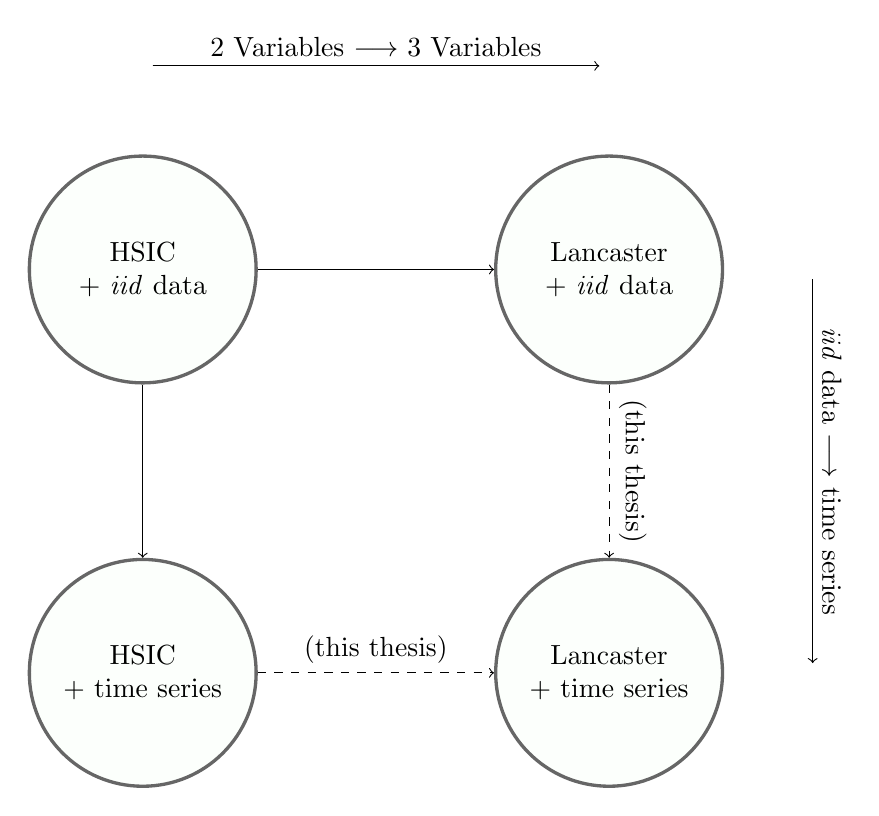
\begin{tikzpicture}[
roundnode/.style={circle, draw=black!60, fill=green!1, very thick, minimum size=10mm,text width=2.5cm,align=center},
]
%Nodes
\node[roundnode]      (bottomleft)                              {HSIC \\ + time series};
\node[roundnode]        (upleft)       [above=of bottomleft,yshift=1.2cm] {HSIC \\ + \emph{iid} data};
\node[roundnode]      (bottomright)       [right=of bottomleft,xshift=2cm] {Lancaster \\ + time series};
\node[roundnode]        (upright)       [right=of upleft,xshift=2cm] {Lancaster \\ + \emph{iid} data};
\node (A) [above=of upleft]{};
\node (B) [above=of upright]{};
%\node (C) [left=of upleft]{};
%\node (D) [left=of bottomleft]{}; 
\node (C) [right=of upright]{};
\node (D) [right=of bottomright]{}; 


%Lines
\draw[->] (upleft.south) -- (bottomleft.north);
\draw[dashed,->] (bottomleft.east) -- (bottomright.west) node [midway, above, sloped, dashed] (TextNode) {(this thesis)};;
\draw[dashed,->] (upright.south) -- (bottomright.north) node [midway, above, sloped, dashed] (TextNode) {(this thesis)};
\draw[->] (upleft.east) -- (upright.west);



\draw[->] (A) -- (B);
\draw (A) -- (B) node [midway, above, sloped] (TextNode) {2 Variables $\longrightarrow$ 3 Variables};

%\draw[<-] (D) -- (C);
%\draw (D) -- (C) node [midway, above, sloped] (TextNode) {timeseries $\longleftarrow$ \emph{iid}};
\draw[->] (C) -- (D);
\draw (C) -- (D) node [midway, above, sloped] (TextNode) {\emph{iid} data $\longrightarrow$ time series};
\end{tikzpicture}
\caption{A diagram to show how the work in this thesis relates to existing work. \label{thisthesis}}
\end{figure}



\newpage

\section{Background}
In this section, the background theory necessary to understand the result of this thesis is introduced. The author suggests that the reader mentally divide this theory into two categories: understanding the HSIC and Lancaster statistical tests in the case that our observations are drawn \emph{iid}; and understanding the conditions that must be met to be able to use the Wild Bootstrap to adapt these tests when our observations are not \emph{iid}. 

We will first give a very brief introduction to the theory of \emph{reproducing kernel Hilbert spaces (RKHSs)}. For further information, the interested reader may consult \cite{hofmann2008kernel}, \cite{scholkopf2002learning},\cite{berlinet2011reproducing}, \cite{steinwart2008support} and \cite{williams2006gaussian}. Our main objective here is to introduce the \emph{kernel mean embedding} \cite{smola2007hilbert}, a method that, subject to certain conditions, injectively embeds measures into a Hilbert space and so induces a metric on probability distributions. This method is the basis of our statistical tests.

Next the Hilbert-Schmidt Independence Criterion (HSIC), a statistical test for detecting dependence between two random variables, is introduced for the \emph{iid} case. Then, the Lancaster interaction, which can be viewed as a generalisation of HSIC to three random variables, is introduced, also for the \emph{iid} case. 

We then set the stage for describing how we may deal with non-\emph{iid} data. We will give a basic formal definition for certain types of time series. Then we will describe a common class of statistics known as V-statistics. Having done this, we will be able to describe the Wild Bootstrap.

%In \emph{Section 3}, we show that the conditions required to use the Wild Bootstrap on a test statistic are satisfied by the HSIC and Lancaster statistics.

\subsection{Kernel basics}
%\begin{itemize}
%\item NOTE: could follow layout of GreBouSmoSch05 to a certain extent
%\item also follow gretton12a, remember to cite this. (JMLR article)
%\item define a kernel (symmetric positive definite function).
%\item define gram matrix. note that symmetric positive definiteness of k implies K is always s.p.d.
%\item associated with a kernel is an rkhs
%\item can think of k(x,.) as being a function on curly X
%\item define kernel mean embedding
%\item say that you can approximate mean embedding empirically
%\item introduce mmd? at least mention it
%\item covariance operator! Define Hilbert Schmidt operators, say that they form a hilbert space. Can define kernel on $\mathcal{X}\times \mathcal{Y}$ via $\phi(X) \otimes \phi(Y)$ which lives in this Hilbert Schmidt space.
%\item explain computational rules that are needed, namely that $\langle u \otimes v , x \otimes y \rangle = \langle u, x \rangle \langle v, y \rangle$
%\item show how covariance operator and tensor product of averages relate to mean embeddings / empirical embeddings.
%\end{itemize}

\begin{definition}[Kernel] Let $\mathcal{X}$ be a non-empty set. A \emph{kernel on $\mathcal{X}$} is a function $k:\mathcal{X}\times \mathcal{X} \longrightarrow \mathbb{R}$ for which there exists a Hilbert space $\mathcal{H}$ and a \emph{feature map} $\phi: \mathcal{X} \longrightarrow \mathcal{H}$ such that, for all $x, y \in  \mathcal{H}$

\[k(x,y) = \langle \phi(x),\phi(y) \rangle_\mathcal{H}\]
\end{definition}

\begin{definition}[Gram matrix] Let $k$ be a kernel on $\mathcal{X}$ and suppose that $\mathcal{D} = \{X_1,\ldots,X_n \}$ is a set of samples from $\mathcal{X}$. The Gram matrix is an $n \times n$ matrix with entries

\[K_{ij} = k(X_i,X_j), \quad \quad i,j \in \{1,\ldots,n\}\]
\end{definition}

\begin{remark}[Notation]
Throughout this thesis, we will use the convention that lower case letters are used for kernels and the corresponding upper case letters are used for the corresponding Gram matrices.
\end{remark}

%\begin{remark}[Choices of definitions; thoughts on feature maps]
%There are alternative ways of defining kernels (for example, as a function for which the Gram matrix is always positive semi-definite). For the purposes of this thesis, it is easier to think of a kernel as satisfying the given definition, though the reader should note that in general it is possible to define kernels without knowing the associated feature map (or indeed there may be many possible feature maps that one could use for a single kernel). A reader that is new to kernel methods should bear in mind that although we know that a feature map exists, we may not wish to explicitly represent it. Indeed, part of the power of kernels is that they give us a window into an infinite dimensional feature space with only ever having to explicitly represent finite quantities.
%\end{remark}

\begin{definition}[Reproducing kernel Hilbert space]
Let $\mathcal{H}$ be a Hilbert space of $\mathbb{R}$-valued functions defined on a non-empty set $\mathcal{X}$. A function $k:\mathcal{X}\times \mathcal{X} \longrightarrow \mathbb{R}$ is a \emph{reproducing kernel} of $\mathcal{H}$, and $\mathcal{H}$ is a reproducing kernel Hilbert space (RKHS), if
\begin{enumerate}[(i)]
\item $\forall x \in \mathcal{X}$, $k(\cdot, x) \in \mathcal{H}$
\item $\forall x \in \mathcal{X}$, $\forall f \in \mathcal{H}$, $\langle f , k(\cdot, x) \rangle_\mathcal{H} = f(x)$
\end{enumerate}
\end{definition}

\begin{remark}[Feature maps]
There may be many possible choices of feature maps to represent any given kernel. We call $\phi(x) = k(\cdot,x)$ as written above the \emph{canonical feature map}. In general, it may not be useful (or even practically possible) to explicitly represent $\phi$. Indeed, part of the power of kernels is that we can implicitly work in a high (possibly infinite) dimensional feature space without ever having to explicitly represent it.
\end{remark}

The above definitions say that, given a reproducing kernel Hilbert space, we can take any point $x \in \mathcal{X}$ and embedd it in the RKHS as $\phi(x) = k(\cdot,x)$. This then allows us to evaluate any function $f \in \mathcal{H}$ at $x$ by taking an inner product: $f(x) = \langle f, \phi(x) \rangle_\mathcal{H}$.

Under certain conditions, we can extend this notion to embedding probability distributions. This allows us to calculate the \emph{expectation} of a function by taking its inner product with respect to the element in $\mathcal{H}$ corresponding to the embedding of the distribution. 

\begin{definition}[Mean embedding]
Let $\mathbb{P}_X$ be a probability measure on $\mathcal{X}$ and let $X \sim \mathbb{P}_X$ be a random variable on $\mathcal{X}$. The \emph{mean embedding} $\mu_{\mathbb{P}_X}$ of $\mathbb{P}_X$ is an element of $\mathcal{H}$ satisfying

\[\mathbb{E}_{X\sim \mathbb{P}_X} f(X) = \langle f, \mu_{\mathbb{P}_X} \rangle \]

for all $f \in \mathcal{H}$


\end{definition}

It is not obvious from this definition whether $\mu_{\mathbb{P}_X}$ exists. The following theorem provides a sufficient condition for this:

\begin{theorem}

Suppose that $k$ is measurable and that $\mathbb{E}_{X \sim \mathbb{P}_X} \sqrt{k(X,X)} < \infty$. Then $\mu_{\mathbb{P}_X} \in \mathcal{H}$.

Consequently, if $k$ is \emph{bounded} (ie $\exists C$ s.t.  $k(x,y) \leq C$ $\forall x,y \in \mathcal{X}$) then the mean embedding exists for any probability distribution on $\mathcal{X}$
\end{theorem}

For a proof of this, see \cite{sriperumbudur2010hilbert}. Throughout this thesis, we will assume that all kernels under consideration are bounded, and hence mean embeddings always exist.

\begin{remark}
For intuition, we can think of the mean embedding of a distribution as the expectation of an $\mathcal{H}$-valued random variable $\phi(X)$:

\[ \mu_{\mathbb{P}_X} = \mathbb{E}_{X\sim \mathbb{P}_X}[k(\cdot,X)] = \mathbb{E}_{X\sim \mathbb{P}_X}\phi(X)\]

\end{remark}



\begin{remark}[Distances between probability distributions]
Observe that the kernel mean embedding induces a map 

\begin{align*}
\{\text{Probability distributions on } \mathcal{X}\}&\longrightarrow \mathcal{H} \\
\mathbb{P} &\mapsto \mu_{\mathbb{P}}
\end{align*}

Provided this is injective, this induces a metric on $\{\text{Probability distributions on } \mathcal{X}\}$:

\begin{align*}
d(\mathbb{P},\mathbb{Q}) = \|\mu_{\mathbb{P}}-\mu_{\mathbb{Q}}\|
\end{align*}

Kernels for which this map is injective are known as \emph{characteristic}\cite{sriperumbudur2011universality}. It is not within the scope of this thesis to go into more detail, but it suffices to say that the Gaussian kernel (defined below) is characteristic.

\end{remark}

\begin{definition}[Gaussian kernel]
Suppose that $\mathcal{X} \subseteq \mathbb{R}^m$ for some $m \in \mathbb{N}$ The Gaussian kernel with bandwidth parameter $\sigma \in \mathbb{R}_{>0}$ is

\[ k_\sigma (x,y) = \exp (-\frac{\|x-y\|^2}{2\sigma^2}) \]

\end{definition}

\begin{theorem}
The Gaussian kernel is indeed a kernel which is moreover characteristic.
\end{theorem}

For proof, see Proposition 4.10 and Theorem 4.47 of \cite{steinwart2008support}.

\begin{remark}
Many kernel statistical tests, and in particular the ones that will be considered in this thesis, can be viewed as essentially exploiting this `metric on probability distributions'. For example, the MMD \cite{gretton2012kernel} is a test to see whether two samples have come from the same distribution. This uses the fact that $\| \mu_\mathbb{P} - \mu_\mathbb{Q} \|^2 = 0 \iff \mathbb{P} = \mathbb{Q}$, and then constructs a test working with finite samples based on this. We are interested here in independence testing - for example, does $\|\mu_{\mathbb{P}_{XY}} - \mu_{\mathbb{P}_{X}\mathbb{P}_{Y}}\|^2 = 0$? - and so we must build some more theory to be able to consider kernels on more than one random variable.
\end{remark}

We now follow closely \cite{gretton2005measuring}

\begin{definition}[Hilbert-Schmidt norm]
Suppose that $\mathcal{F}$ and $\mathcal{G}$ are separable Hilbert spaces with orthonormal bases $\{u_i\}$ and $\{v_i\}$ respectively, and suppose that $\mathcal{C}: \mathcal{G} \longrightarrow \mathcal{F}$ is a linear operator. Then, provided that the sum converges, the Hilbert-Schmidt (HS) norm of $\mathcal{C}$ is defined as

\[ \|\mathcal{C}\|_{HS}^2 : = \sum_{ij} \langle Cv_i, u_j \rangle_\mathcal{F}^2 \]

\end{definition}

\begin{definition}[Hilbert-Schmidt operators]
A linear operator $\mathcal{C}: \mathcal{G} \longrightarrow \mathcal{F}$ is called a Hilbert-Schmidt operator if its HS norm exists. The set of Hilbert-Schmidt operators from $\mathcal{G}$ to $\mathcal{F}$, denoted $HS(\mathcal{G},\mathcal{F})$, is a separable Hilbert space with inner product

\[ \langle C, D \rangle_{HS} := \sum_{ij} \langle Cv_i,u_j\rangle_\mathcal{F} \langle Dv_i,u_j\rangle_\mathcal{F} \]

\end{definition}

\begin{definition}[Tensor product]
Let $f \in  \mathcal{F}$ and $g \in  \mathcal{G}$. The tensor product operator $f\otimes g :  \mathcal{G} \longrightarrow  \mathcal{F}$ is defined as

\[ (f\otimes g) h := f\langle g,h \rangle_\mathcal{G} \quad \forall h \in  \mathcal{G}\]

\end{definition}

\begin{remark}
Note that for $f, a \in \mathcal{F}$ and $g, b \in \mathcal{G}$
\begin{align*}
\langle f\otimes g, a\otimes b \rangle_{HS} & =  \sum_{ij} \langle (f\otimes g)v_i ,u_j \rangle \langle  (a\otimes b)v_i ,u_j \rangle \\
& =  \sum_{ij} \langle \langle g,v_i \rangle f ,u_j \rangle \langle  \langle b,v_i \rangle a  ,u_j \rangle \\
&=   \sum_{ij}  \langle g,v_i \rangle \langle f ,u_j \rangle \langle b,v_i \rangle \langle   a  ,u_j \rangle \\
&=   \langle f ,a \rangle_{\mathcal{F}} \langle g,b \rangle_{\mathcal{G}}\\
\end{align*}

And in particular,

\begin{align*}
\|f\otimes g\|_{HS}^2 &= \langle f\otimes g, f\otimes g \rangle_{HS}\\
& = \langle f,f\rangle_\mathcal{F} \langle g, g \rangle_{\mathcal{G}}\\
\end{align*}

and so $f\otimes g \in HS(\mathcal{G},\mathcal{F})$ 

\end{remark}

\begin{remark}[Kernels on pairs of variables]
Suppose that $X$ and $Y$ are (not necessarily independent) random variables taking value in $\mathcal{X}$ and $\mathcal{Y}$ respectively. We consider the pair $(X,Y)$ to be a random variable taking value in $\mathcal{X} \times \mathcal{Y}$ with joint distribution $\mathbb{P}_{XY}$.

Suppose that $k$ is a kernel on $\mathcal{X}$ with canonical feature map $\phi$ and RKHS $\mathcal{F}$ and $l$ is a kernel on $\mathcal{Y}$ with canonical feature map $\psi$ and RKHS $\mathcal{G}$. We can construct from these a new kernel $z$ on $\mathcal{X} \times \mathcal{Y}$ via

\begin{align*}
z((x_1,y_1),(x_2,y_2)) &= \langle \phi(x_1)\otimes\psi(y_1) ,\phi(x_2)\otimes\psi(y_2)\rangle_{HS(\mathcal{G},\mathcal{F})}  \\
& = \langle \phi(x_1) ,\phi(x_2)\rangle_{\mathcal{F}} \langle \psi(y_1) ,\psi(y_2)\rangle_{\mathcal{G}}\\
& = k(x_1,x_2) l(y_1,y_2)
\end{align*}

Using this, we can embed the joint distribution $\mathbb{P}_{XY}$ via

\begin{align*}
\mu_{\mathbb{P}_{XY}}  &= \mathbb{E}_{(X,Y)\sim \mathbb{P}_{XY}}[ \phi(X)\otimes\psi(Y)]\\
&= \mathbb{E}_{XY}[ \phi(X)\otimes\psi(Y)]\\
\end{align*}

and the product of marginals

\begin{align*}
\mu_{\mathbb{P}_{X}\mathbb{P}_{Y}} &= \mathbb{E}_{(X,Y)\sim \mathbb{P}_{X}\mathbb{P}_{Y}}[ \phi(X)\otimes\psi(Y)] \\
&= \mathbb{E}_{X}\mathbb{E}_{Y}[ \phi(X)\otimes\psi(Y)]\\
&= \mathbb{E}_{X}[\phi(X)]\otimes\mathbb{E}_{Y}[ \psi(Y)]\\
&= \mu_{\mathbb{P}_{X}}\otimes \mu_{\mathbb{P}_{Y}} \\
\end{align*}

For shorthand, we write $\mu_{XY}$ instead of $\mu_{\mathbb{P}_{XY}}$, $\mu_{X}$ instead of $\mu_{\mathbb{P}_{X}}$, and $\mu_{Y}$ instead of $\mu_{\mathbb{P}_{Y}}$.

Throughout this thesis, we will assume that all kernels, including those defined over pairs and triples of variables, are characteristic.

\end{remark}


\subsection{Hilbert-Schmidt Independence Criterion (HSIC)}

We are now in a position to discuss HSIC. Again, this will only be a brief overview. For a more in depth explanation, see \cite{gretton2007kernel} and \cite{gretton2005measuring}. The problem we are interested in solving is the following:

\begin{problem}
Suppose we are given a set of \emph{iid} samples  $\{(X_i,Y_i), i=1,\ldots,n\}$ of random variables $X$ and $Y$ taking value in $\mathcal{X}$ and $\mathcal{Y}$ respectively. Can we tell if $X$ and $Y$ are independent? 

Equivalently, we may ask: does the joint distribution on $(X,Y)$ factorise into the product of marginals? ie, does $\mathbb{P}_{XY} = \mathbb{P}_{X}\mathbb{P}_{Y}$?
\end{problem}

Let us fix some notation. We assume that $k$ is a kernel on $\mathcal{X}$ with associated feature map $\phi$, and that $l$ is a kernel on $\mathcal{Y}$ with associated feature map $\psi$

In \cite{gretton2005measuring}, the \emph{cross-covariance operator is defined} to be

\begin{align*}
C_{XY} &:= \mathbb{E}_{XY}[(\phi(X) - \mu_X)\otimes(\psi(Y) - \mu_Y)]\\
&= \mathbb{E}_{XY}[\phi(X)\otimes\psi(Y)] - \mu_X\otimes \mu_Y\\
& = \mu_{XY} - \mu_X\otimes \mu_Y\\
\end{align*}

Observe that, since we assume the kernel on $(X,Y)$ to be characteristic, $C_{XY} = 0 \iff \mathbb{P}_{XY} = \mathbb{P}_X\mathbb{P}_Y$. We can exploit this to construct a statistical test for independence. We first define:

\begin{definition}[HSIC]

$HSIC[\mathbb{P}_{XY}] = \|C_{XY}\|_{HS}^2$
\end{definition}

Observe that $HSIC[\mathbb{P}_{XY}]$ can be written in terms of inner products of mean embeddings:

\begin{align*}
HSIC[\mathbb{P}_{XY}] &= \|C_{XY}\|_{HS}^2\\
&= \|\mu_{XY} - \mu_X\otimes \mu_Y\|^2 \\
& = \langle \mu_{XY} , \mu_{XY} \rangle - 2\langle \mu_{XY} , \mu_X\otimes \mu_Y\rangle + \langle\mu_X\otimes \mu_Y ,\mu_X\otimes \mu_Y \rangle \\
& = \langle \mathbb{E}_{XY}[\phi(X)\otimes\psi(Y)] , \mathbb{E}_{XY}[\phi(X)\otimes\psi(Y)] \rangle \\
& \quad \quad - 2\langle\mathbb{E}_{XY}[\phi(X)\otimes\psi(Y)] , \mathbb{E}_{X}[\phi(X)]\otimes\mathbb{E}_{Y}[\phi(Y)]\rangle  \\
& \quad \quad + \langle \mathbb{E}_{X}[\phi(X)]\otimes\mathbb{E}_{Y}[\phi(Y)] ,\mathbb{E}_{X}[\phi(X)]\otimes\mathbb{E}_{Y}[\phi(Y)] \rangle \\
%&=\mathbb{E}_{XY}\mathbb{E}_{X'Y'} k(X,X')l(Y,Y')\\
%& \quad \quad -2 \mathbb{E}_{XY}\mathbb{E}_{X'}\mathbb{E}_{Y'} k(X,X')l(Y,Y')\\
%& \quad \quad + \mathbb{E}_{X}\mathbb{E}_{Y}\mathbb{E}_{X'} \mathbb{E}_{Y'}k(X,X')l(Y,Y')
\end{align*}

In general we do not have access to $\mathbb{P}_{XY}$ and so we cannot evaluate $HSIC[\mathbb{P}_{XY}]$ (indeed, if we did we would not need to construct a complex statistical test to determine whether or not $\mathbb{P}_{XY}$ factorises!). Suppose that we are given independent samples $\mathcal{D} = \{(X_i,Y_i), i=1,\ldots,n\}$ drawn from $\mathbb{P}_{XY}$. We define the following quantities, which we can think of as estimating the mean embeddings as follows\footnote{This is a useful intuition for understanding HSIC, but to avoid having to consider technicalities we will not make this notion precise.}:

\begin{align*}
\tilde{\mu}_{XY}&: = \frac{1}{n} \sum_i \phi(X_i)\otimes\psi(Y_i)  \approx  \mathbb{E}_{XY}[\phi(X)\otimes\psi(Y)] = \mu_{XY}  \\
\tilde{\mu}_{X}&: = \frac{1}{n} \sum_i \phi(X_i)  \approx  \mathbb{E}_{X}\phi(X) = \mu_{X}  \\
\tilde{\mu}_{Y}&: = \frac{1}{n} \sum_i \phi(Y_i)  \approx  \mathbb{E}_{Y}\phi(Y) = \mu_{X}  \\
\end{align*}

This gives rise to a (biased) estimate which can be expressed in terms of the Gram matrices $K$ and $L$:

\begin{align*}
HSIC_b[\mathcal{D}] &= \|\tilde{\mu}_{XY} - \tilde{\mu}_X\otimes \tilde{\mu}_Y\|^2 \\
& = \langle \tilde{\mu}_{XY} , \tilde{\mu}_{XY} \rangle - 2\langle \tilde{\mu}_{XY} , \tilde{\mu}_X\otimes \tilde{\mu}_Y\rangle + \langle\tilde{\mu}_X\otimes \tilde{\mu}_Y ,\tilde{\mu}_X\otimes \tilde{\mu}_Y \rangle \\
& = \langle\frac{1}{n}\sum_i[\phi(X_i)\otimes\psi(Y_i)] ,\frac{1}{n}\sum_j[\phi(X_j)\otimes\psi(Y_j)] \rangle \\
& \quad \quad - 2\langle\frac{1}{n}\sum_i[\phi(X_i)\otimes\psi(Y_i)] , [\frac{1}{n}\sum_j\phi(X_j)]\otimes[\frac{1}{n}\sum_r\phi(Y_r)]\rangle  \\
& \quad \quad + \langle [\frac{1}{n}\sum_i\phi(X_i)]\otimes[\frac{1}{n}\sum_j\phi(Y_j)] ,[\frac{1}{n}\sum_r\phi(X_r)]\otimes[\frac{1}{n}\sum_s\phi(Y_s)] \rangle \\
&=\frac{1}{n^2}\sum_{ij}\langle\phi(X_i),\phi(X_j)\rangle\langle\psi(Y_i),\psi(Y_j)\rangle \\
& \quad \quad - \frac{2}{n^3}\sum_{ijr}\langle\phi(X_i),\phi(X_j)\rangle\langle\psi(Y_i),\psi(Y_r)\rangle \\
&\quad \quad+ \frac{1}{n^4}\sum_{ijrs}\langle\phi(X_i),\phi(X_r)\rangle\langle\psi(Y_j),\psi(Y_s)\rangle\\
&=\frac{1}{n^2}\sum_{ij}K_{ij}L_{ij} - \frac{2}{n^3}\sum_{ijr}K_{ij}L_{ir} + \frac{1}{n^4}\sum_{ijrs}K_{ir}L_{js}\\
\end{align*}

This empirical estimate of $HSIC$ converges to its population (ie true) value at a rate of $O(1/\sqrt{n})$ \cite{gretton2005kernel}\cite{gretton2005measuring}.

We wish to use this function of the observations as test statistic. The null hypothesis in our test, $\mathcal{H}_0$, is that $\mathbb{P}_{XY} = \mathbb{P}_{X}\mathbb{P}_{Y}$. The alternative hypothesis $\mathcal{H}_1$, is that $\mathbb{P}_{XY} \neq \mathbb{P}_{X}\mathbb{P}_{Y}$. Thus, under $\mathcal{H}_0$, $HSIC_b[\mathcal{D}] \longrightarrow 0$ and under $\mathcal{H}_1$, $HSIC_b[\mathcal{D}] \longrightarrow c$ for some $c > 0$ as the number of data grow.

$HSIC_b[\mathcal{D}]$ is a random variable and thus has some distribution. For any finite sample size we need to be able to estimate the distribution under the null hypothesis in order to be able to find a threshold value of the test statistic at which we would reject the null hypothesis. We do this using a \emph{permutation bootstrap} method to simulate draws of the statistic from its null distribution.

Observe that samples $(X_i,Y_i)$ are $iid$ for different $i$, and therefore $X_i$ will be independent of $Y_j$ for $i\neq j$ even if $X$ and $Y$ are dependent. By applying a permutation $\pi$ to the indices of one of the variables, we can therefore simulate a sample from the distribution $\mathbb{P}_{X}\mathbb{P}_{Y}$:

\[\mathcal{D}' = \{(X_i,Y_{\pi(i)}),\enspace i=1,\ldots,n \} \]

By simulating a large number of draws in this way, we can estimate the null distribution of the test statistic and calculate a threshold value, given a desired Type I error $\alpha$. 


In summary, the statistical test described above, HSIC, gives us a procedure for which rejection of the null implies that $\mathbb{P}_{XY}$ does not factorise. Since $HSIC_b[\mathcal{D}] \longrightarrow 0 \iff \mathcal{H}_0$ holds, the probability of falsely accepting the null hypothesis tends to zero for any fixed (non-factorising) distribution, and so HSIC is consistent.


\subsection{Lancaster statistic}

The Lancaster test is a natural generalisation of HSIC to three random variables, however as we will see it lacks consistency. We are interested in answering the following:

\begin{problem}
Suppose we are given a set of \emph{iid} samples $\{(X_i,Y_i,Z_i), i=1,\ldots,n\}$ of random variables $X$, $Y$ and $Z$ taking value in $\mathcal{X}$, $\mathcal{Y}$ and $\mathcal{Z}$ respectively. Can we tell if any of the variables are independent of the others? 

Equivalently, we may ask: does the joint distribution on $(X,Y,Z)$ factorise in some way? (For example, does $\mathbb{P}_{XYZ} = \mathbb{P}_{XY}\mathbb{P}_{Z}$?)
\end{problem}

In an ideal world, we would like to be able to construct a statistical test that returns a definitive \emph{yes} or \emph{no} to the above question, subject to diminishing Type I and II errors as the number of observations grows.

The Lancaster test does not quite do this. Instead, it is a test for which rejection of the null hypothesis implies that the joint distribution does not factorise. If the null hypothesis is not rejected, we cannot conclude whether the joint distribution factorises or not, as we will see shortly.

Before we describe the test, let us first fix some notation. We suppose that $X, Y$ and $Z$ are random variables taking value in $\mathcal{X}$, $\mathcal{Y}$ and $\mathcal{Z}$ respectively. We suppose that $k$, $l$ and $m$ are kernels on $\mathcal{X}$, $\mathcal{Y}$ and $\mathcal{Z}$ with canonical feature maps $\phi$, $\psi$ and $\omega$ respectively. We are given $iid$ samples $\mathcal{D} = \{(X_i,Y_i,Z_i), i=1,\ldots,n\}$. The Gram matrices with respect to these data are written $K$, $L$ and $M$. 

The Lancaster interaction measure is a signed measure, defined as follows:

\[\Delta_LP = \mathbb{P}_{XYZ} - \mathbb{P}_{XY}\mathbb{P}_{Z} - \mathbb{P}_{XZ}\mathbb{P}_{Y} - \mathbb{P}_{X}\mathbb{P}_{YZ} +2\mathbb{P}_{X}\mathbb{P}_{Y}\mathbb{P}_{Z} \]

\begin{claim} If any variable is independent of the other two, then the Lancaster interaction vanishes. That is, 

\[(X,Y) \independent Z \lor (X,Z) \independent Y \lor (Y,Z) \independent X \implies \Delta_LP = 0\]

\end{claim}

\begin{claimproof}
By symmetry, it suffices to consider the case $(X,Y) \independent Z$.

In this case, $\mathbb{P}_{XYZ} = \mathbb{P}_{XY}\mathbb{P}_{Z}$. By marginalising out $X$ or $Y$, we obtain  $\mathbb{P}_{YZ} = \mathbb{P}_{Y}\mathbb{P}_{Z}$ and  $\mathbb{P}_{XZ} = \mathbb{P}_{X}\mathbb{P}_{Z}$. Thus
\begin{align*}
\Delta_LP &= \mathbb{P}_{XYZ} - \mathbb{P}_{XY}\mathbb{P}_{Z} - \mathbb{P}_{XZ}\mathbb{P}_{Y} - \mathbb{P}_{X}\mathbb{P}_{YZ} +2\mathbb{P}_{X}\mathbb{P}_{Y}\mathbb{P}_{Z} \\
&= \mathbb{P}_{XY}\mathbb{P}_{Z} - \mathbb{P}_{XY}\mathbb{P}_{Z} - \mathbb{P}_{X}\mathbb{P}_{Y}\mathbb{P}_{Z} - \mathbb{P}_{X} \mathbb{P}_{Y}\mathbb{P}_{Z} +2\mathbb{P}_{X}\mathbb{P}_{Y}\mathbb{P}_{Z} \\
&= 0
\end{align*}
\end{claimproof}

Unfortunately, the reverse implication does not hold - see Table \ref{tab:lancaster_vanish} for an example of three binary variables with non-factorising joint distribution but vanishing Lancaster interaction\footnote{Note that this Table has been lifted directly from \cite{sejdinovic2013kernel}, and is not my own work.}.


\begin{table}
\caption{\label{tab:lancaster_vanish}{\footnotesize An example of three binary variables for which the joint distribution does not factorise, yet whose Lancaster interaction is zero. Note that this table is taken from \cite{sejdinovic2013kernel} as is not my own work.}}


\centering{}{\small }%
\begin{tabular}{|c||c|}
\hline 
{\small $P(0,0,0)=0.2$} & {\small $P(0,0,1)=0.1$}\tabularnewline
\hline 
{\small $P(0,1,0)=0.1$} & {\small $P(0,1,1)=0.1$}\tabularnewline
\hline 
\hline 
{\small $P(1,0,0)=0.1$} & {\small $P(1,0,1)=0.1$}\tabularnewline
\hline 
{\small $P(1,1,0)=0.1$} & {\small $P(1,1,1)=0.2$}\tabularnewline
\hline 
\end{tabular}
\end{table}


Generalising the tensor product notation introduced in the previous section, we can define the kernel $k\otimes l \otimes m$ on $\mathcal{X} \times \mathcal{Y} \times \mathcal{Z}$ with canonical feature map $\phi \otimes \psi \otimes \omega$ as:

\begin{align*}
k\otimes l \otimes m((x_1,y_1,z_1) ,(x_2,y_2,z_2) ) &=  \langle \phi(x_1)\otimes \psi(y_1) \otimes \omega(z_1) ,\phi(x_2)\otimes \psi(y_2) \otimes \omega(z_2) \rangle \\
& =  \langle \phi(x_1) , \phi(x_2) \rangle \langle \psi(y_1) , \psi(y_2) \rangle \langle \omega(z_1) , \omega(z_2) \rangle \\
&= k(x_1,x_2)l(y_1 ,y_2)m(z_1,z_2) 
\end{align*}

As such, we can define the mean embedding of the Lancaster interaction measure. For simplicity, we will refer to the embedded version of the signed measure also as $\Delta_LP$:

\begin{align*}
\Delta_LP &= \mu_{\mathbb{P}_{XYZ}} - \mu_{\mathbb{P}_{XY}\mathbb{P}_{Z}} - \mu_{\mathbb{P}_{XZ}\mathbb{P}_{Y}} - \mu_{\mathbb{P}_{X}\mathbb{P}_{YZ}} +2\mu_{\mathbb{P}_{X}\mathbb{P}_{Y}\mathbb{P}_{Z}} \\
&= \mathbb{E}_{(X,Y,Z) \sim \mathbb{P}_{XYZ}}\phi(X) \otimes \psi(Y) \otimes \omega(Z) -
\mathbb{E}_{(X,Y,Z) \sim \mathbb{P}_{XY}\mathbb{P}_{Z}}\phi(X) \otimes \psi(Y) \otimes \omega(Z) \\ &\quad -
\mathbb{E}_{(X,Y,Z) \sim \mathbb{P}_{XZ}\mathbb{P}_{Y}}\phi(X) \otimes \psi(Y) \otimes \omega(Z) -
\mathbb{E}_{(X,Y,Z) \sim \mathbb{P}_{X}\mathbb{P}_{YZ}}\phi(X) \otimes \psi(Y) \otimes \omega(Z) \\&\quad +
2\mathbb{E}_{(X,Y,Z) \sim \mathbb{P}_{X}\mathbb{P}_{Y}\mathbb{P}_{Z}}\phi(X) \otimes \psi(Y) \otimes \omega(Z) \\
&= \mathbb{E}_{XYZ}\phi(X) \otimes \psi(Y) \otimes \omega(Z) -
\mathbb{E}_{XY}\mathbb{E}_{Z}\phi(X) \otimes \psi(Y) \otimes \omega(Z) \\ &\quad -
\mathbb{E}_{XZ}\mathbb{E}_{Y}\phi(X) \otimes \psi(Y) \otimes \omega(Z) -
\mathbb{E}_{X}\mathbb{E}_{YZ}\phi(X) \otimes \psi(Y) \otimes \omega(Z) \\&\quad +
2\mathbb{E}_{X}\mathbb{E}_{Y}\mathbb{E}_{Z}\phi(X) \otimes \psi(Y) \otimes \omega(Z) 
\end{align*}

The squared norm $\| \Delta_LP \|_{\phi \otimes \psi \otimes \omega}^2$ is calculated by taking the inner product $\langle \Delta_LP,\Delta_LP \rangle$. This can therefore be expressed in terms of expectations of \[\langle \phi(X) , \phi(X') \rangle \langle \psi(Y) , \psi(Y') \rangle \langle \omega(Z) , \omega(Z') \rangle\] with respect to different factorisations of the joint.

Note that without knowing the distribution $\mathbb{P}_{XYZ}$, the we cannot calculate the squared norm. Given the observations $\mathcal{D}$, we can empirically estimate each of the $\mu_{\mathbb{P}}$ with an appropriate average over points in feature space. We can then use these empirical estimates to get an empirical estimate of the squared norm $\| \Delta_LP \|_{\phi \otimes \psi \otimes \omega}^2$. The empirical estimates we use are:

\begin{align*}
\hat\mu_{\mathbb{P}_{XYZ}} & =  \frac{1}{n}\sum_{i} \phi(X_i) \otimes \psi(Y_i) \otimes \omega(Z_i)\\
\hat\mu_{\mathbb{P}_{XY}\mathbb{P}_{Z}} & =  \frac{1}{n^2}\sum_{ij} \phi(X_i) \otimes \psi(Y_i) \otimes \omega(Z_j)\\
\hat\mu_{\mathbb{P}_{XZ}\mathbb{P}_{Y}} & = \frac{1}{n^2} \sum_{ij} \phi(X_i) \otimes \psi(Y_j) \otimes \omega(Z_i)\\
\hat\mu_{\mathbb{P}_{X}\mathbb{P}_{YZ}} & = \frac{1}{n^2} \sum_{ij} \phi(X_i) \otimes \psi(Y_j) \otimes \omega(Z_j)\\
\hat\mu_{\mathbb{P}_{X}\mathbb{P}_{Y}\mathbb{P}_{Z}} & =  \frac{1}{n^3}\sum_{ijk} \phi(X_i) \otimes \psi(Y_j) \otimes \omega(Z_k)\\
\end{align*}

Observe that the inner products between any two of these empirical mean embeddings can be expressed in terms of the Gram matrices. For example,

\begin{align*}
\langle \hat\mu_{\mathbb{P}_{XYZ}} ,\hat\mu_{\mathbb{P}_{XY}\mathbb{P}_{Z}}  \rangle &= \langle \frac{1}{n}\sum_{i} \phi(X_i) \otimes \psi(Y_i) \otimes \omega(Z_i) ,  \frac{1}{n^2}\sum_{jk} \phi(X_j) \otimes \psi(Y_j) \otimes \omega(Z_k)\rangle  \\
&= \frac{1}{n^3} \sum_{ijk}\langle  \phi(X_i) \otimes \psi(Y_i) \otimes \omega(Z_i) ,   \phi(X_j) \otimes \psi(Y_j) \otimes \omega(Z_k)\rangle  \\
&= \frac{1}{n^3} \sum_{ijk}\langle  \phi(X_i) , \phi(X_j)\rangle \langle \psi(Y_i), \psi(Y_j) \rangle \langle \omega(Z_i) , \omega(Z_k)\rangle  \\
& = \frac{1}{n^3} \sum_{ijk} K_{ij}L_{ij}M_{ik}  \\
\end{align*}

In this manner we can express  $\| \Delta_LP \|_{\phi \otimes \psi \otimes \omega}^2$ as a sum of 15 separate terms\footnote{There are $\binom{5}{2}=10$ combinations inner products of different terms, and 5 inner products of each term with itself.}, each written in terms of the Gram matrices. 






\begin{remark}
To summarise what we have done thus far: we have constructed a function of the observed data (a \emph{test statistic}) which estimates a quantity that, assuming that one of the variables $X$, $Y$ or $Z$ is independent of the other two, is zero.

Therefore, if our test statistic is `large' then we can conclude that none of the variables are independent of the others; that is to say that the joint distribution $\mathbb{P}_{XYZ}$ does not factorise.

To determine whether our test statistic is `large', we need to compare its value to the distribution of the statistic under the null distribution. As with HSIC, we use a \emph{permutation bootstrap} method to simulate samples under the null hypothesis.

Recall that the null hypothesis, $\mathcal{H}_0$, is that $\mathbb{P}_{XYZ}$ factorises in some way. Since there are three ways in which this can happen (namely $\mathbb{P}_{XYZ} = \mathbb{P}_{XY}\mathbb{P}_{Z}, \mathbb{P}_{XZ}\mathbb{P}_{Y}$ or  $\mathbb{P}_{X}\mathbb{P}_{YZ}$, noting that the case $\mathbb{P}_{XYZ} = \mathbb{P}_{X}\mathbb{P}_{Y}\mathbb{P}_{Z}$ is subsumed by each of these), we must test the three sub-hypotheses separately. If we reject all of the sub-hypotheses, then we reject the whole null hypothesis $\mathcal{H}_0$. Otherwise, we fail to reject the null. In this case, we cannot conclude anything about whether or not the joint factorises.
\end{remark}

To test each sub-hypothesis, we must estimate the corresponding null distribution. By symmetry, it suffices to explain how to estimate the distribution of the statistic under the assumption that $(X,Y)\independent Z$. Similarly to HSIC, we perform a permutation bootstrap procedure to generate simulated samples.  By applying a permutation $\pi$ to the indices of the $Z_i$, we generate a bootstrapped sample for which the dependence between $(X,Y)$ and $Z$ is broken:

\[ \mathcal{D}' = \{ (X_i, Y_i, Z_{\pi(i)}), \enspace i=1,\ldots, n\} \]

By generating many samples in this way, we can estimate any desired quantile for the threshold value of the statistic required to reject the null hypothesis.

As a footnote, observe finally that in the event that $\mathbb{P}_{XYZ} = \mathbb{P}_X\mathbb{P}_Y\mathbb{P}_Z$, the population Lancaster statistic will also be zero. Hence we can use this statistic to create a test for \emph{total independence}. We can simulate draws from the distribution of the statistic under the assumption of total independence by permuting the indices of two variables: for distinct permutations $\pi$ and $\sigma$, let

\[ \mathcal{D}' = \{ (X_i, Y_{\pi(i)}, Z_{\sigma(i)}), \enspace i=1,\ldots, n\} \]

We will not explore this further in this thesis.

\subsection{Resampling and the Wild Bootstrap}

%\begin{itemize}
%\item in both cases before we used a permutation method to estimate the null distribution
%\item this fails in the non-iid case. give examples to illustrate this
%\item instead, we need a more sophisticated method to estimate the null distribution
%\item the wild bootstrap comes to our rescue. However, it can only be used in certain circumstances
%\item these fall into two categories: conditions on the observations, and conditions on the test statistic.
%\item introduce timeseries stuff, and talk about $\tau$-dependence
%\item introduce V-statistics, say that many statistics can be viewed as v-statistics and that under the null hypothesis these are often degenerate.
%\item maybe talk about the fact that we normalise the test statistic because under the null the normalised test statistic converges to a random variable, (but under the alternative hypothesis, if the \emph{un}-normalised test statistic would have converged to a non-zero constant, the normalised test statistic diverges)
%\item wild bootstrap:  this gives a method to sample from the null under certain conditions that do allow for timeseries.
%\item state the assumptions of the hypothesis
%\end{itemize}

In the descriptions of the procedures for both the HSIC and Lancaster statistical tests above, recall that in order to simulate samples of the test statistic under the null distribution, we permuted the indices of one of the variables. In the case that our observations are not \emph{iid} but are rather drawn from a process with some temporal dependence, this procedure will fail to simulate samples from the correct distribution. Indeed, suppose we take a draw from such a process $(X_i)_{i=1}^n$ and scramble the indices to get a new, simulated draw $(X_{\pi(i)})_{i=1}^n$. The temporal dependence between consecutive $X_i$s will be broken and so the simulated draw will not have the same statistical properties as the true sample.

It follows that we were to try using the permutation methods with non-\emph{iid} data, we may incorrectly set the threshold value of the test statistic required to reject the null hypothesis for any given specificity since we would in fact not be simulating samples from the null distribution of the test statistic\footnote{This is explored further in Example 4 in the Experiments section}.

Instead, we need a more sophisticated bootstrap resampling method. The Wild Bootstrap \cite{leucht2013dependent} is a scheme that can be used to simulate samples under the null distribution, provided that certain conditions are satisfied. These conditions fall into two categories: first, conditions on the underlying process from which the observations are drawn; second, conditions on the test statistic itself.

Before discussing the Wild Bootstrap itself, it is first necessary to provide background information to understand these conditions. In the following subsections, we will first introduce some formal concepts relating to time series, then the concept of a V-statistic, after which we will be well-equipped to discuss the Wild Bootstrap.




\subsubsection{Timeseries}
%\begin{itemize}
%\item say we are using timeseries, not iid data. This messes up the permuation approach. Before progressing further we need to give some background.
%\item Give formal definitions of two types of `memories' that a process can have
%\item $\beta$-mixing
%\item $\tau$-mixing
%\item prove that if $(X_t,Y_t,Z_t)$ is $\beta$- mixing, then so are $(X_t,Y_t)$ and $(Z_t)$. We need this for the central limit theorem later on.
%\end{itemize}

In this thesis we are concerned with extending the HSIC and Lancaster tests to situations in which the \emph{iid} assumption on the observations does not hold. We consider time series, ie data drawn from a random process in which successive observations are dependent on previous observations. There are various formalisations of this `memory' or mixing. Here we consider the two which are relevant to this thesis. For more information about mixing, see \cite{doukhan1994mixing}\cite{bradley2005basic}\cite{dedecker2007weak}.

\begin{definition}
A process $(X_t)_{t}$ is \emph{$\tau$-mixing} if $\tau(r) \longrightarrow 0$ as $r\longrightarrow \infty$, where

\[\tau(r) = \sup_{l\in \mathbb{N}} \frac{1}{l} \sup_{r\leq i_1 \leq \ldots \leq i_l} \tau(\mathcal{F}_0,(X_{i_1}, \ldots, X_{i_l})) \longrightarrow 0\]

where

\[ \tau(\mathcal{M},X) = \mathbb{E} (\sup_{g \in \Lambda} | \int g(t) \mathbb{P}_{X|\mathcal{M}}(dt) -  \int g(t) \mathbb{P}_{X}(dt) |)\]

\end{definition}

\begin{definition}
A process $(X_t)_{t}$ is \emph{$\beta$-mixing} (also known as \emph{absolutely regular}) if $\beta(m) \longrightarrow 0$ as $m\longrightarrow \infty$, where

\[ \beta(m) = \frac{1}{2} \sup_n \sup \sum_{i=1}^I \sum_{j=1}^J | \mathbb{P}(A_i \cap B_j) - \mathbb{P}(A_i)\mathbb{P}(B_j)| \]

where the second supremum is taken  over all finite partitions $\{A_1,\ldots, A_I \}$ and  $\{B_1,\ldots, B_J\}$ of the sample space such that $A_i \in \mathcal{A}_1^n$ and $B_j \in \mathcal{A}_{n+m}^\infty$ and $\mathcal{A}_b^c = \sigma(X_b,X_{b+1},\ldots,X_{c})$
\end{definition}

The concept of $\beta$-mixing will be invoked when applying a central limit theorem in the next section. We will also need the following lemma:

\begin{lemma}\label{lemma:beta}
Suppose that the process $(X_t,Y_t,Z_t)_t$ is $\beta$-mixing. Then any `sub-process' is also $\beta$-mixing (for example $(X_t,Y_t)_t$ or $(X_t)_t$)
\end{lemma}

\begin{claimproof} Let us consider $(X_t,Y_t)_t$.
Let us call $\beta_{XYZ}(m)$ the coefficients for the process $(X_t,Y_t,Z_t)_t$, and $\beta_{XY}(m)$ the coefficients for the process $(X_t,Y_t)_t$. 

Observe that for $A \in \sigma((X_b,Y_b),\ldots, (X_c,Y_c))$, it is the case that $A \times \mathcal{Z} \in \sigma((X_b,Y_b,Z_b),\ldots, (X_c,Y_c,Z_c))$ and $\mathbb{P}_{XY}(A) = \mathbb{P}_{XYZ}(A\times \mathcal{Z})$.

Thus

\begin{align*}
\beta_{XY}(m) &= \frac{1}{2} \sup_n \sup_{ \{A_i^{XY} \}, \{B_j^{XY} \} } \sum_{i=1}^I \sum_{j=1}^J | \mathbb{P}_{XY}(A_i^{XY} \cap B_j^{XY}) - \mathbb{P}_{XYZ}(A_i^{XY})\mathbb{P}_{XYZ}(B_j^{XY})| \\
&= \frac{1}{2} \sup_n \sup_{ \{A_i^{XY} \}, \{B_j^{XY} \} } \sum_{i=1}^I \sum_{j=1}^J | \mathbb{P}_{XYZ}((A_i^{XY}\times \mathcal{Z}) \cap (B_j^{XY} \times \mathcal{Z})) \\& \quad \quad\quad \quad \quad \quad\quad \quad \quad \quad\quad \quad- \mathbb{P}_{XYZ}(A_i^{XY}\times \mathcal{Z})\mathbb{P}_{XYZ}(B_j^{XY} \times \mathcal{Z})| \\
& \leq \frac{1}{2} \sup_n \sup_{ \{A_i^{XYZ} \}, \{B_j^{XYZ} \} } \sum_{i=1}^I \sum_{j=1}^J | \mathbb{P}_{XYZ}(A_i^{XYZ} \cap B_j^{XYZ}) - \mathbb{P}_{XYZ}(A_i^{XYZ})\mathbb{P}_{XYZ}(B_j^{XYZ})| \\
& = \beta_{XYZ}(m)
\end{align*}

Thus we have shown that  $\beta_{XYZ}(m) \longrightarrow 0 \implies \beta_{XY}(m) \longrightarrow 0$. That is, if  $(X_t,Y_t,Z_t)_t$ is $\beta$-mixing then so is  $(X_t,Y_t)_t$ 

A similar argument holds for any other sub-process.
\end{claimproof}


\subsubsection{V-statistics (and U-statistics)}

For an in-depth introduction to V- and U-statistics, see \cite{serfling2009approximation}.

Suppose that $X_1,X_2,\ldots$ are drawn $iid$ from a distribution $\mathbb{P}$, and that $\theta =  \theta (\mathbb{P})$ is a function of the distribution for which there is an unbiased estimator, where $h$ is a symmetric function of the observations \cite{serfling2009approximation}:

\[ \theta(\mathbb{P}) = \mathbb{E}_{X_i \sim \mathbb{P}}[h(X_1,\ldots,X_m)]\]

We call $h$ a \emph{core}, and we call its number of arguments its \emph{degree}. Given observations $\mathcal{S}_n = \{X_1,X_2,\ldots,X_n\}$ with $n\geq m$, the corresponding U-statistic is denoted

\[U =  U(h, \mathcal{S}_n) = \frac{1}{\binom{n}{m}}\sum_c h(X_{i_1},X_{i_2},\ldots,X_{i_m}) \]

where $c$ runs over each of the $\binom{n}{m}$ choices of $m$ distinct elements $\{i_1,i_2,\ldots,i_m\}$ from $\{1,2,\ldots,n\}$

V-statistics are closely related. Instead of summing over distinct observations $X_i$, we sum over all combinations of the observations of size $m$ with replacement. That is,

\[V = V(h,\mathcal{S}_n) = \frac{1}{n^m} \sum_{i_1 = 1}^{n} \sum_{i_2 = 1}^{n} \ldots \sum_{i_m = 1}^{n} h(X_{i_1}, X_{i_2},\ldots,X_{i_m})\]


$U$ is an unbiased estimator, and moreover it is the \emph{minimum variance unbiased estimator} for $\theta$ given the observations $\mathcal{S}_n$ \cite{serfling2009approximation}.

V-statistics are not unbiased, though they asymptotically approach their U-statistic counterparts, with convergence that is dependent on properties of the core $h$. 

In particular, we draw attention to the fact that both $U(h,\mathcal{S}_n)$ and $V(h,\mathcal{S}_n)$ converge to the expectation of the core $h$ as $n\longrightarrow \infty$.

We say that $nV(h,\mathcal{S}_n)$ is a \emph{normalised} V-statistic. In this thesis we will restrict ourselves to considering V-statistics of degree two, that is $h = h(X_1,X_2)$. We say that such a core is \emph{degenerate} if, for any $x_1$ and for $X_2 \sim \mathbb{P}$, $\mathbb{E}_{X_2}[h(x_1,X_2)] = 0$. If a V-statistic has a degenerate core, we say that it is a \emph{degenerate V-statistic}.



Note that if $V(h,\mathcal{S}_n)$ is degenerate, then $V \longrightarrow \mathbb{E}_{X_1,X_2}[h(X_1,X_2)] = 0$ as $n \longrightarrow \infty$. It can be shown that a normalised V-statistic with a degenerate core converges to a random variable \cite{serfling2009approximation}.

Observe that if $\mathbb{E}_{X_1,X_2}[h(X_1,X_2)] \neq 0$, then $nV(h,\mathcal{S}_n) \longrightarrow \infty$ as $n\longrightarrow \infty$.

Relevant to the above two statements is the fact that many kernel test statistics can be viewed as normalised V-statistics which, under the null hypothesis, are degenerate. If under the alternative hypothesis the test statistic diverges, then the test is consistent.

The main result of this thesis is to show that, under the null hypothesis, they are asymptotically equal to degenerate V-statistics.


%HSIC:
%
%\begin{align*}
%HSIC_b &= \frac{1}{n^2}(\tilde{K}\circ \tilde{L})_{++} \\
%& = \frac{1}{n^2} \sum_{ij} \tilde{k}(X_i,X_j)\tilde{l}(Y_i,Y_j) \\
%& = \frac{1}{n^2} \sum_{ij} h(S_i,S_j)\\
%& = V(h,\mathcal{S})
%\end{align*}
%
%where $S_i = (X_i,Y_i)$ and we define $h(S_i,S_j) = \tilde{k}(X_i,X_j)\tilde{l}(Y_i,Y_j)$. 
%
%
%Lancaster:
%
%\begin{align*}
%\|\Delta_LP\|^2 &= \frac{1}{n^2}(\tilde{K}\circ \tilde{L}\circ \tilde{M})_{++} \\
%& = \frac{1}{n^2} \sum_{ij} \tilde{k}(X_i,X_j)\tilde{l}(Y_i,Y_j)\tilde{m}(Z_i,Z_j) \\
%& = \frac{1}{n^2} \sum_{ij} h(S_i,S_j)\\
%& = V(h,\mathcal{S})
%\end{align*}
%
%where $S_i = (X_i,Y_i,Z_i)$ and we define $h(S_i,S_j) = \tilde{k}(X_i,X_j)\tilde{l}(Y_i,Y_j)\tilde{m}(Z_i,Z_j)$. 

\subsubsection{The Wild Bootstrap}

We are now equipped to discuss the Wild Bootstrap. Recall that the problem we face with using time series for HSIC and Lancaster is that the permutation methods to resample from the null distribution of the test statistics fails. The Wild Bootstrap provides a method to sample from the correct null distribution.

Suppose we have a test statistic that is a normalised V-statistic $nV$ with core $h$ of degree two, and suppose further that \cite{leucht2013dependent}\cite{chwialkowski2014wild}:

\begin{enumerate}[(1)]
\item \emph{Conditions on the observations:} Our observations $\mathcal{D}_n = (S_t)_{t=1}^n$ are drawn from a strictly stationary, $\tau$-dependent process with $\sum_{r=1}^\infty r^2 \sqrt{\tau(r)} < \infty$

\item \emph{Conditions on the test statistic}:
\begin{enumerate}[(i)]
\item $h$ is a bounded kernel on $\mathcal{S}$, where each $S_i$ takes value in $\mathcal{S}$
\item $h$ is degenerate as a core.
\item $h$ is Lipschitz continuous.
\end{enumerate}
\end{enumerate}

Our normalised V-statistic can be written

\[nV(h,\mathcal{D}_n) = \frac{1}{n} \sum_{ij} h(S_i,S_j)\]

We define the following two bootstrapped statistics \cite{chwialkowski2014wild}:

\begin{align*}
nV_{b1}(h,\mathcal{D}_n)& := \frac{1}{n} \sum_{ij} W_{i,n}W_{j,n}h(S_i,S_j) \\
nV_{b2}(h,\mathcal{D}_n)& := \frac{1}{n} \sum_{ij} \tilde{W}_{i,n}\tilde{W}_{j,n}h(S_i,S_j) \\
\end{align*}

where $(W_{t,n})_{1\leq t \leq n}$ is known as the \emph{auxiliary wild bootstrap process} and $\tilde{W}_{t,n} = W_{t,n} - \frac{1}{n} \sum_i W_{i,n}$. We suppose that this process satisfies the following assumption \cite{chwialkowski2014wild}: 

\begin{enumerate}[(1)]
  \setcounter{enumi}{2}
  \item \emph{Conditions on bootstrap process}: $(W_{t,n})_{1\leq t \leq n}$ is a row-wise strictly stationary triangular aray independent of all $S_t$ such that $\mathbb{E}W_{t,n} = 0$ and $\sup_n \mathbb{E}|W_{t,n}^{2+\sigma}| < \infty$ for some $\sigma > 0$. The autocovariance of the process is given by $cov(W_{s,n},W_{t,n}) = \rho(|s-t|/l_n)$ for some function $\rho$, such that $\lim_{u \longrightarrow 0} \rho (u) = 1$ and $\sum_{r=1}^{n-1} \rho(|r|/l_n) = O(l_n)$. The sequence $(l_n)$ is taken such that $l_n = o(n)$ and $lim_{n\longrightarrow \infty} l_n = \infty$. The variables $W_{t,n}$ are $\tau$-weakly dependent with coefficients $\tau (r) \leq C\zeta^{ \frac{r}{l_n}}$ for $r = 1,...,n$, $\zeta \in (0,1)$ and $C <\infty$
\end{enumerate}



A simple example of a process satisfying these properties is given by \cite{chwialkowski2014wild}\cite{leucht2013dependent}:

\[ W_{t,n} = e^{-1/l_n} W_{t-1,n} + \sqrt{1 - e^{-2/l_n} \epsilon_t} \]

where $W_{0,n}$ and $\epsilon_1,\ldots,\epsilon_n$ are independent standard normal random variables. 


\cite{leucht2013dependent} demonstrates the following result.

\begin{theorem} [Leucht]
Assume that conditions \emph{(1)}, \emph{(2)} and \emph{(3)} above hold. Then $nV, nV_{b1}$ and $nV_{b2}$ converge to the same distribution. In particular,

\[nV, \enskip nV_{b1}, \enskip nV_{b2}  \overset{d}{\longrightarrow} Z :=  \sum_k \lambda_k Z_k^2 \]

where $(Z_k)_k$ is a sequence of centred, jointly normal random variables with $cov(Z_j,Z_k) = \sum_{r=-\infty}^{\infty} cov(\Phi_j(X_0),\Phi_k(X_r))$, and $(\lambda_k)_k$ and $(\Phi_k)_k$ are the sequences of non-zero eigenvalues and the corresponding eigenfunctions of $\mathbb{E}[h(x,X_0)\Phi(X_0)] = \lambda \Phi(x)$
\end{theorem}

The particular distribution to which the test statistic and the bootstrapped statistics converge is not particularly important. The important thing about this theorem is that firstly, the test statistic does converge to some random variable, and that secondly we can simulate samples from this distribution using the bootstrapped statistics. Thus, provided that our observations satisfy (1) and that under the null hypothesis our test statistic satisfies (2), we now have a method to estimate the null distribution of our test statistic. 

In this thesis we are primarily concerned with condition (2) above: the aim is essentially to show that the test statistics for HSIC and Lancaster satisfy this. However, before we continue it is worth briefly considering conditions (1) and (3) as they suggest further directions for research. 

When can we say with confidence that observations have indeed been drawn from a process satisfying (1)?

As stated in the explanation of (3), it is relatively simple to write down a process that satisfies (3). However, there will exist many other processes that one could consider - indeed, even in the one written down, the choice of $l_n$ is open. As mentioned in \cite{leucht2013dependent}, in a similar method by Shao \cite{shao2010dependent}, the parameter choice of $l_n$ was not found to be very important. Further investigation into this or of other choices of bootstrap processes would be interesting, though in a different direction to the nature of the work done in this thesis.

\subsection{Summary}
\begin{itemize}
\item HSIC is a statistical test for detecting dependence between two random variables.
\item Lancaster is a statistical test for detecting dependence between three random variables. If we reject the null hypothesis, we conclude that there is no factorisation of the joint; if we do not reject the null hypothesis, we cannot conclude anything.
\item When the observed data are drawn \emph{iid}, it is possible to resample from the null distributions for both HSIC and Lancaster using permutation resampling. When the observed data are \emph{not iid}, this method is not valid.
\item The Wild Bootstrap is a method that enables simulated samples of a test statistic to be drawn under certain conditions. These are:
\begin{enumerate}[(i)]
	\item The observed data must be drawn from a $\tau$-mixing process
	\item The test statistic must be a V-statistic with a core that is a degenerate, Lipschitz continuous kernel	
\end{enumerate}
\end{itemize}

The objective of the following section is to show that, under their null hypotheses, Lancaster and HSIC satisfy condition (ii) above.

\newpage

\section{Main theoretical result}
In this section, a result is proved that implies the Wild Bootstrap can be applied to the Lancaster test statistic. This is the major new theoretical contribution of this work. Furthermore, this proof can be adapted to give a simpler proof that the Wild Bootstrap can be applied to HSIC. This is not new knowledge, however the previous proof given in \cite{chwialkowski2014kernel} was longer and relied on more advanced theory of U- and V- statistics, including the Hoeffding decomposition \cite{serfling2009approximation}. The reader should note that although the new proof given here is shorter, some of the complexity of the argument is simply deferred to the proof of a Hilbert space Central Limit Theorem for time series \cite{dehling2015bootstrap}.

The result which will be proved is that, under their respective null hypotheses, the normalised HSIC and Lancaster statistics are asymptotically V-statistics with cores that are degenerate kernels. 

The layout of this section is as follows. First, notation will be set up. Second, the result will be proved for HSIC. Third, the result will be proved for Lancaster. The proof ideas are essentially the same for the two statistics; the main difference is that the proof for Lancaster involves considering the asymptotic properties of many more terms than HSIC and is for this reason significantly longer, though not particularly more conceptually involved.

\subsection{Notation}

Let $k$ be a kernel with canonical feature map $\phi$. Given observations $X_i, \quad i=1,2,\ldots n$ let $K$ be the gram matrix such that $K_{ij} = k(X_i,X_j) =  \langle \phi(X_i),\phi(X_j) \rangle$.

Let $\tilde{\mu}_X = \frac{1}{n}\sum_{i=1}^{n} \phi(X_i)$ and let $\tilde{K}_{ij} = \langle \phi(X_i) - \tilde{\mu}_X, \phi(X_j) - \tilde{\mu}_X \rangle$. We call $\tilde{K}$ an \emph{empirically} centred gram matrix.

Let $\mu_X = \mathbb{E}_X\phi(X)$ and let $\bar{K}_{ij} = \langle \phi(X_i) - \mu_X, \phi(X_j) - \mu_X \rangle$. We call $\bar{K}$ an \emph{population} centred gram matrix.

Note that we cannot in general explicitly represent the feature mapped observations, and even when we can it may not be desirable to do so. We are, however, able to write the empirically centred gram matrix $\tilde{K}$ just in terms of values of the original matrix $K$, and the population centred gram matrix $\bar{K}$ in terms of $K$ and expectations of the kernel $k$. Indeed, by simply expanding the sum:

\begin{align*}
\tilde{K}_{ij}  & = \langle \phi(X_i) - \tilde{\mu}_X, \phi(X_j) - \tilde{\mu}_X \rangle \\
& =  \langle \phi(X_i) - \frac{1}{n} \sum_k\phi(X_k), \phi(X_j) - \frac{1}{n} \sum_l \phi(X_l) \rangle \\
& =  \langle \phi(X_i), \phi(X_j) \rangle  - \frac{1}{n} \sum_k \langle \phi(X_k), \phi(X_j) \rangle - \frac{1}{n} \sum_l \langle \phi(X_i) ,  \phi(X_l) \rangle + \frac{1}{n^2}  \sum_k \sum_l \langle \phi(X_k),  \phi(X_l) \rangle \\
& = K_{ij} - \frac{1}{n} \sum_k K_{kj} -\frac{1}{n}  \sum_l K_{il} + \frac{1}{n^2} \sum_{kl} K_{kl} \\
\end{align*}

For notational ease, we here introduce the following notational convention. For any matrix $A$, define

\begin{align*}
A_{i+} & = \sum_j A_{ij} \\
A_{+j} & = \sum_i A_{ij} \\
A_{++} & = \sum_{ij} A_{ij} \\
\end{align*}
If additionally $A$ is symmetric, we write
\begin{align*}
(A_+)_{ij} = A_{+j} = A_{j+}
\end{align*}
Hence we can write

\begin{align*}
\tilde{K}_{ij}  & = K_{ij} -\frac{1}{n}  K_{+j} - \frac{1}{n}  K_{i+} + \frac{1}{n^2} K_{++}
\end{align*}

Observe that this gives a method to convert an empirically-uncentred gram matrix into a centred one. For each entry, subtract the corresponding row and column averages and add the whole matrix average.

\begin{remark}The average value of any row or column of an empirically centred gram matrix is zero
\end{remark}


We can expand the population centred $\bar{K}$ in a similar fashion, expressing it in terms of expectations of the original kernel function $k$. In the following, $X$ and $X'$ are independent copies of the original random variable.

\begin{align*}
\bar{K}_{ij}  & = \langle \phi(X_i) - \mu_X, \phi(X_j) - \mu_X \rangle \\
  & = \langle \phi(X_i) - \mathbb{E}_X\phi(X), \phi(X_j) -\mathbb{E}_{X'}\phi(X') \rangle \\
  & = \langle \phi(X_i), \phi(X_j) \rangle  -  \mathbb{E}_X \langle \phi(X), \phi(X_j) \rangle -  \mathbb{E}_{X'} \langle \phi(X_i) , \phi(X') \rangle +   \mathbb{E}_X \mathbb{E}_{X'} \langle \phi(X), \phi(X') \rangle \\
& = k(X_i,X_j)  -  \mathbb{E}_X k(X,X_j) -  \mathbb{E}_{X'} k(X_i,X') +   \mathbb{E}_X \mathbb{E}_{X'} k(X,X') \\
\end{align*}

Similarly, we define the population centred kernel $\bar{k}$ similar to the above.

\begin{align*}
\bar{k}(X_i,X_j) = k(X_i,X_j)  -  \mathbb{E}_X k(X,X_j) -  \mathbb{E}_{X'} k(X_i,X') +   \mathbb{E}_X \mathbb{E}_{X'} k(X,X') \\
\end{align*}

We define the \emph{population centred} feature map $\bar{\phi}(X) := \phi(X) - \mu_X$. Note that since $\bar{k}$ corresponds to an inner product between points mapped under the feature map $\bar{\phi}$, $\bar{k}$ is indeed a valid kernel.

\begin{remark}
$\bar{k}$ is a degenerate kernel. Indeed, observe also that for any $x$,

\begin{align*}
\mathbb{E}_{X^*}\bar{k}(x,X^*) & =  \mathbb{E}_{X^*}k(x,X^*)  -  \mathbb{E}_X \mathbb{E}_{X^*} k(X,X^*) -  \mathbb{E}_{X'} k(x,X') +   \mathbb{E}_X \mathbb{E}_{X'} k(X,X') \\
& = 0\\
\end{align*}
\end{remark}

We denote by $\circ$ the Hadamard product, such that for any two matrices $K$ and $L$ of equal dimension, $(K\circ L)_{ij} = K_{ij}L_{ij}$.

Finally, throughout this thesis we will use at most 3 random variables and their associated feature maps and gram matrices. The random variables will always be referred to as $X, Y$ and $Z$. The associated kernels are denoted $k, l$ and $m$ respectively. The associated gram matrices are denoted $K, L$ and $M$ respectively. The associated feature maps are denoted $\phi, \psi$ and $\omega$ respectively.


\subsection{HSIC}

Recall that given samples $X_i, Y_i,  i=1,\ldots,n$, kernels $k$ on $\mathcal{X}$ and $l$ on $\mathcal{Y}$ and associated gram matrices $K$ and $L$, the biased statistic for HSIC is defined by

\begin{align*}
HSIC_b &= \frac{1}{n^2}\sum_{ij}K_{ij}L_{ij} - \frac{2}{n^3}\sum_{ijr}K_{ij}L_{jr} + \frac{1}{n^4}\sum_{ijrs}K_{ij}L_{rs}\\
& = \frac{1}{n^2}(K\circ L)_{++} - \frac{2}{n^3}(KL)_{++} + \frac{1}{n^4}K_{++}L_{++}\\
\end{align*}
In this section it will be shown that under the null hypothesis that $X$ and $Y$ are independent, the normalised statistic for HSIC is asymptotically a degenerate V-statistic. This degenerate V-statistic can then have the Wild Bootstrap applied to it to resample under the null hypothesis. We will first show that
\begin{align*}
nHSIC_b = \frac{1}{n}(\bar{K}\circ \bar{L})_{++} - \frac{2}{n^2}(\bar{K}\bar{L})_{++} + \frac{1}{n^3}\bar{K}_{++}\bar{L}_{++} \tag{$\dagger$}\\
\end{align*}

then show that the latter two terms in the above equation tend to 0 as $n \longrightarrow \infty$. Finally we will show that $\frac{1}{n}(\bar{K}\circ \bar{L})_{++}$ is a normalised degenerate V-statistic.

\begin{claim}\label{claim:HSICinvariant}

Let $\alpha$ and $\beta$ be fixed elements of the Hilbert Spaces in which $\phi(X)$ and $\psi(Y)$ take value respectively. Define $\phi'(X) = \phi(X) - \alpha$ and $\psi'(Y) = \psi(Y) - \beta$.

\[\frac{1}{n^2}(\tilde{K}\circ\tilde{L})_{++} = \frac{1}{n^2}(K'\circ L')_{++} - \frac{2}{n^3}(K'L')_{++} + \frac{1}{n^4}K'_{++}L'_{++}\]

where $K'_{ij} = \langle \phi'(X_i), \phi'(X_j) \rangle$ and $L'_{ij} = \langle \psi'(Y_i), \psi'(Y_j) \rangle$. 


In particular, taking $\alpha = \mu_X$ and $\beta  = \mu_Y$, observe that

\begin{align*}
\frac{1}{n^2} (\tilde{K}\circ \tilde{L})_{++} = \frac{1}{n^2}(\bar{K}\circ \bar{L})_{++} - \frac{2}{n^3}(\bar{K}\bar{L})_{++} + \frac{1}{n^4}\bar{K}_{++}\bar{L}_{++}
\end{align*}

And taking $\alpha = 0$ and $\beta = 0$,

\begin{align*}
\frac{1}{n^2} (\tilde{K}\circ \tilde{L})_{++} = HSIC_b
\end{align*}

and hence $(\dagger)$ is true.

\end{claim}
\begin{claimproof}
Given feature maps $\phi$ and $\psi$ and observations $\mathcal{D} = \{X_i, Y_i, i=1,\ldots,n\}$ define 

\begin{align*}
T(\phi, \psi, \mathcal{D}) = \frac{1}{n^2} \mathlarger{\mathlarger{\sum_{ij}}} \mathlarger{\mathlarger{\langle}} & \phi(X_i) - \frac{1}{n}\sum_k \phi(X_k), \phi(X_j) - \frac{1}{n}\sum_k \phi(X_k) \mathlarger{\mathlarger{\rangle}} \\ &\times \mathlarger{\mathlarger{\langle}} \psi(Y_i) - \frac{1}{n}\sum_k \psi(Y_k), \psi(Y_j) - \frac{1}{n}\sum_k \psi(Y_k) \mathlarger{\mathlarger{\rangle}}
\end{align*}

Note that by definition of $\tilde{K}$ and $\tilde{L}$,

\begin{align*}
T(\phi, \psi, \mathcal{D}) = \frac{1}{n^2} (\tilde{K}\circ \tilde{L})_{++}
\end{align*}

By Claim \ref{claim:HSICT} in the Appendix,

\begin{equation}\label{eqn:HSICT}
T(\phi, \psi, \mathcal{D})= \frac{1}{n^2} (K\circ L)_{++} - \frac{2}{n^3} (KL)_{++} + \frac{1}{n^2} K_{++}L_{++} \tag{$*$}
\end{equation}

Next, observe that

\begin{align*}
\phi'(X_i) - \frac{1}{n} \sum_k \phi'(X_k) &= \phi(X_i) - \alpha - \frac{1}{n} \sum_k \mathlarger{\{} \phi(X_k) - \alpha\mathlarger{\}} \\
& = \phi(X_i) - \frac{1}{n} \sum_k \phi(X_k)
\end{align*}

A similar result holds for $\psi'$, hence

\[T(\phi',\psi', \mathcal{D}) = \frac{1}{n^2} (\tilde{K}\circ \tilde{L})_{++}\]

But by (\ref{eqn:HSICT}), we also have that

\[T(\phi',\psi', \mathcal{D}) = \frac{1}{n^2} (K'\circ L')_{++} - \frac{2}{n^3} (K'L')_{++} + \frac{1}{n^2} K'_{++}L'_{++} \]

Putting the two equalities together, we see that the claim is true.

\end{claimproof}

We can now write

\[nHSIC_b = \frac{1}{n}(\tilde{K}\circ \tilde{L})_{++} = \frac{1}{n}(\bar{K}\circ \bar{L})_{++} - \frac{2}{n^2}(\bar{K}\bar{L})_{++} + \frac{1}{n^3}\bar{K}_{++}\bar{L}_{++}\]

It remains to show the following three things.

\begin{claim}\label{HSICasym}
Under the null hypothesis that $\mathbb{P}_{XY} = \mathbb{P}_X \mathbb{P}_Y$,

\begin{enumerate}[(i)]
\item \quad $\frac{1}{n^3}\bar{K}_{++}\bar{L}_{++}  \longrightarrow 0$
\item \quad $\frac{1}{n^2}(\bar{K}\bar{L})_{++} \longrightarrow 0$
\item \quad $\frac{1}{n}(\bar{K}\circ \bar{L})_{++} $ is a degenerate normalised V-statistic 
\end{enumerate}

\end{claim}

Having proved this, it is then clear that $nHSIC_b$ is asymptotically equal to a degenerate normalised V-statistic.

To prove these claims, let us first set up some more notation. 

First, recall that we denote the \emph{population centered} feature maps $\bar{\phi} = \phi - \mu_X$ and $\bar{\psi} = \psi - \mu_Y$. Note that the gram matrices $\bar{K}$ and $\bar{L}$ represent inner products of the data with respect to $\bar{\phi}$ and $\bar{\psi}$. In a similar fashion, write $\bar{\mu}_X = \tilde{\mu}_X - \mu_X$ and $\bar{\mu}_Y = \tilde{\mu}_Y - \mu_Y$ 

Next, define the \emph{population centred} empirical covariance function 

\[\bar{C}_{XY} = \frac{1}{n} \sum_i \bar{\phi}(X_i) \otimes \bar{\psi}(Y_i)\]

This is an empirical estimator for the true population centred covariance function

\[C_{XY} = \mathbb{E}_{XY}[ \bar{\phi}(X) \otimes \bar{\psi}(Y)] = \mu_{\mathbb{P}_{XY}} - \mu_{\mathbb{P}_{X}}\otimes \mu_{\mathbb{P}_{Y}}\]

\begin{lemma}\label{lemma:HSICCLT}
Assume that $(X_i,Y_i)_i$ is $\beta$-mixing with coefficients $\beta_{XY}(m)$ satisfying $\sum_{m=1}^\infty (\beta_{XY}(m))^{\frac{\delta}{2+\delta}}$ for some $\delta > 0$.

Then

\begin{align*}
\| \bar{C}_{XY} - C_{XY} \| & = O(\frac{1}{\sqrt{n}}) \\
\| \tilde{\mu}_X  - \mu_X \| & = O(\frac{1}{\sqrt{n}}) \\
\| \tilde{\mu}_Y  - \mu_Y \| & = O(\frac{1}{\sqrt{n}}) \\
\end{align*}
\end{lemma}

\begin{claimproof}
We exploit Theorem 1.1 from \cite{dehling2015bootstrap}. Using the language of this paper, ${\bar{\phi}(X_i)\otimes\bar{\psi}(Y_i)}$ is a 1-approximating functional of $(X_i,Y_i)_i$ (this follows straightforwardly from the definition of 1-approximating functionals given since $\bar{\phi}(X_i)\otimes\bar{\psi}(Y_i) = (\bar{\phi}\otimes\bar{\psi})(X_i,Y_i)$ is a function of $(X_i,Y_i)$). 

Since our kernels are bounded, $\exists C: \enspace \|\bar{\phi}(X_i)\otimes\bar{\psi}(Y_i)\| < C $ and so \[\mathbb{E}\|\bar{\phi}(X_1)\otimes\bar{\psi}(Y_1)\|^{2+\delta} <C^{2+\delta}< \infty \enspace \forall \delta>0\]
Thus condition (1) is satisfied.

We can take $f_m = \bar{\phi}(X_0)\otimes\bar{\psi}(Y_0) \enspace \forall m$ and so acheive $a_m= 0 \enspace \forall m$, thus condition (2) is satisfied.

By assumption on the time series, condition (3) is satisfied.

Thus, by Theorem 1.1 in \cite{dehling2015bootstrap}

\[\sqrt{n} (\bar{C}_{XY} - C_{XY}) \widesim[2]{n\longrightarrow\infty} N\]


where $N$ is a Hilbert space valued Gaussian random variable. Thus 
\[\|\bar{C}_{XY} - C_{XY}\| = O(\frac{1}{\sqrt{n}})\]

Note that a similar arguments hold to prove that conditions (1) and (2) are satisfied by the sub-processes $(X_i)_i$ and $(Y_i)_i$. By Lemma \ref{lemma:beta}, satisfaction of condition (3) by $(X_i,Y_i)_i$ implies that any subprocess also satisfies condition (3). It thus follows that $\| \tilde{\mu}_X  - \mu_X \|  = O(\frac{1}{\sqrt{n}})$ and $\| \tilde{\mu}_Y  - \mu_Y \|  = O(\frac{1}{\sqrt{n}})$
\end{claimproof}


Under the null hypothesis, $\mathbb{P}_{XY} = \mathbb{P}_{X}\mathbb{P}_{Y}$ and thus

\begin{align*}
C_{XY} & = \mathbb{E}_{XY}[ \bar{\phi}(X) \otimes \bar{\psi}(Y)]\\
&= \mathbb{E}_{X}\mathbb{E}_{Y}[ \bar{\phi}(X) \otimes \bar{\psi}(Y)]\\
&= (\mathbb{E}_{X}\bar{\phi}(X)) \otimes (\mathbb{E}_{Y}\bar{\psi}(Y))\\
&= 0\\
\end{align*}

And therefore, noting also that $\tilde{\mu}_X  - \mu_X = \bar{\mu}_X$ and $\tilde{\mu}_Y  - \mu_Y = \bar{\mu}_Y$ we have that

\begin{align*}
\| \bar{C}_{XY}\| & = O(\frac{1}{\sqrt{n}}) \\
\| \bar{\mu}_X  \| & = O(\frac{1}{\sqrt{n}}) \\
\| \bar{\mu}_Y  \| & = O(\frac{1}{\sqrt{n}}) \\
\end{align*}

Now we can prove the claims.

\begin{claimproof}$(i)$
\begin{align*}
 \frac{1}{n^3}\bar{K}_{++}\bar{L}_{++} & =  \frac{1}{n^3}\mathlarger{\mathlarger{\sum}}_{i,j}\mathlarger{\mathlarger{\langle}} \bar{\phi}(X_i), \bar{\phi}(X_j) \mathlarger{\mathlarger{\rangle}} \mathlarger{\mathlarger{\sum}}_{k,l}\mathlarger{\mathlarger{\langle}} \bar{\psi}(Y_k), \bar{\psi}(Y_l) \mathlarger{\mathlarger{\rangle}} \\ &
 = n\mathlarger{\mathlarger{\langle}} \frac{1}{n}\sum_i\bar{\phi}(X_i) , \frac{1}{n}\sum_j\bar{\phi}(X_j) \mathlarger{\mathlarger{\rangle}} \mathlarger{\mathlarger{\langle}} \frac{1}{n}\sum_k\bar{\psi}(Y_k)  , \frac{1}{n}\sum_l\bar{\psi}(Y_l) \mathlarger{\mathlarger{\rangle}}\\&
 = n \mathlarger{\mathlarger{\langle}} \bar{\mu}_X , \bar{\mu}_X \mathlarger{\mathlarger{\rangle}} \mathlarger{\mathlarger{\langle}} \bar{\mu}_Y , \bar{\mu}_Y  \mathlarger{\mathlarger{\rangle}} \\ &
= n\|\bar{\mu}_X \|^2 \|\bar{\mu}_Y \|^2\\ &= nO(\frac{1}{n})O(\frac{1}{n}) \\&= O(\frac{1}{n}) \longrightarrow 0
\end{align*}
\end{claimproof}

\begin{claimproof}$(ii)$
\begin{align*}
\frac{1}{n^2}(\bar{K}\bar{L})_{++} &= \frac{1}{n^2} \sum_{ijk}\langle \bar{\phi}(X_i),\bar{\phi}(X_j) \rangle \langle \bar{\psi}(Y_j),\bar{\psi}(Y_k)\rangle \\&=
\frac{1}{n^2} \sum_{ijk}\langle \bar{\phi}(X_j)\otimes\bar{\psi}(Y_j),
\bar{\phi}(X_i)\otimes\bar{\psi}(Y_k)\rangle \\&=
n\langle \frac{1}{n} \sum_{j}[\bar{\phi}(X_j)\otimes\bar{\psi}(Y_j)],
[\frac{1}{n} \sum_{i}\bar{\phi}(X_i)]\otimes[\frac{1}{n} \sum_{k}\bar{\psi}(Y_k)]\rangle \\&=
n\langle \bar{C}_{XY},\bar{\mu}_X  \otimes \bar{\mu}_Y \rangle \\ &= 
O(\frac{1}{\sqrt{n}})
\end{align*}
\end{claimproof}

\begin{claimproof}$(iii)$
\begin{align*}
\frac{1}{n}(\bar{K}\circ \bar{L})_{++} & = \frac{1}{n}\sum_{ij} \langle \bar{\phi}(X_i),\bar{\phi}(X_j) \rangle \langle \bar{\psi}(Y_i) ,\bar{\psi}(Y_j) \rangle 
\end{align*}

Letting $S_i=(X_i,Y_i)$, observe that this is a normalised V-statistic with core 

\[h(S_i,S_j) = \langle \bar{\phi}(X_i),\bar{\phi}(X_j) \rangle \langle \bar{\psi}(Y_i), \bar{\psi}(Y_j) \rangle \]

Under the null hypothesis the joint factorises as $P_{XY} = P_XP_Y$. The expectation operator $\mathbb{E}_{XY}$ therefore factorises as

\[\mathbb{E}_{XY} = \mathbb{E}_{X}\mathbb{E}_{Y}\]

Thus 

\begin{align*}
\mathbb{E}_{S_j}h(s_i,S_j) &= \mathbb{E}_{X_jY_j}\langle \bar{\phi}(x_i),\bar{\phi}(X_j)  \rangle \langle \bar{\psi}(y_i) ,\bar{\psi}(Y_j) \rangle \\&=
\langle \bar{\phi}(x_i), \mathbb{E}_{X_j}\bar{\phi}(X_j) \rangle  \langle \bar{\psi}(y_i),\mathbb{E}_{Y_j}\bar{\psi}(Y_j) \rangle \\&=
\langle \bar{\phi}(x_i),0 \rangle  \langle \bar{\psi}(y_i) ,0 \rangle = 0
\end{align*}
\end{claimproof}

To conclude, we have proven that the normalised test statistic for HSIC asymptotically approaches a degenerate normalised V-statistic, and therefore satisfies the conditions required to use the wild bootstrap.


\subsection{Lancaster}

The notation used in this section will be the same as for HSIC, except that now we have three variables rather than two. The new variable will be denoted $Z$, its kernel function $m$, its associated feature map $\omega$ and its Gram matrix $M$. Use of over-head bars and tildes represent centering with respect to expectations and sample averages, as with HSIC. 

As shown in \cite{sejdinovic2013kernel}, the Lancaster test statistic can be expressed as:

\begin{align*}
\|\Delta_L \hat{P}\|^2 = \frac{1}{n^2}\mathlarger{(}\tilde{K}\circ\tilde{L}\circ\tilde{M}\mathlarger{)}_{++}
\end{align*}

Our aim, as before with HSIC, is to show that, after normalisation, this is asymptotically equal to a normalised V-statistic with a degenerate core. We will follow a similar approach - first expand it to express it as a sum of terms, then show that all but one of the terms goes to 0 and that the remaining term is a normalised V-statistic with a degenerate core.

\begin{claim}\label{claim:Lancasterinvariant}
Let $\alpha$, $\beta$ and $\gamma$ be fixed elements of the Hilbert Spaces in which $\phi(X)$, $\psi(Y)$ and $\omega(Z)$ take value respectively. Define $\phi'(X) = \phi(X) - \alpha$, $\psi'(Y) = \psi(Y) - \beta$ and $\omega'(Z) = \omega(Z) - \gamma$. Then

\begin{alignat*}{3}
\|\Delta_L \hat{P}\|^2 &= \frac{1}{n^2}(K' \circ L'\circ M')_{++} && -
\frac{2}{n^3}((K'\circ L') M')_{++} && - 
\frac{2}{n^3}((K' \circ M') L')_{++} \\ & - 
\frac{2}{n^3}((M' \circ L') K')_{++} && + 
\frac{1}{n^4}(K' \circ L')_{++} M'_{++} && + 
\frac{1}{n^4}(K' \circ M')_{++} L'_{++} \\ & + 
\frac{1}{n^4}(L' \circ M')_{++} K'_{++} && + 
\frac{2}{n^4}(M'K'L')_{++} && + 
\frac{2}{n^4}(K'L'M')_{++} \\& + 
\frac{2}{n^4}(K'M'L')_{++} && + 
\frac{4}{n^4}tr(K'_+ \circ L'_+ \circ M'_+) && -
\frac{4}{n^5}(K' L')_{++} M'_{++} \\ & - 
\frac{4}{n^5}(K'M')_{++}L'_{++} && - 
\frac{4}{n^5}(L'M')_{++} K'_{++} && +
\frac{4}{n^6}K'_{++} L'_{++} M'_{++}
\end{alignat*}

where $K'_{ij} = \langle \phi'(X_i), \phi'(X_j) \rangle$, $L'_{ij} = \langle \psi'(Y_i), \psi'(Y_j) \rangle$ and $M'_{ij} = \langle \omega'(Z_i), \omega'(Z_j) \rangle$. 

\bigskip

In particular, taking $\alpha = \mu_X$, $\beta  = \mu_Y$ and $\gamma = \mu_Z$, we can replace $K', L'$ and $M'$ by $\bar{K}, \bar{L}$ and $\bar{M}$ respectively in the above equation

\end{claim}





\begin{claimproof}
The proof of this claim mirrors that of Claim \ref{claim:HSICinvariant}.

Given feature maps $\phi, \psi$ and $\omega$, and observations $\mathcal{D} = \{X_i, Y_i, Z_i, i=1,\ldots,n\}$ define
\begin{align*}
T(\phi,\psi,\omega,\mathcal{D}) &=
\frac{1}{n^2}\mathlarger{\sum}_{i,j}\mathlarger{\langle} \phi(X_i) - \frac{1}{n}\sum_k \phi(X_k), \phi(X_j) - \frac{1}{n}\sum_k \phi(X_k)  \mathlarger{\rangle}\\ & \quad \quad \times \mathlarger{\langle} \psi(Y_i) - \frac{1}{n}\sum_k \psi(Y_k), \psi(Y_j) - \frac{1}{n}\sum_k \psi(Y_k) \mathlarger{\rangle} \\ & \quad \quad  \times \mathlarger{\langle} \omega(Z_i) - \frac{1}{n}\sum_k \omega(Z_k), \omega(Z_j) - \frac{1}{n}\sum_k \omega(Z_k) \mathlarger{\rangle}
\end{align*}

By definition of $\tilde{K}$, $\tilde{L}$ and $\tilde{M}$, observe that

\begin{align*}
T(\phi,\psi,\omega,\mathcal{D}) &= \frac{1}{n^2}\mathlarger{(}\tilde{K}\circ\tilde{L}\circ\tilde{M}\mathlarger{)}_{++} = \|\Delta_L \hat{P}\|^2 \\
\end{align*}

By expanding the inner products in the definition of $T$, it is straightforward (but \emph{very} tedious) algebra to show that

\begin{alignat*}{3}
T(\phi,\psi,\omega,\mathcal{D}) &= \frac{1}{n^2}(K \circ L\circ M)_{++} && -
\frac{2}{n^3}((K\circ L) M)_{++} && - 
\frac{2}{n^3}((K \circ M) L)_{++} \\ & - 
\frac{2}{n^3}((M \circ L) K)_{++} && + 
\frac{1}{n^4}(K \circ L)_{++} M_{++} && + 
\frac{1}{n^4}(K \circ M)_{++} L_{++} \\ & + 
\frac{1}{n^4}(L \circ M)_{++} K_{++} && + 
\frac{2}{n^4}(MKL)_{++} && + 
\frac{2}{n^4}(KLM)_{++} \\& + 
\frac{2}{n^4}(KML)_{++} && + 
\frac{4}{n^4}tr(K_+ \circ L_+ \circ M_+) && -
\frac{4}{n^5}(K L)_{++} M_{++} \\ & - 
\frac{4}{n^5}(KM)_{++}L_{++} && - 
\frac{4}{n^5}(LM)_{++} K_{++} && +
\frac{4}{n^6}K_{++} L_{++} M_{++}
\end{alignat*}

(for a proof see Claim \ref{claim:LancasterT} in the appendix.)

Next, observe that

\begin{align*}
\phi'(X_i) - \frac{1}{n} \sum_k \phi'(X_k) &= \phi(X_i) - \alpha - \frac{1}{n} \sum_k \mathlarger{\{} \phi(X_k) - \alpha\mathlarger{\}} \\
& = \phi(X_i) - \frac{1}{n} \sum_k \phi(X_k)
\end{align*}

Similar results hold for $\phi'$ and $\omega'$, hence

\begin{align*}
T(\phi',\psi',\omega',\mathcal{D}) &= \frac{1}{n^2}\mathlarger{(}\tilde{K}\circ\tilde{L}\circ\tilde{M}\mathlarger{)}_{++} =\|\Delta_L \hat{P}\|^2 \\
\end{align*}

But we also have that

\begin{align*}
T(\phi',\psi',\omega',\mathcal{D}) &= \frac{1}{n^2}(K' \circ L'\circ M')_{++} &&-
\frac{2}{n^3}((K'\circ L') M')_{++} & &- 
\frac{2}{n^3}((K' \circ M') L')_{++} \\&- 
\frac{2}{n^3}((M' \circ L') K')_{++} &&+ 
\frac{1}{n^4}(K' \circ L')_{++} M'_{++} &&+ 
\frac{1}{n^4}(K' \circ M')_{++} L'_{++} \\&+ 
\frac{1}{n^4}(L' \circ M')_{++} K'_{++} &&+ 
\frac{2}{n^4}(M'K'L')_{++} &&+ 
\frac{2}{n^4}(K'L'M')_{++} \\&+ 
\frac{2}{n^4}(K'M'L')_{++} &&+ 
\frac{4}{n^4}tr(K'_+ \circ L'_+ \circ M'_+) &&-
\frac{4}{n^5}(K' L')_{++} M'_{++} \\& - 
\frac{4}{n^5}(K'M')_{++}L'_{++} &&- 
\frac{4}{n^5}(L'M')_{++} K'_{++} &&+
\frac{4}{n^6}K'_{++} L'_{++} M'_{++} \\
\end{align*}

And hence the result follows.
%
%
%
%Now, define the following new feature maps: $\phi'(X) = \phi(X) - a$, $\psi'(Y) = \psi(Y) - b$ and $\omega'(Z) = \omega(Z) - c$ where $a,b$ and $c$ are constants in the relevant feature space. Denoting by $K', L'$ and $M'$ the gram matrices with respect to the new feature maps, we observe firstly by the equality immediately above that 
%
%\begin{align*}
%T(\phi',\psi',\omega',\mathcal{D}) &= \frac{1}{n^2}(K' \circ L'\circ M')_{++} &&-
%\frac{2}{n^3}((K'\circ L') M')_{++} & &- 
%\frac{2}{n^3}((K' \circ M') L')_{++} \\&- 
%\frac{2}{n^3}((M' \circ L') K')_{++} &&+ 
%\frac{1}{n^4}(K' \circ L')_{++} M'_{++} &&+ 
%\frac{1}{n^4}(K' \circ M')_{++} L'_{++} \\&+ 
%\frac{1}{n^4}(L' \circ M')_{++} K'_{++} &&+ 
%\frac{2}{n^4}(M'K'L')_{++} &&+ 
%\frac{2}{n^4}(K'L'M')_{++} \\&+ 
%\frac{2}{n^4}(K'M'L')_{++} &&+ 
%\frac{4}{n^4}tr(K'_+ \circ L'_+ \circ M'_+) &&-
%\frac{4}{n^5}(K' L')_{++} M'_{++} \\& - 
%\frac{4}{n^5}(K'M')_{++}L'_{++} &&- 
%\frac{4}{n^5}(L'M')_{++} K'_{++} &&+
%\frac{4}{n^6}K'_{++} L'_{++} M'_{++}
%\end{align*}
%
%Next, by the definition of T
%
%\begin{align*}
%T(\phi',\psi',\omega',\mathcal{D}) &=
%\frac{1}{n^2}\mathlarger{\sum}_{i,j}\mathlarger{\langle} \phi'(X_i) - \frac{1}{n}\sum_k \phi'(X_k), \phi'(X_j) - \frac{1}{n}\sum_k \phi'(X_k)  \mathlarger{\rangle}\\ & \quad \quad \times \mathlarger{\langle} \psi'(Y_i) - \frac{1}{n}\sum_k \psi'(Y_k), \psi'(Y_j) - \frac{1}{n}\sum_k \psi'(Y_k) \mathlarger{\rangle} \\ & \quad \quad  \times \mathlarger{\langle} \omega'(Z_i) - \frac{1}{n}\sum_k \omega'(Z_k), \omega'(Z_j) - \frac{1}{n}\sum_k \omega'(Z_k) \mathlarger{\rangle}\\&=
%\frac{1}{n^2}\mathlarger{\sum}_{i,j}\mathlarger{\langle} \phi(X_i) - a - \frac{1}{n}\sum_k [\phi(X_k)-a], \phi(X_j) - a - \frac{1}{n}\sum_k [\phi(X_k) - a] \mathlarger{\rangle}\\ & \quad \quad \times \mathlarger{\langle} \psi(Y_i) - b - \frac{1}{n}\sum_k [\psi(Y_k)-b], \psi(Y_j)-b - \frac{1}{n}\sum_k [\psi(Y_k)-b] \mathlarger{\rangle} \\ & \quad \quad  \times \mathlarger{\langle} \omega(Z_i)-c - \frac{1}{n}\sum_k [\omega(Z_k)-c], \omega(Z_j)-c - \frac{1}{n}\sum_k [\omega(Z_k)-c] \mathlarger{\rangle}\\&=
%\frac{1}{n^2}\mathlarger{\sum}_{i,j}\mathlarger{\langle} \phi(X_i) - \frac{1}{n}\sum_k \phi(X_k), \phi(X_j) - \frac{1}{n}\sum_k \phi(X_k)  \mathlarger{\rangle}\\ & \quad \quad \times \mathlarger{\langle} \psi(Y_i) - \frac{1}{n}\sum_k \psi(Y_k), \psi(Y_j) - \frac{1}{n}\sum_k \psi(Y_k) \mathlarger{\rangle} \\ & \quad \quad  \times \mathlarger{\langle} \omega(Z_i) - \frac{1}{n}\sum_k \omega(Z_k), \omega(Z_j) - \frac{1}{n}\sum_k \omega(Z_k) \mathlarger{\rangle}\\&=
%T(\phi,\psi,\omega,\mathcal{D})\\&=
%\|\Delta_L \hat{P}\|_{\phi\otimes\psi\otimes\omega}^2
%\end{align*}
%
%And thus the Lancaster statistic is invariant to translating the origin in feature space. Hence setting $a = \mu_X$, $b=\mu_Y$ and $c=\mu_Y$ we see that we can write
%
%\begin{align*}
%\|\Delta_L \hat{P}\|_{\phi\otimes\psi\otimes\omega}^2 
% &= \frac{1}{n^2}(\bar{K} \circ \bar{L}\circ \bar{M})_{++} &&-
%\frac{2}{n^3}((\bar{K}\circ \bar{L}) \bar{M})_{++} && - 
%\frac{2}{n^3}((\bar{K} \circ \bar{M}) \bar{L})_{++} \\&- 
%\frac{2}{n^3}((\bar{M} \circ \bar{L}) \bar{K})_{++} &&+ 
%\frac{1}{n^4}(\bar{K} \circ \bar{L})_{++} \bar{M}_{++} &&+ 
%\frac{1}{n^4}(\bar{K} \circ \bar{M})_{++} \bar{L}_{++} \\&+ 
%\frac{1}{n^4}(\bar{L} \circ \bar{M})_{++} \bar{K}_{++} &&+ 
%\frac{2}{n^4}(\bar{M}\bar{K}\bar{L})_{++} &&+ 
%\frac{2}{n^4}(\bar{K}\bar{L}\bar{M})_{++} \\&+ 
%\frac{2}{n^4}(\bar{K}\bar{M}\bar{L})_{++} &&+ 
%\frac{4}{n^4}tr(\bar{K}_+ \circ \bar{L}_+ \circ \bar{M}_+) &&-
%\frac{4}{n^5}(\bar{K} \bar{L})_{++} \bar{M}_{++} \\& - 
%\frac{4}{n^5}(\bar{K}\bar{M})_{++}\bar{L}_{++} &&- 
%\frac{4}{n^5}(\bar{L}\bar{M})_{++} \bar{K}_{++} &&+
%\frac{4}{n^6}\bar{K}_{++} \bar{L}_{++} \bar{M}_{++}
%\end{align*}
\end{claimproof}


Observe that up to symmetries $K\leftrightarrow L \leftrightarrow M$, there are 7 different terms here. 

Before we go further, we need to introduce yet more notation. Similar to $\bar{C}_{XY}$ and $C_{XY}$ in the HSIC section, we define

\[\bar{C}_{XYZ} = \frac{1}{n} \sum_i \bar{\phi}(X_i) \otimes \bar{\psi}(Y_i) \otimes \bar{\omega}(Z_i)\]

\[C_{XYZ} = \mathbb{E}_{XYZ}[ \bar{\phi}(X) \otimes \bar{\psi}(Y) \otimes \bar{\omega}(Z)]\]

By permuting the ordering of $\bar{\phi}(X)$, $\bar{\psi}(Y)$ and $\bar{\omega}(Z)$ we can similarly define $C_{ZXY}, C_{XZY}$ etc.

It is possible to express each of the 7 symmetrically-distinct terms as inner products of covariance operators and mean embeddings:

\begin{claim}\label{claim:covarianceip}
Let $u, v$ and $w$ be random variables with population centred Gram matrices $\bar{U}$, $\bar{V}$ and $\bar{W}$ respectively. Then
\begin{align*}
(i) && \frac{1}{n}(\bar{U}\circ \bar{V} \circ \bar{W})_{++} &= n\langle \bar{C}_{uvw},\bar{C}_{uvw} \rangle \\
(ii) && \frac{1}{n^2}((\bar{U}\circ \bar{V})\bar{W})_{++} &= n\langle \bar{C}_{uvw},\bar{C}_{uv}\otimes \bar{\mu}_w \rangle \\
(iii) && \frac{1}{n^3}(\bar{U}\circ \bar{V})_{++}\bar{W}_{++} &= n\langle \bar{C}_{uv}\otimes \bar{\mu}_w,\bar{C}_{uv}\otimes \bar{\mu}_w \rangle \\
(iv) && \frac{1}{n^3}(\bar{U}\bar{V}\bar{W})_{++} &= n\langle \bar{C}_{uv}\otimes \bar{\mu}_w,\bar{\mu}_u \otimes \bar{C}_{vw} \rangle \\
(v) && \frac{1}{n^3}tr(\bar{U}_+\circ \bar{V}_+ \circ \bar{W}_+) &= n\langle \bar{C}_{uvw} ,\bar{\mu}_u \otimes \bar{\mu}_v \otimes \bar{\mu}_w \rangle \\
(vi) && \frac{1}{n^3}(\bar{U}\bar{V})_{++}\bar{W}_{++} &= n\langle \bar{C}_{uv}\otimes \bar{\mu}_w,\bar{\mu}_u \otimes \bar{\mu}_v \otimes \bar{\mu}_w \rangle \\
(vii) && \frac{1}{n^3}\bar{U}_{++}\bar{V}_{++}\bar{W}_{++} &= n\langle \bar{\mu}_u \otimes \bar{\mu}_v \otimes \bar{\mu}_w,\bar{\mu}_u \otimes \bar{\mu}_v \otimes \bar{\mu}_w \rangle \\
\end{align*}
\end{claim}

For proof of Claim \ref{claim:covarianceip}, see page \pageref{proof:gram2cov} in the appendix.

It follows that we can write the normalised Lancaster statistic as

\begin{align*}
n\|\Delta_L \hat{P}\|^2 &= n\langle \bar{C}_{XYZ},\bar{C}_{XYZ} \rangle \\& -
2n\langle \bar{C}_{XYZ},\bar{C}_{XY}\otimes\bar{\mu}_Z \rangle \\& -
2n\langle \bar{C}_{XZY},\bar{C}_{XZ}\otimes\bar{\mu}_Y \rangle \\& -
2n\langle \bar{C}_{YZX},\bar{C}_{YZ}\otimes\bar{\mu}_X \rangle \\& +
n\langle \bar{C}_{XY}\otimes\bar{\mu}_Z,\bar{C}_{XY}\otimes\bar{\mu}_Z \rangle \\& +
n\langle \bar{C}_{XZ}\otimes\bar{\mu}_Y,\bar{C}_{XZ}\otimes\bar{\mu}_Y \rangle \\& +
n\langle \bar{C}_{YZ}\otimes\bar{\mu}_X,\bar{C}_{YZ}\otimes\bar{\mu}_X \rangle \\& +
2n\langle \bar{\mu}_Z\otimes\bar{C}_{XY},\bar{C}_{ZX}\otimes\bar{\mu}_Y \rangle \\& +
2n\langle \bar{\mu}_X\otimes\bar{C}_{YZ},\bar{C}_{XY}\otimes\bar{\mu}_Z \rangle \\& +
2n\langle \bar{\mu}_X\otimes\bar{C}_{ZY},\bar{C}_{XZ}\otimes\bar{\mu}_Y \rangle \\& +
4n\langle \bar{C}_{XYZ},\bar{\mu}_X \otimes\bar{\mu}_Y \otimes \bar{\mu}_Z \rangle \\& -
4n\langle \bar{C}_{XY}\otimes \bar{\mu}_Z,\bar{\mu}_X \otimes\bar{\mu}_Y \otimes \bar{\mu}_Z \rangle \\& -
4n\langle \tilde{C}_{XZ}\otimes \tilde{\mu}_Y,\tilde{\mu}_X \otimes\tilde{\mu}_Z \otimes \tilde{\mu}_Y \rangle \\& -
4n\langle \tilde{C}_{YZ}\otimes \tilde{\mu}_X,\tilde{\mu}_Y \otimes\tilde{\mu}_Z \otimes \tilde{\mu}_X \rangle \\& +
4n\langle \tilde{\mu}_X \otimes\tilde{\mu}_Y \otimes \tilde{\mu}_Z,\tilde{\mu}_X \otimes\tilde{\mu}_Y \otimes \tilde{\mu}_Z \rangle \\
\end{align*}

Let us take a moment to remember our aim.

\begin{remark}
We need to show that under the null hypothesis, the normalised Lancaster test statistic asymptotically approaches a normalised degenerate V-statistic. Recall that the Lancaster test has a composite null hypothesis: $X \independent (Y,Z) \lor Y \independent (X,Z) \lor Z \independent (X,Y)$. We therefore need to demonstrate the required result under each component of the null hypothesis separately. Since the Lancaster statistic is symmetric in $X \leftrightarrow Y \leftrightarrow Z$, we can without loss of generality consider only the case $Z \independent (X,Y)$; equivalently $\mathbb{P}_{XYZ} = \mathbb{P}_{XY} \mathbb{P}_{Z}$. Observe further that if any two components are satisfied then there is total independence, ie $\mathbb{P}_{XYZ} = \mathbb{P}_{X}\mathbb{P}_{Y} \mathbb{P}_{Z}$
\end{remark}

\begin{theorem}
Suppose that $\mathbb{P}_{XYZ} = \mathbb{P}_{XY} \mathbb{P}_{Z}$. Then

\[n\|\Delta_L \hat{P}\|^2 \longrightarrow \frac{1}{n}((\overline{\bar{K}\circ \bar{L}}) \circ \bar{M})_{++}  \]

and this is a normalised degenerate V-statistic.
\end{theorem}

\begin{claimproof}
$\mathbb{P}_{XYZ} = \mathbb{P}_{XY} \mathbb{P}_{Z}$ implies that the expectation operator factorises similarly as $\mathbb{E}_{XYZ} = \mathbb{E}_{XY} \mathbb{E}_{Z}$. Hence

\begin{align*}
C_{XYZ} & = \mathbb{E}_{XYZ}[ \bar{\phi}(X) \otimes \bar{\psi}(Y) \otimes \bar{\omega}(Z)]\\
&= \mathbb{E}_{XY}\mathbb{E}_{Z}[ \bar{\phi}(X) \otimes \bar{\psi}(Y) \otimes \bar{\omega}(Z)]\\
&= [\mathbb{E}_{XY}\bar{\phi}(X) \otimes \bar{\psi}(Y)] \otimes [\mathbb{E}_{Z}\bar{\omega}(Z)]\\
&= [\mathbb{E}_{XY}\bar{\phi}(X) \otimes \bar{\psi}(Y)] \otimes 0\\
&= 0\\
\end{align*}

Similarly, $C_{XZY}=C_{YZX}=0$

By marginalising with respect to $X$ or $Y$, we obtain  $\mathbb{P}_{YZ} = \mathbb{P}_{Y} \mathbb{P}_{Z}$ and  $\mathbb{P}_{XZ} = \mathbb{P}_{X} \mathbb{P}_{Z}$ respectively. The expectation operators again factorise similarly, and therefore 

\begin{align*}
C_{XZ} & = \mathbb{E}_{XZ}[ \bar{\phi}(X) \otimes \bar{\omega}(Z)]\\
&= \mathbb{E}_{X}\mathbb{E}_{Z}[ \bar{\phi}(X) \otimes \bar{\omega}(Z)]\\
&= [\mathbb{E}_{X}\bar{\phi}(X)] \otimes [\mathbb{E}_{Z}\bar{\omega}(Z)]\\
&= [\mathbb{E}_{X}\bar{\phi}(X)] \otimes 0\\
&= 0\\
\end{align*}

and

\begin{align*}
C_{YZ} & = \mathbb{E}_{YZ}[ \bar{\psi}(Y) \otimes \bar{\omega}(Z)]\\
&= \mathbb{E}_{Y}\mathbb{E}_{Z}[ \bar{\psi}(Y) \otimes \bar{\omega}(Z)]\\
&= [\mathbb{E}_{Y}\bar{\psi}(Y)] \otimes [\mathbb{E}_{Z}\bar{\omega}(Z)]\\
&= [\mathbb{E}_{Y}\bar{\psi}(Y)] \otimes 0\\
&= 0\\
\end{align*}

\begin{lemma}
Assume that $(X_i,Y_i,Z_i)_i$ is $\beta$-mixing with coefficients $\beta_{XYZ}(m)$ satisfying $\sum_{m=1}^\infty (\beta_{XYZ}(m))^{\frac{\delta}{2+\delta}}$ for some $\delta > 0$. Then

\begin{align*}
\|\bar{C}_{XYZ}\| & = O(\frac{1}{\sqrt{n}})\\
\|\bar{C}_{XZY}\| & = O(\frac{1}{\sqrt{n}})\\
\|\bar{C}_{YZX}\| & = O(\frac{1}{\sqrt{n}})\\
\|\bar{C}_{XZ}\| & = O(\frac{1}{\sqrt{n}})\\
\|\bar{C}_{YZ}\| & = O(\frac{1}{\sqrt{n}})\\
\|\bar{\mu}_X\| & = O(\frac{1}{\sqrt{n}})\\
\|\bar{\mu}_Y\| & = O(\frac{1}{\sqrt{n}})\\
\|\bar{\mu}_Z\| & = O(\frac{1}{\sqrt{n}})\\
\end{align*}

\end{lemma}

\begin{claimproof}
The proof of this is exactly the same as the proof of Lemma \ref{lemma:HSICCLT}, replacing $(X_i,Y_i)$ and $\bar{\phi}(X_i)\otimes\bar{\psi}(Y_i)$ with $(X_i,Y_i,Z_i)$ and $\bar{\phi}(X_i)\otimes\bar{\psi}(Y_i)\otimes\bar{\omega}(Z_i)$ respectively.
\end{claimproof}

Observe that $\|C_{XY}\| \neq 0$, and so $\| \bar{C}_{XY}\| \longrightarrow const$ 

We will now show that almost all of the terms in the expression for $n\|\Delta_L \hat{P}\|^2$ tend to 0 in the limit $n \longrightarrow \infty$.

\begin{claim}\label{claim:LancasterAsymptote1}
\begin{align*}
n\|\Delta_L \hat{P}\|^2 \longrightarrow n\langle \bar{C}_{XYZ},\bar{C}_{XYZ} \rangle - 2n\langle \bar{C}_{XYZ},\bar{C}_{XY}\otimes\bar{\mu}_Z \rangle + n\langle \bar{C}_{XY}\otimes\bar{\mu}_Z,\bar{C}_{XY}\otimes\bar{\mu}_Z \rangle 
\end{align*}
\end{claim}

\begin{claimproof}
The proof of this is very simple, but requires familiarity with how to manipulate inner products of tensor products. We demonstrate here only that the term $n\langle \bar{\mu}_X\otimes\bar{C}_{YZ},\bar{C}_{XY}\otimes\bar{\mu}_Z \rangle$ goes to zero; the proofs for the other terms are essentially the same.

\begin{align*}
n\langle \bar{\mu}_X\otimes\bar{C}_{YZ},\bar{C}_{XY}\otimes\bar{\mu}_Z \rangle &\leq n \| \bar{\mu}_X\otimes\bar{C}_{YZ}\| \|\bar{C}_{XY}\otimes\bar{\mu}_Z \| \\
& = n\sqrt{\langle \bar{\mu}_X\otimes\bar{C}_{YZ} , \bar{\mu}_X\otimes\bar{C}_{YZ} \rangle} \sqrt{\langle \bar{C}_{XY}\otimes\bar{\mu}_Z, \bar{C}_{XY}\otimes\bar{\mu}_Z \rangle} \\
& = n\sqrt{\langle \bar{\mu}_X, \bar{\mu}_X \rangle \langle \bar{C}_{YZ} , \bar{C}_{YZ} \rangle} \sqrt{\langle \bar{C}_{XY}, \bar{C}_{XY} \rangle \langle \bar{\mu}_Z, \bar{\mu}_Z \rangle} \\
& =  n \| \bar{\mu}_X\|\|\bar{C}_{YZ}\| \|\bar{C}_{XY}\|\|\bar{\mu}_Z \| \\
& = n O(\frac{1}{\sqrt{n}}) O(\frac{1}{\sqrt{n}}) O(1) O(\frac{1}{\sqrt{n}})\\
& = O(\frac{1}{\sqrt{n}})
\end{align*}

All of the other terms are bounded in the same way. We first use Cauchy-Schwartz, then the property that $\|a \otimes b \| = \|a \| \|b \|$, then we use the asymptotic bounds on the previous page.

All of the other terms (except those in the statement of the claim) go to 0 as $n \longrightarrow \infty$.
\end{claimproof}

\begin{remark}
The remaining terms would be found to be $O(1)$ if subjected to the analysis above. %Were this not the case, we would contradict the part of the theorem of the Wild Bootstrap that states that a normalised degenerate V-statistic converges to a random variable.
\end{remark}

Rewriting in terms of Gram matrices, we have thus shown that 

\[n\|\Delta_L \hat{P}\|^2 \longrightarrow \frac{1}{n}((\bar{K}\circ \bar{L}) \circ \bar{M})_{++} - \frac{2}{n^2}((\bar{K}\circ \bar{L})\bar{M})_{++} + \frac{1}{n^3}(\bar{K}\circ \bar{L})_{++}\bar{M}_{++}\]

We will use this to prove the final result

\begin{claim}

\[n\|\Delta_L \hat{P}\|^2 \longrightarrow \frac{1}{n}(\overline{(\bar{K}\circ \bar{L})} \circ \bar{M})_{++} \]

and moreover this is a normalised degenerate V-statistic
\end{claim}

\begin{claimproof}

Treating $(X,Y)$ to be a single variable with a kernel given by the feature map $\bar{\phi}\otimes \bar{\psi}$, observe that 

\[\frac{1}{n}((\bar{K}\circ \bar{L}) \circ \bar{M})_{++} - \frac{2}{n^2}((\bar{K}\circ \bar{L})\bar{M})_{++} + \frac{1}{n^3}(\bar{K}\circ \bar{L})_{++}\bar{M}_{++}\]

can be thought of as HSIC between $(X,Y)$ and $Z$. Observe that with this kernel, the expectation of $(X,Y)$ in feature space is 

\[\mathbb{E}_{XY}[\bar{\phi}(X)\otimes \bar{\psi}(Y)] = C_{XY}\]

We can therefore recentre the matrix $(\bar{K}\circ \bar{L})_{ij} = \langle \bar{\phi}(X_i),\bar{\phi}(X_j)\rangle \langle \bar{\psi}(Y_i) ,\bar{\psi}(Y_j)\rangle = \langle \bar{\phi}(X_i)\otimes \bar{\psi}(Y_i),\bar{\phi}(X_j)\otimes \bar{\psi}(Y_j)\rangle$ with respect to the expectation of its entries to get 

\[\overline{(\bar{K}\circ \bar{L})}_{ij} =  \langle \bar{\phi}(X_i)\otimes \bar{\psi}(Y_i) - C_{XY},\bar{\phi}(X_j)\otimes \bar{\psi}(Y_j) - C_{XY}\rangle\]

Recall that in Claim \ref{claim:HSICinvariant}, we proved that HSIC is invariant to recentering the Gram matrices. Using this and Claim \ref{HSICasym}, we obtain


\begin{align*}
&\frac{1}{n}((\bar{K}\circ \bar{L}) \circ \bar{M})_{++} - \frac{2}{n^2}((\bar{K}\circ \bar{L})\bar{M})_{++} + \frac{1}{n^3}(\bar{K}\circ \bar{L})_{++}\bar{M}_{++} \\ &\quad 
= \frac{1}{n}(\overline{(\bar{K}\circ \bar{L})} \circ \bar{M})_{++} - \frac{2}{n^2}(\overline{(\bar{K}\circ \bar{L})}\bar{M})_{++} + \frac{1}{n^3}\overline{(\bar{K}\circ \bar{L})}_{++}\bar{M}_{++} \\ &\quad 
\longrightarrow \frac{1}{n}(\overline{(\bar{K}\circ \bar{L})} \circ \bar{M})_{++}  \\
\end{align*}

It remains to show that $ \frac{1}{n}(\overline{(\bar{K}\circ \bar{L})} \circ \bar{M})_{++} $ is a normalised degenerate V-statistic.

Let $S_i = (X_i,Y_i,Z_i)$.

\begin{align*}
\frac{1}{n}(\overline{(\bar{K}\circ \bar{L})} \circ \bar{M})_{++} & = \frac{1}{n} \sum_{ij} \langle \bar{\phi}(X_i) \otimes \bar{\psi}(Y_i) - C_{XY},\bar{\phi}(X_j) \otimes \bar{\psi}(Y_j) - C_{XY} \rangle \langle \bar{\omega}(Z_i), \bar{\omega}(Z_j) \rangle \\
\end{align*}

This is a normalised V-statistic with core 

\[h(S_i,S_j) = \langle \bar{\phi}(X_i) \otimes \bar{\psi}(Y_i) - C_{XY},\bar{\phi}(X_j) \otimes \bar{\psi}(Y_j) - C_{XY} \rangle \langle \bar{\omega}(Z_i), \bar{\omega}(Z_j) \rangle \]

To show that the core is degenerate, we fix any value $s_i$ and take expectations with respect to $S_j$:

\begin{align*}
\mathbb{E}_{S_j} h(s_i,S_j) & = \mathbb{E}_{X_j Y_j Z_j} \langle \bar{\phi}(x_i) \otimes \bar{\psi}(x_i) - C_{XY},\bar{\phi}(X_j) \otimes \bar{\psi}(Y_j) - C_{XY} \rangle \langle \bar{\omega}(z_i), \bar{\omega}(Z_j) \rangle \\
& = \mathbb{E}_{X_j Y_j}\mathbb{E}_{Z_j} \langle \bar{\phi}(x_i) \otimes \bar{\psi}(x_i) - C_{XY},\bar{\phi}(X_j) \otimes \bar{\psi}(Y_j) - C_{XY} \rangle \langle \bar{\omega}(z_i), \bar{\omega}(Z_j) \rangle \\
& = \langle \bar{\phi}(x_i) \otimes \bar{\psi}(x_i) - C_{XY},\mathbb{E}_{X_j Y_j}[\bar{\phi}(X_j) \otimes \bar{\psi}(Y_j)] - C_{XY} \rangle \langle \bar{\omega}(z_i), \mathbb{E}_{Z_j}\bar{\omega}(Z_j) \rangle \\
& = \langle \bar{\phi}(x_i) \otimes \bar{\psi}(x_i) - C_{XY},0 \rangle \langle \bar{\omega}(z_i), 0 \rangle \\
& = 0
\end{align*}


\end{claimproof}

To conclude, we have shown that if $\mathbb{P}_{XYZ} = \mathbb{P}_{XY} \mathbb{P}_Z$, then

\[ n\|\Delta_L \hat{P}\|^2 \longrightarrow \frac{1}{n}(\overline{(\bar{K}\circ \bar{L})} \circ \bar{M})_{++} \]

and moreover this is a normalised degenerate V-statistic.


Now observe that if, further, it holds that $\mathbb{P}_{XYZ} = \mathbb{P}_{X}\mathbb{P}_{Y} \mathbb{P}_Z$, all of the above analysis still holds but additionally we have that $C_{XY} = 0$ and hence $(\bar{K}\circ \bar{L})$ is already centred in expectation. Thus 

\[ n\|\Delta_L \hat{P}\|^2 \longrightarrow \frac{1}{n}(\bar{K}\circ \bar{L} \circ \bar{M})_{++} \]

and this is a normalised degenerate V-statistic.

\end{claimproof}
\newpage





\section{Experiments}

This section is laid out as follows. We first describe two HSIC-based tests for detecting joint dependence of three random variables - similar to the Lancaster test,  rejection of the null in these tests tells us that the joint distribution $\mathbb{P}_{XYZ}$ does not factorise. If we fail to reject the null, they are non-informative.

We then discuss briefly multiple testing corrections. We describe an improvement to the Holm-Bonferroni correction \cite{holm1979simple} proposed in \cite{sejdinovic2013kernel} for the Lancaster test.

We next compare the performance of the Lancaster test to the two HSIC-based tests described above on three artificial datasets. The first two datasets are ones for which the joint distribution does not factorise. In the third, the distribution does factorise - we use this to see how the specificities of the tests compare. We then show that the Wild Bootstrap is indeed necessary when in the non-\emph{iid} case, by comparing its performance in controlling Type I errors to that of the permutation bootstrap in a fourth artificial dataset. 

Finally, we perform each of the tests on real forex data.

\subsection{Using HSIC for three-way independence testing}

We introduce briefly two different ways of using HSIC to test for dependence between three variables $X,Y$ and $Z$. We will compare them with Lancaster in the remainder of this section.

\subsubsection{The `Pairwise HSIC' test}
Observe that the following statements hold by marginalising out $X$, $Y$ or $Z$ from the left hand equations as appropriate.

\begin{align*}
\mathbb{P}_{XYZ } = \mathbb{P}_{XY}\mathbb{P}_{Z} & \implies [\mathbb{P}_{XZ } = \mathbb{P}_{X}\mathbb{P}_{Z}] \land [\mathbb{P}_{YZ } = \mathbb{P}_{Y}\mathbb{P}_{Z}]\\
\mathbb{P}_{XYZ } = \mathbb{P}_{XZ}\mathbb{P}_{Y} & \implies [\mathbb{P}_{XY } = \mathbb{P}_{X}\mathbb{P}_{Y}] \land [\mathbb{P}_{YZ } = \mathbb{P}_{Y}\mathbb{P}_{Z}]\\
\mathbb{P}_{XYZ } = \mathbb{P}_{X}\mathbb{P}_{YZ} & \implies [\mathbb{P}_{XY } = \mathbb{P}_{X}\mathbb{P}_{Y}] \land [\mathbb{P}_{XZ } = \mathbb{P}_{X}\mathbb{P}_{Z}]\\
\end{align*}

The contrapositives of these statements are, in order

\begin{align*}
[\mathbb{P}_{XZ } \neq \mathbb{P}_{X}\mathbb{P}_{Z}] \lor [\mathbb{P}_{YZ } \neq \mathbb{P}_{Y}\mathbb{P}_{Z}] & \implies \mathbb{P}_{XYZ } \neq \mathbb{P}_{XY}\mathbb{P}_{Z} \\
[\mathbb{P}_{XY } \neq \mathbb{P}_{X}\mathbb{P}_{Y}] \lor [\mathbb{P}_{YZ } \neq \mathbb{P}_{Y}\mathbb{P}_{Z}] & \implies \mathbb{P}_{XYZ } \neq \mathbb{P}_{XZ}\mathbb{P}_{Y} \\
[\mathbb{P}_{XY } \neq \mathbb{P}_{X}\mathbb{P}_{Y}] \lor [\mathbb{P}_{XZ } \neq \mathbb{P}_{X}\mathbb{P}_{Z}] & \implies \mathbb{P}_{XYZ } \neq \mathbb{P}_{X}\mathbb{P}_{YZ} \\
\end{align*}

Thus, if the left hand sides of all of the above statements hold, we can conclude that $ \mathbb{P}_{XYZ }$ does not factorise. All three statements will hold provided that any two pairs of variables are dependent. This can be graphically interpreted by Figure \ref{fig:pairwisejoint}, which shows that if any two of the three possible edges in a graph on three nodes are present, the graph is connected (and thus the joint probability distribution on the three nodes does not factorise).

\begin{figure}
\centering
\begin{subfigure}{0.3\textwidth}
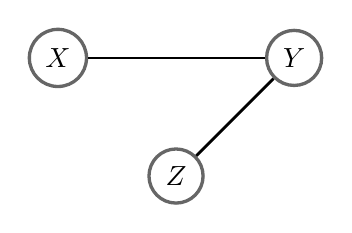
\begin{tikzpicture}[
node/.style={circle, draw=black!60, fill=green!0, very thick, minimum size=5mm,align=center},
]
\node[node] (X) at(0,0) {$X$};
\node[node] (Z) at(1.5,-1.5) {$Z$};
\node[node] (Y) at(3,0) {$Y$};
\draw[-,d] (X) -- (Y);
\draw[-,d] (Y) -- (Z);
\end{tikzpicture}
\end{subfigure}%
\begin{subfigure}{0.3\textwidth}
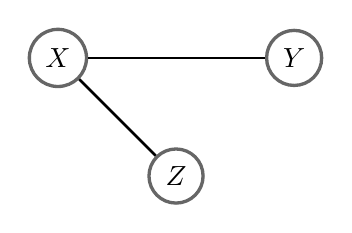
\begin{tikzpicture}[
node/.style={circle, draw=black!60, fill=green!0, very thick, minimum size=5mm,align=center},
]
\node[node] (X) at(0,0) {$X$};
\node[node] (Z) at(1.5,-1.5) {$Z$};
\node[node] (Y) at(3,0) {$Y$};
\draw[-,d] (X) -- (Y);
\draw[-,d] (X) -- (Z);
\end{tikzpicture}
\end{subfigure}
\begin{subfigure}{0.3\textwidth}%
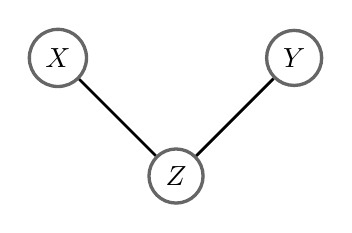
\begin{tikzpicture}[
node/.style={circle, draw=black!60, fill=green!0, very thick, minimum size=5mm,align=center},
]
\node[node] (X) at(0,0) {$X$};
\node[node] (Z) at(1.5,-1.5) {$Z$};
\node[node] (Y) at(3,0) {$Y$};
\draw[-,d] (Y) -- (Z);
\draw[-,d] (X) -- (Z);
\end{tikzpicture}
\end{subfigure}
\caption{If any two edges are present in a graphical model on three nodes then the graph is connected, and thus the joint distribution $\mathbb{P}_{XYZ}$ does not factorise. \label{fig:pairwisejoint}}
\end{figure}



This gives us a statistical test for testing joint dependence. We test each of the three hypotheses:

\begin{align*}
\mathcal{H}_{XY}: \quad \mathbb{P}_{XY } &= \mathbb{P}_{X}\mathbb{P}_{Y}\\
\mathcal{H}_{XZ}: \quad \mathbb{P}_{XZ } &= \mathbb{P}_{X}\mathbb{P}_{Z}\\
\mathcal{H}_{YZ}: \quad \mathbb{P}_{YZ } &= \mathbb{P}_{Y}\mathbb{P}_{Z}\\
\end{align*}

using HSIC. If we reject any two of them, we conclude that the distribution does not factorise. In the remainder of this section, we will call this the Pairwise HSIC test.

\subsubsection{The `3-way HSIC' test}

Recall that in the Lancaster test, our null hypothesis $\mathcal{H}_0$ is a \emph{composite} hypothesis. Let us denote by $\mathcal{H}_X$ the hypothesis that $X \independent (Y,Z)$, and define similarly  $\mathcal{H}_Y$ and  $\mathcal{H}_Z$. Then

\[ \mathcal{H}_0 =  \mathcal{H}_X \lor \mathcal{H}_Y \lor \mathcal{H}_Z \]

and so we reject $\mathcal{H}_0$ if and only if we reject each of $\mathcal{H}_X$, $\mathcal{H}_Y$ and  $\mathcal{H}_Z$. Instead of using the Lancaster statistic to test each of these sub-hypotheses, we could use HSIC:

We can consider $(Y,Z)$ to be a single random variable. We can thus test $\mathcal{H}_X$ (ie whether $(Y,Z)$ is independent of $X$ or not) using HSIC. We can similarly test $\mathcal{H}_Y$ and $\mathcal{H}_Z$. If we reject all three of the sub-hypotheses, we reject $\mathcal{H}_0$. 

We will refer to this test as the 3-way HSIC test throughout the remainder of this section.


\subsection{Multiple testing correction}

When performing multiple hypothesis tests, we must take into consideration the fact that the probability of falsely rejecting one of the hypotheses grows as we increase the number of tests. In both the Lancaster and HSIC-based tests, our null hypothesis consists of multiple sub-hypotheses. In order to control the overall Type-I error rate, we must consider carefully the threshold p-values we use for each of the sub-tests.

\subsubsection{Holm-Bonferroni}


Given a family of multiple hypotheses $\mathcal{H}_1,\mathcal{H}_2,\ldots ,\mathcal{H}_m$, the \emph{Holm-Bonferroni} method \cite{holm1979simple} is a way to control the \emph{family-wise error rate}. This is the probability that one or more of the hypotheses are falsely rejected. To ensure a family-wise error rate of at most $\alpha$, we perform the following procedure.

\begin{enumerate}
\item Let $p_1,\ldots,p_m$ be the p-values corresponding to each hypothesis.
\item Sort the p-values from lowest to highest. Write them as  $p_{(1)},\ldots ,p_{(m)}$ and let $\mathcal{H}_{(1)},\ldots,\mathcal{H}_{(m)}$ be the corresponding hypotheses.
\item Let $k$ be the minimal index such that $p_{(k)} > \frac{\alpha}{m+1-k}$
\item Reject the hypotheses $\mathcal{H}_{(1)},\ldots ,\mathcal{H}_{(k-1)}$ and do not reject the hypotheses $\mathcal{H}_{(k)},\ldots ,\mathcal{H}_{(m)}$. If $k=1$, we reject all of the hypotheses.
\end{enumerate}

\subsubsection{Multiple correction for Pairwise HSIC test}

Observe that we are testing three hypotheses. If we reject any two of the hypotheses, we conclude that the joint distribution $\mathbb{P}_{XYZ}$ does not factorise. How can we bound the Type I error rate of our overall test? Let us consider the following example.

\begin{example}[See Figure \ref{fig:example}]


Suppose that $\mathbb{P}_{XYZ} = \mathbb{P}_{XY}\mathbb{P}_{Z}$, and that $\mathbb{P}_{XY}$ does not factorise. First note that we should reject $\mathcal{H}_{XY}$ but not reject the null hypothesis overall. Suppose however that we falsely reject one of $\mathcal{H}_{YZ}$ or $\mathcal{H}_{XZ}$.  In this case the overall result would be to incorrectly conclude that $\mathbb{P}_{XYZ}$ must not factorise.
\end{example}



\begin{figure}
\centering
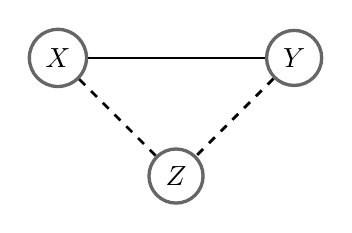
\begin{tikzpicture}[
node/.style={circle, draw=black!60, fill=green!0, very thick, minimum size=5mm,align=center},
]
\node[node] (X) at(0,0) {$X$};
\node[node] (Z) at(1.5,-1.5) {$Z$};
\node[node] (Y) at(3,0) {$Y$};
\draw[-,d] (X) -- (Y);
\draw[-,d,dashed] (Y) -- (Z);
\draw[-,d,dashed] (X) -- (Z);
\end{tikzpicture}
\caption{If we correctly detect the edge XY, but falsely detect edges XZ or YZ, then we would incorrectly conclude that the joint distribution does not factorise.\label{fig:example}}
\end{figure}

Therefore, if our aim is to bound the probability of a Type I error overall by $\alpha$, then we should apply the Holm-Bonferroni method to account for multiple testing error, since the family-wise error rate (ie the probability of incorrectly rejecting at least one of the hypotheses) is what we need to bound, as illustrated by the above example.

\subsubsection{Multiple correction for Lancaster and 3-way HSIC test}

Recall that in the Lancaster and 3-way HSIC tests, our null hypothesis $\mathcal{H}_0$ is a \emph{composite} hypothesis:

\[ \mathcal{H}_0 =  \mathcal{H}_X \lor \mathcal{H}_Y \lor \mathcal{H}_Z \]

where $\mathcal{H}_X$ the hypothesis that $X \independent (Y,Z)$, and $\mathcal{H}_Y$ and $\mathcal{H}_Z$ are defined similarly.

We perform statistical tests for each of $\mathcal{H}_X$, $\mathcal{H}_Y$ and $\mathcal{H}_Z$, and we reject $\mathcal{H}_0$ if and only if we reject each of its components.

We wish to control the Type I error of the composite test - that is, we wish to control the probability of falsely rejecting $\mathcal{H}_0$.  Denote by $A_*$ the event that we reject $\mathcal{H}_*$. Then

\[ \mathbb{P}(A_0) = \mathbb{P}(A_X \land A_Y \land A_Z) \leq \min\{\mathbb{P}(A_X),\mathbb{P}(A_Y), \mathbb{P}(A_Z) \} \]

Whether or not there exists a better bound than this that holds in absolute generality is not clear, because the events $A_X, A_Y$ and $A_Z$ are not independent. If $\mathcal{H}_0$ is true, then at least one of $\mathcal{H}_X$, $\mathcal{H}_Y$ and $\mathcal{H}_Z$ must be true. Therefore, if we use a threshold p-value of $\alpha$ in each statistical test separately, then WLOG assuming that $\mathcal{H}_X$ is true, we see that 

\[ \mathbb{P}(A_0)  \leq \min\{\mathbb{P}(A_X),\mathbb{P}(A_Y), \mathbb{P}(A_Z) \} \leq \mathbb{P}(A_X) = \alpha \]

To conclude: we can bound the Type I error rate by $\alpha$ by setting the Type I error rate for each constituent test individually to be $\alpha$. We refer to this correction as the \emph{`naive' correction} throughout the remainder of this thesis.

In \cite{sejdinovic2013kernel}, it is suggested that one use the Holm-Bonferroni method to control the Type I error rate. This results in a worse test power than the `naive' correction, since it provides overly conservative bounds on the Type I error rate. Indeed, for a rejection of the null to occur using the Holm-Bonferroni correction, the sorted p-values of the hypotheses would have to be lower than $[\frac{\alpha}{3}, \frac{\alpha}{2}, \alpha]$, compared to only $[\alpha, \alpha, \alpha]$ using the method described above.

See Example 3 below for an empirical comparison of the Type I error rates of the two methods on artificial data for which the ground truth is that $\mathcal{H}_0$ is true.

\subsection{Results}
%We perform the tests on three examples of artificial data and two examples of real financial data. We describe the results here. In the following section we will discuss them in more detail.


\subsubsection{Example 1: Artificial data}
Artificial data were generated from autoregressive processes $X$, $Y$ and $Z$ according to:

\begin{align*}
X_t &= \frac{1}{2}X_{t-1} + \epsilon_t\\
Y_t &= \frac{1}{2}Y_{t-1} + \eta_t\\
Z_t &= \frac{1}{2}Z_{t-1} + d(X_t + Y_t) + \zeta_t\\
\end{align*}

where $X_0, Y_0, Z_0, \epsilon_t, \eta_t$ and $\zeta_t$ are \emph{iid} $\mathcal{N}(0,1)$ random variables and $d\in\mathbb{R}$, called the \emph{dependence} coefficient, determines the extent to which the process $(Z_t)_t$ is dependent on $(X_t,Y_t)_t$.

Data were generated according to this definition with varying values for the dependence coefficient. For each value of the dependence coefficient, 500 datasets were generated, each consisting of 2000 consecutive observations of the variables. We ran the Wild Bootstrap with 250 bootstrapping procedures and we used a Gaussian kernel with bandwidth parameter 1 on each of $X$, $Y$ and $Z$.

In this example, the ground truth is that $Z$ is dependent on both $X$ and $Y$ separately, as well as on them both jointly (ie dependent on $(X,Y)$). The results are presented in Figure \ref{fig:ex1}. Observe that the HSIC-based test is able to detect the dependence more easily than the Lancaster test when the interaction is weak, and that when using the `naive' correction, the Lancaster test has a higher test power than when using the Holm-Bonferroni correction.


\begin{figure}[htbp]
  \centering
  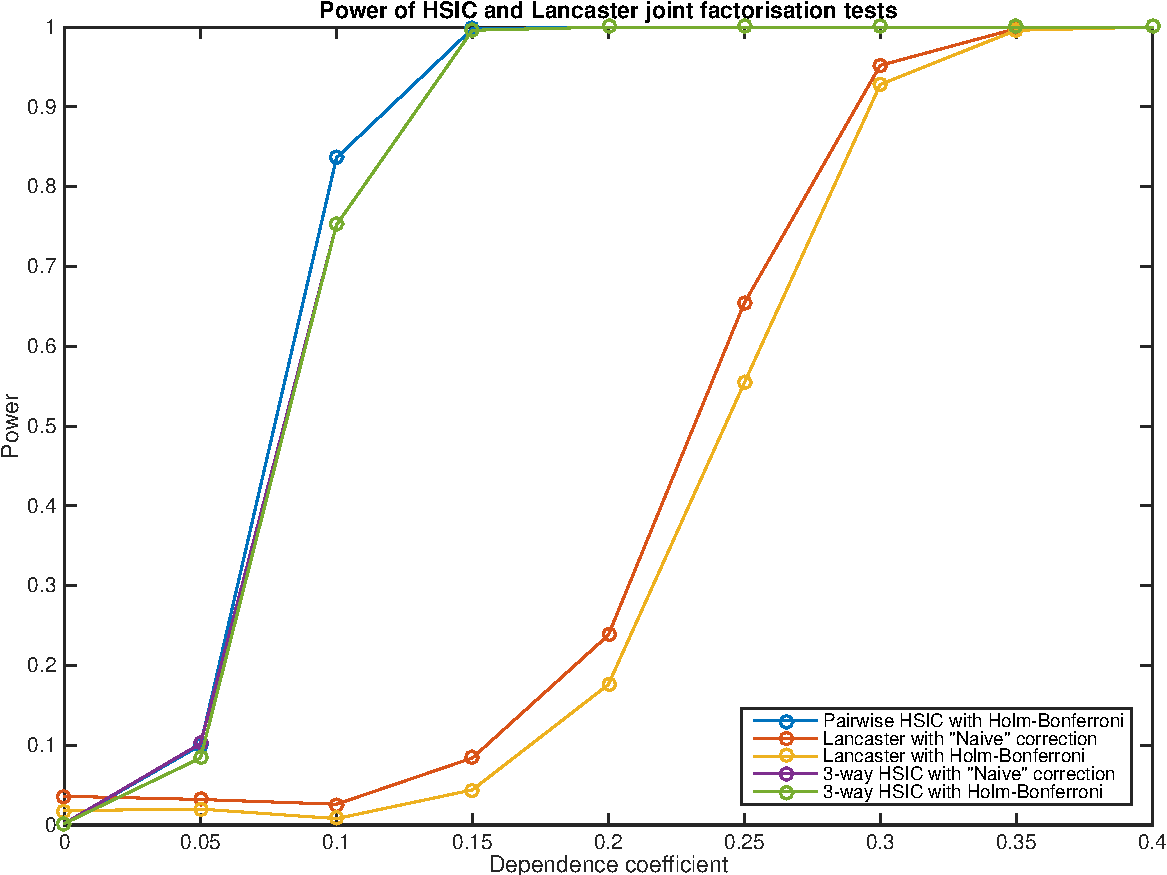
\includegraphics[width=\textwidth]{LancasterBootstrap/code/figures/Example9script_with3HSIC.pdf}
  \caption{Performance of Lancaster and HSIC-based joint dependence tests on data from Example 1. Observe that the HSIC-based tests outperform the Lancaster tests, and that Lancaster with `naive' correction performs better than with Holm-Bonferroni.}
  \label{fig:ex1}
\end{figure}

\subsubsection{Example 2: Artificial data}
Artificial data were generated from autoregressive processes $X$, $Y$ and $Z$ according to:

\begin{align*}
X_t &= \frac{1}{2}X_{t-1} + \epsilon_t\\
Y_t &= \frac{1}{2}Y_{t-1} + \eta_t\\
Z_t &= \frac{1}{2}Z_{t-1} + d |\theta_t|\text{sign}(X_t Y_t) + \zeta_t\\
\end{align*}

where $X_0, Y_0, Z_0, \epsilon_t, \eta_t, \theta_t$ and $\zeta_t$ are \emph{iid} $\mathcal{N}(0,1)$ random variables and $d\in\mathbb{R}$, called the \emph{dependence} coefficient, determines the extent to which the process $(Z_t)_t$ is dependent on $(X_t,Y_t)_t$.

Data were generated according to this definition with varying values for the dependence coefficient. For each value of the dependence coefficient, 500 datasets were generated, each consisting of 2000 consecutive observations of the variables. We ran the Wild Bootstrap with 250 bootstrapping procedures and we used a Gaussian kernel with bandwidth parameter 1 on each of $X$, $Y$ and $Z$.

In contrast to the dataset in Example 1, $Z$ is dependent on the process $(X,Y)$ but is independent of $X$ and $Y$ when considered separately. Indeed, observe that the marginal distributions of $X$ and $Y$ are both normal distributions with mean 0, and thus $\text{sign}(X_t Y_t)$ is either $-1$ or $1$ with equal probability, conditioned upon neither or exactly one of $X_t$ or $Y_t$.

The results are presented in Figure \ref{fig:ex2}. Observe that Pairwise HSIC is unable to correctly identify that the distribution does not factorise. This is because it only looks at the variables pairwise, and so is unable to detect the three-way dependence that Lancaster can detect.

3-way HSIC should in principle be able to detect the dependence, but when the dependence coefficient is low the interactions between $X$ and $(Y,Z)$, as well as between $Y$ and $(X,Z)$, may be very weak.

As before, Lancaster with the `naive' correction outperforms Lancaster with Holm-Bonferroni.

\begin{figure}[htbp]
  \centering
  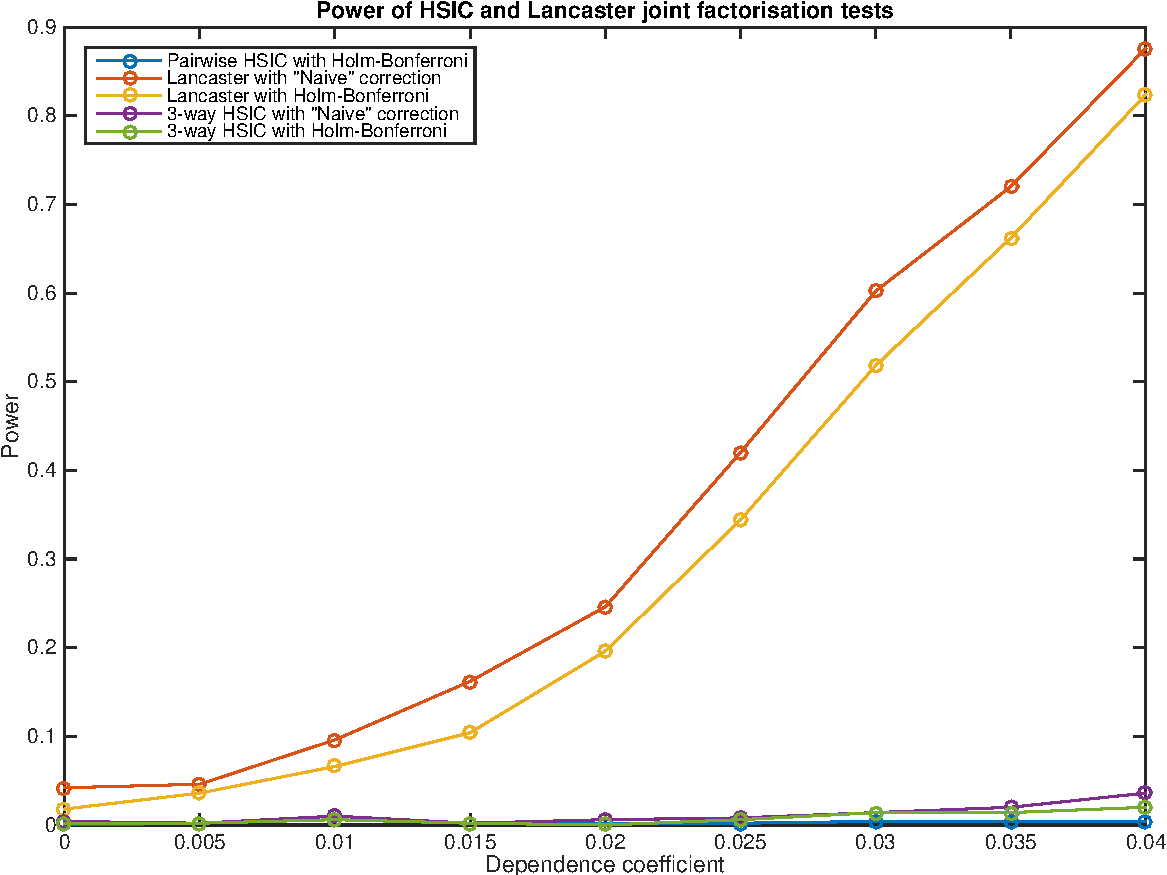
\includegraphics[width=\textwidth]{LancasterBootstrap/code/figures/Example10script_with3HSIC.pdf}
  \caption{Performance of Lancaster and HSIC-based joint dependence tests on data from Example 2. Observe that the Pairwise HSIC does not detect any dependence at all. In the range of dependence coefficients considered, 3-way HSIC appears to be unable to detect dependence whereas Lancaster performs well. Note again that Lancaster with `naive' correction performs better than with Holm-Bonferroni.}
  \label{fig:ex2}
\end{figure}

\subsubsection{Example 3: Artificial data}

The purpose of this example is to understand how the tests behave when the null hypothesis is true, and how well we can control the Type I error rates. 

Artificial data were generated from autoregressive processes $X$, $Y$ and $Z$ according to:

\begin{align*}
X_t &= \frac{1}{2}X_{t-1} + \epsilon_t\\
Y_t &= \frac{1}{2}Y_{t-1} + \eta_t\\
Z_t &= \frac{1}{2}Z_{t-1} + \frac{1}{2}X_{t} + \zeta_t\\
\end{align*}

where $X_0, Y_0, Z_0, \epsilon_t, \eta_t$ and $\zeta_t$ are \emph{iid} $\mathcal{N}(0,1)$ random variables. Observe that  $(X,Z) \independent Y$, and so the null hypothesis is true.

4000 datasets were generated according to this definition, each consisting of 2000 consecutive observations of the variables. We ran the Wild Bootstrap with 250 bootstrapping procedures and we used a Gaussian kernel with bandwidth parameter 1 on each of $X$, $Y$ and $Z$. For each test, the p-values were recorded. For any desired Type I error rate $\alpha$, the proportion of tests that would have resulted in a rejection of the null could then be calculated. This is presented in Figure \ref{fig:ex3}.

Ideally, we would have an empirical Type I error that is very close to, but bounded by, $\alpha$. In this case, we have a good understanding of the Type I error and therefore can choose a threshold in an informed way to control the tradeoff between sensitivity and specificity. It is `bad' if the empirical Type I error is drastically less than the desired level, as this means that the sensitivity of the test is lower than it would otherwise be\footnote{It is `even worse' if the empirical Type I error is not bounded by the desired level. In this case, it is not possible to control the false positive rate! It is for this reason that the Wild Bootstrap is needed, rather than using the permutation bootstrap that works in the \emph{iid case}. See Example 4.}.

Observe that for 3-way HSIC, the empirical Type I error rate is almost exactly as desired. For Pairwise-HSIC, the empirical Type I error rate is slightly less than the desired level. The Lancaster tests have a much lower empirical Type I error than desired. Using the `naive' correction gives a considerable improvement over the Holm-Bonferroni correction, though it is still significantly lower than the desired error.



\begin{figure}[htbp]
  \centering
  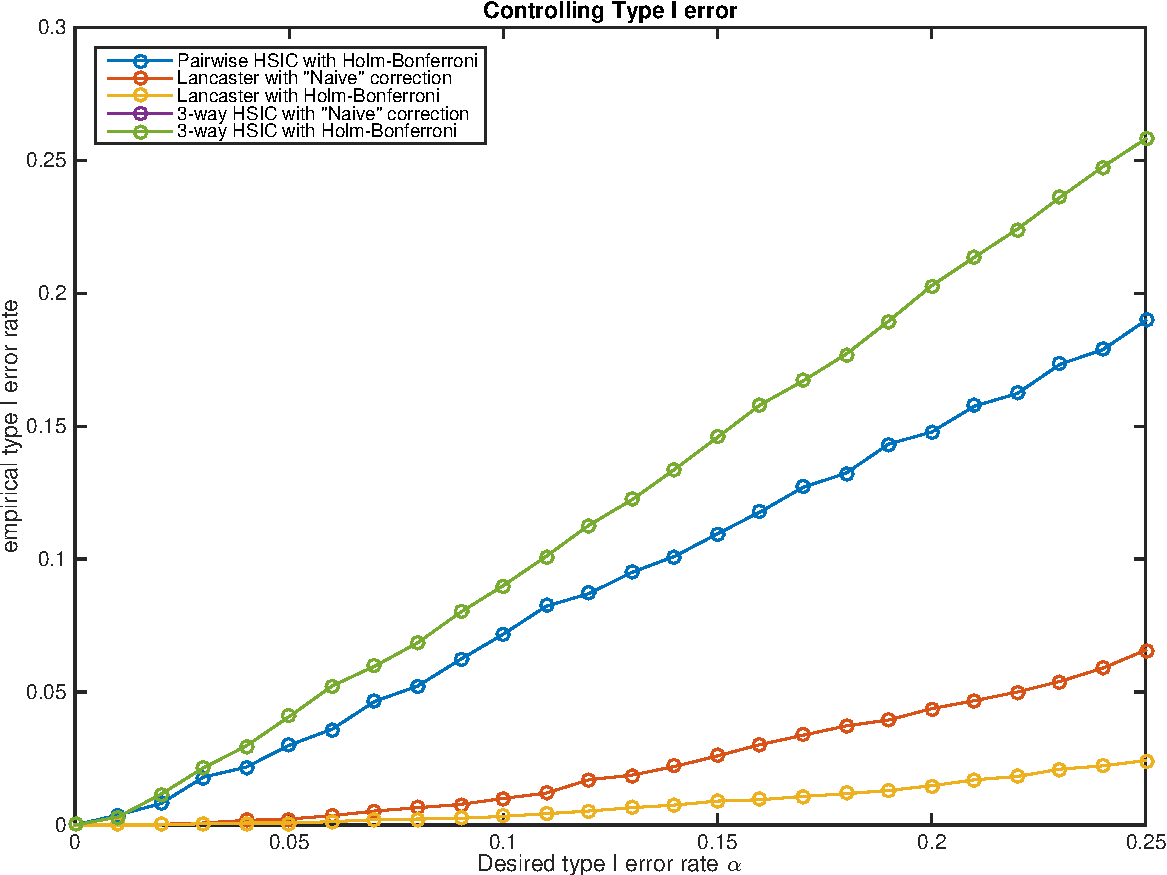
\includegraphics[width=\textwidth]{LancasterBootstrap/code/figures/TypeIErrorExample11_with3HSIC.pdf}
  \caption{Performance of Lancaster and HSIC-based joint dependence tests on data from Example 3. Here the null hypothesis is true, and we measure the empirical Type I error rate as a function of the desired Type I error rate. Observe that 3-way HSIC achieves the desired Type I error rate more or less exactly. Note that using Holm-Bonferroni or the `naive' correction seemingly makes no difference for 3-way HSIC - indeed, the purple line is not visible as it is perfectly obscured by the green line. Pairwise HSIC is also close to the desired error. Note that for Lancaster, using the `naive' rather than Holm-Bonferroni correction results in a Type I error rate that is closer to the desired rate, thus implying that this correction gives a better test power.}
  \label{fig:ex3}
\end{figure}

\subsubsection{Example 4: Artificial data}

The purpose of this example is to demonstrate that the Wild Bootstrap is actually needed when resampling from the null distribution.

Artificial data generated from autoregressive processes $X$, $Y$ and $Z$ according to:

\begin{align*}
X_t &= aX_{t-1} + \epsilon_t\\
Y_t &= aY_{t-1} + \eta_t\\
Z_t &= aZ_{t-1} +  \zeta_t\\
\end{align*}

where $X_0, Y_0, Z_0, \epsilon_t, \eta_t$ and $\zeta_t$ are \emph{iid} $\mathcal{N}(0,1)$ random variables and $a$, called the \emph{dependence coefficient}, determines how temporally dependent the processes are. Observe that each process is independent of the others and so the null hypothesis is true.

We performed the Lancaster test using both the Wild Bootstrap and simple permutation bootstrap (used in the \emph{iid} case) methods to sample from the null distribution. We used a fixed desired false positive rate $\alpha = 0.05$ with sample of size 1000, with 500 experiments run for each value of $a$. Figure \ref{fig:wbnec} shows the false positive rates for these two methods for varying $a$. It shows that as the processes become more dependent, the false positive rate for the permutation method becomes very large, and is not bounded by the fixed $\alpha$, whereas the false positive rate for the Wild Bootstrap method is bounded by $\alpha$.

\begin{figure}[htbp]
  \centering
  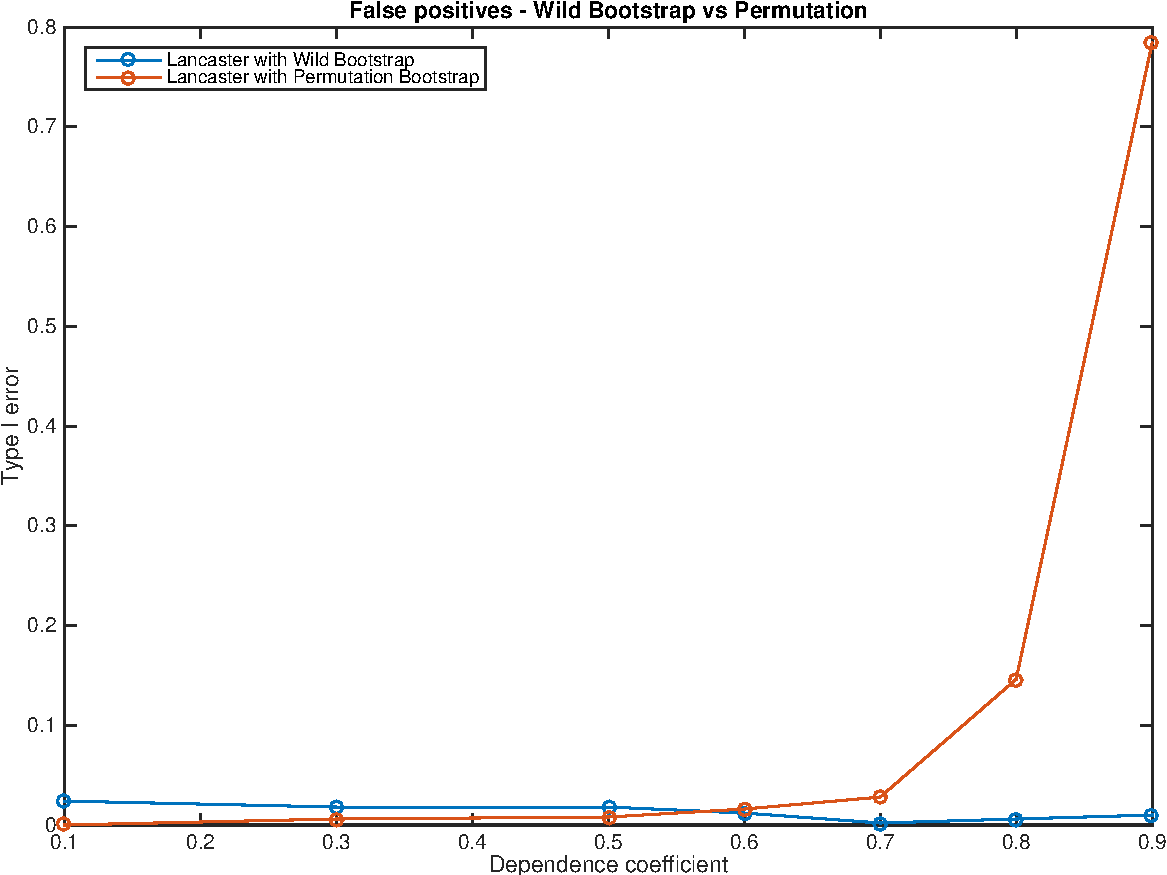
\includegraphics[width=\textwidth]{LancasterBootstrap/code/figures/wildBootstrap_is_necessary.pdf}
  \caption{Empirical Type I errors of the Lancaster test when using the Wild Bootstrap and simple permutation bootstrap methods. Observe that when the dependence coefficient is large, a very large false positive rate is obtained when using the permutation bootstrap. This implies that the Wild Bootstrap is indeed actually needed - the permutation bootstrap does not work in this example.}
  \label{fig:wbnec}
\end{figure}

\subsubsection{Example 5: Forex data}

We performed the tests on exchange rates CHF/USD, CHF/GBP and USD/CAD from 01/01/1990 until 31/12/1999. We tried to answer two questions using this data:

\begin{enumerate}[(i)]
\item Are the exchange rates themselves dependent?
\item Are the fluctuations within each time series dependent?
\end{enumerate}

We performed two different types of preprocessing before running the tests.

To answer (i), we took logarithms of each datum, then centred each time series with respect to its mean and then scaled each time series to have unit variance. We refer to these processed time series as the normalised time series. Figure \ref{fig:ex4_processed} displays the normalised time series. Observe that these time series do not appear to be stationary, and so application of the Wild Bootstrap may not be valid.

To answer (ii), we first took logarithms of each datum. We then smoothened each time series by taking a 5-day running average, and subtracted these from the original time series. We then centred and scaled these `fluctuation time series' to each have zero mean and unit variance. Figure \ref{fig:ex4_fluctuations} shows the fluctuation time series after this procedure.


\begin{figure}[htbp]
  \centering
  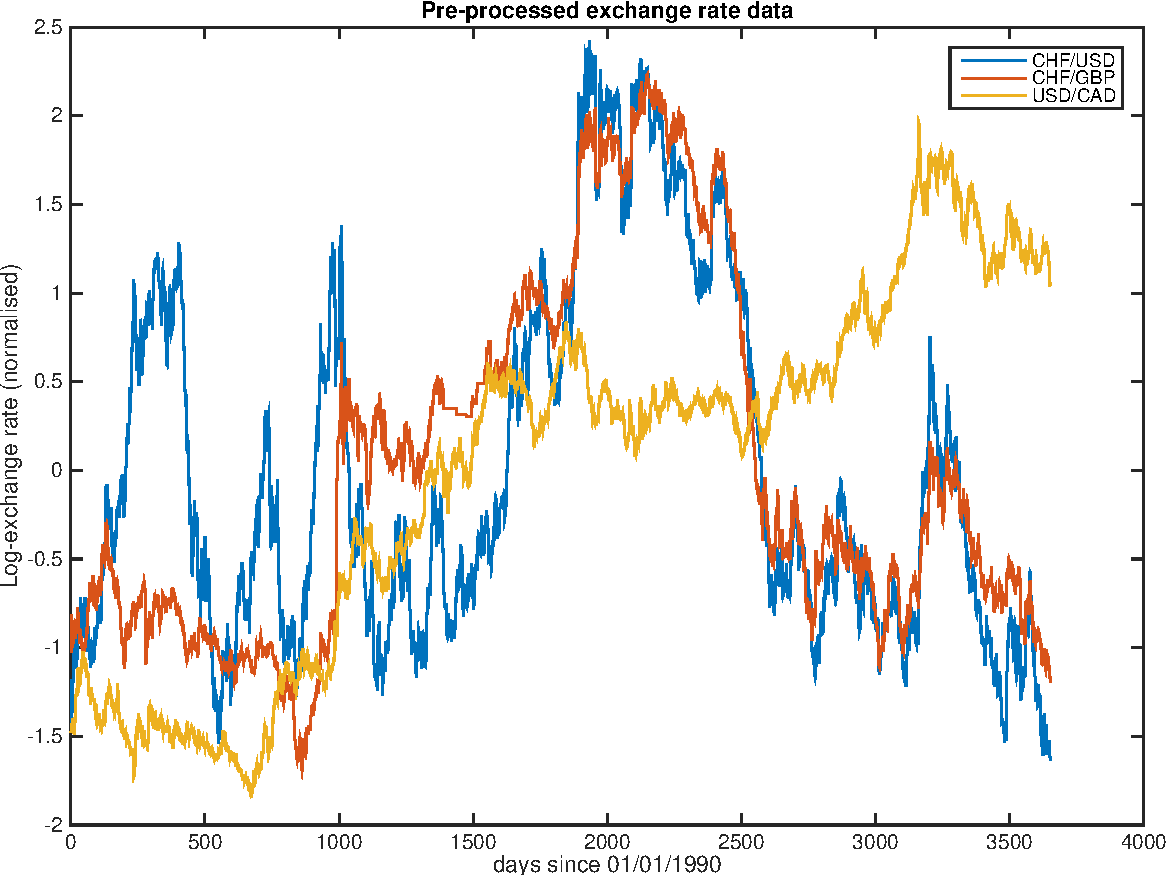
\includegraphics[width=\textwidth]{LancasterBootstrap/code/figures/real_data_example_normalised_data.pdf}
  \caption{Normalised time series for data in Example 5. Observe that these time series do not appear to be stationary, and so application of the Wild Bootstrap may not be valid.}
  \label{fig:ex4_processed}
\end{figure}

\begin{figure}[htbp]
  \centering
  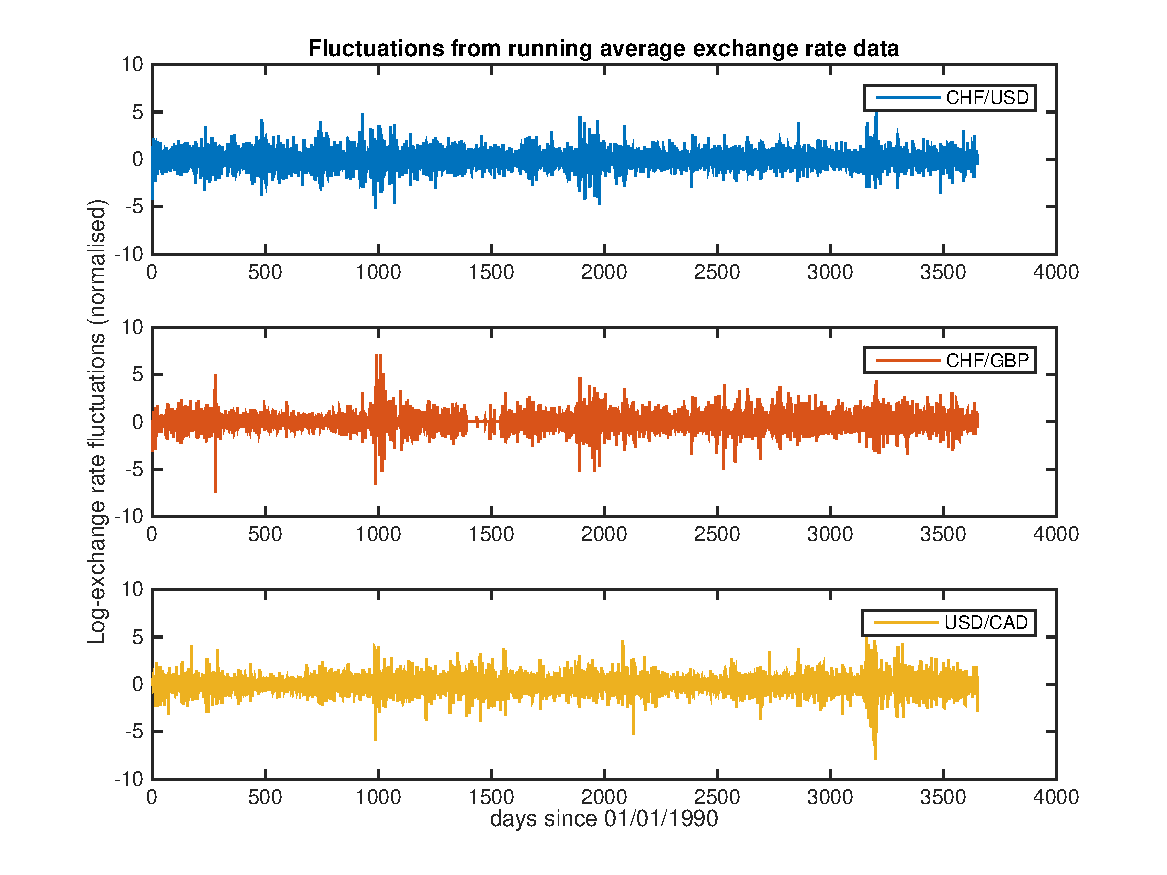
\includegraphics[width=\textwidth]{LancasterBootstrap/code/figures/real_data_example_fluctuations.pdf}
  \caption{Fluctuation time series for data in Example 5.}
  \label{fig:ex4_fluctuations}
\end{figure}

For the output of the code when run on these datasets, see the appendix. For the normalised data, both the HSIC-based tests and the Lancaster test (with both `naive' and Holm-Bonferroni corrections) rejected the null hypothesis (ie the joint distribution does not factorise). For the fluctuation data, the HSIC tests rejected the null hypothesis, however Lancaster failed to reject the null hypothesis.


\subsubsection{Example 6: Forex data}

We performed the tests on exchange rates GBP/USD, USD/HRK and GBP/HRK for 4534 working days days from 09/09/1996. We tried to answer the same questions as in Example 5 and so processed the data in the same way. Figure \ref{fig:ex5_processed} displays the normalised time series. Figure \ref{fig:ex5_fluctuations} displays the fluctuation time series. Note that the time series in Figure \ref{fig:ex5_processed} do not appear to be stationary and so application of the Wild Bootstrap may not be valid.


\begin{figure}[htbp]
  \centering
  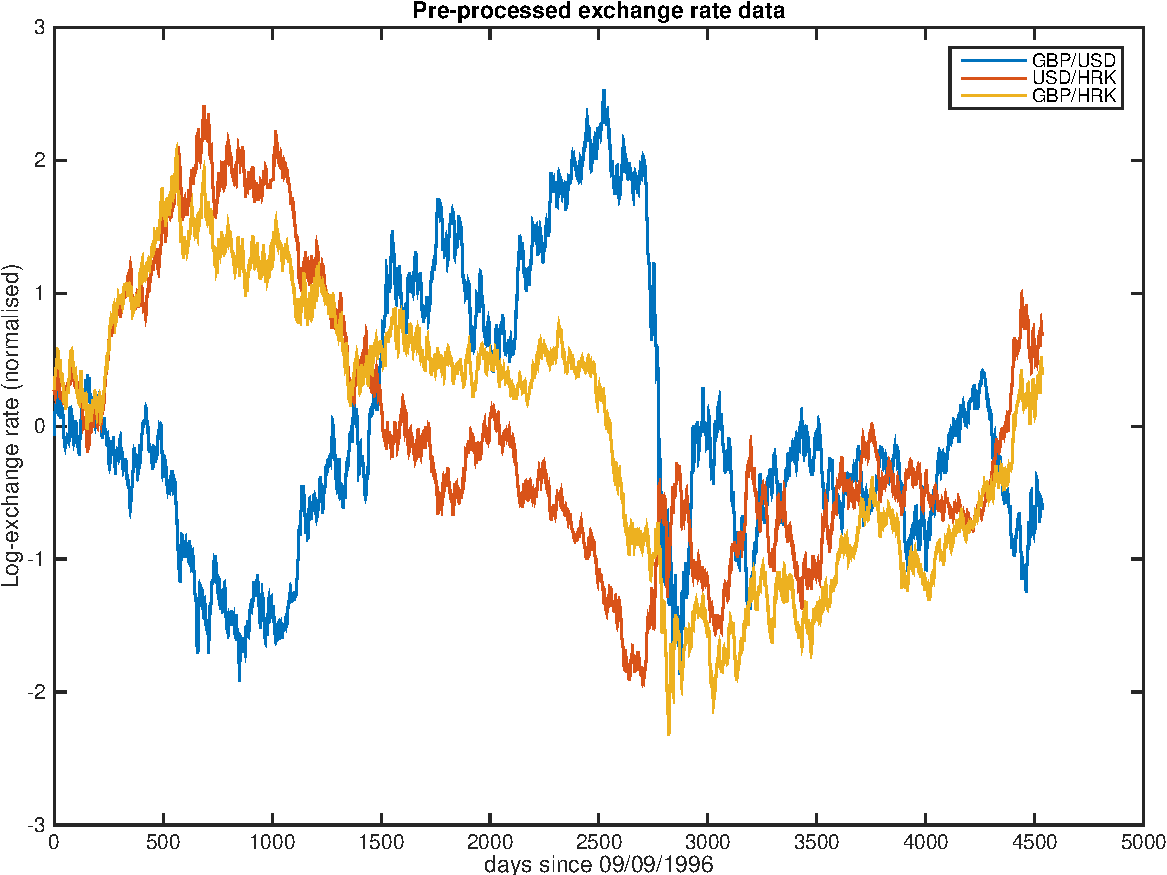
\includegraphics[width=\textwidth]{LancasterBootstrap/code/figures/real_data_example2_normalised_data.pdf}
  \caption{Normalised time series for data in Example 6. Observe that these time series do not appear to be stationary, and so application of the Wild Bootstrap may not be valid.}
  \label{fig:ex5_processed}
\end{figure}

\begin{figure}[htbp]
  \centering
  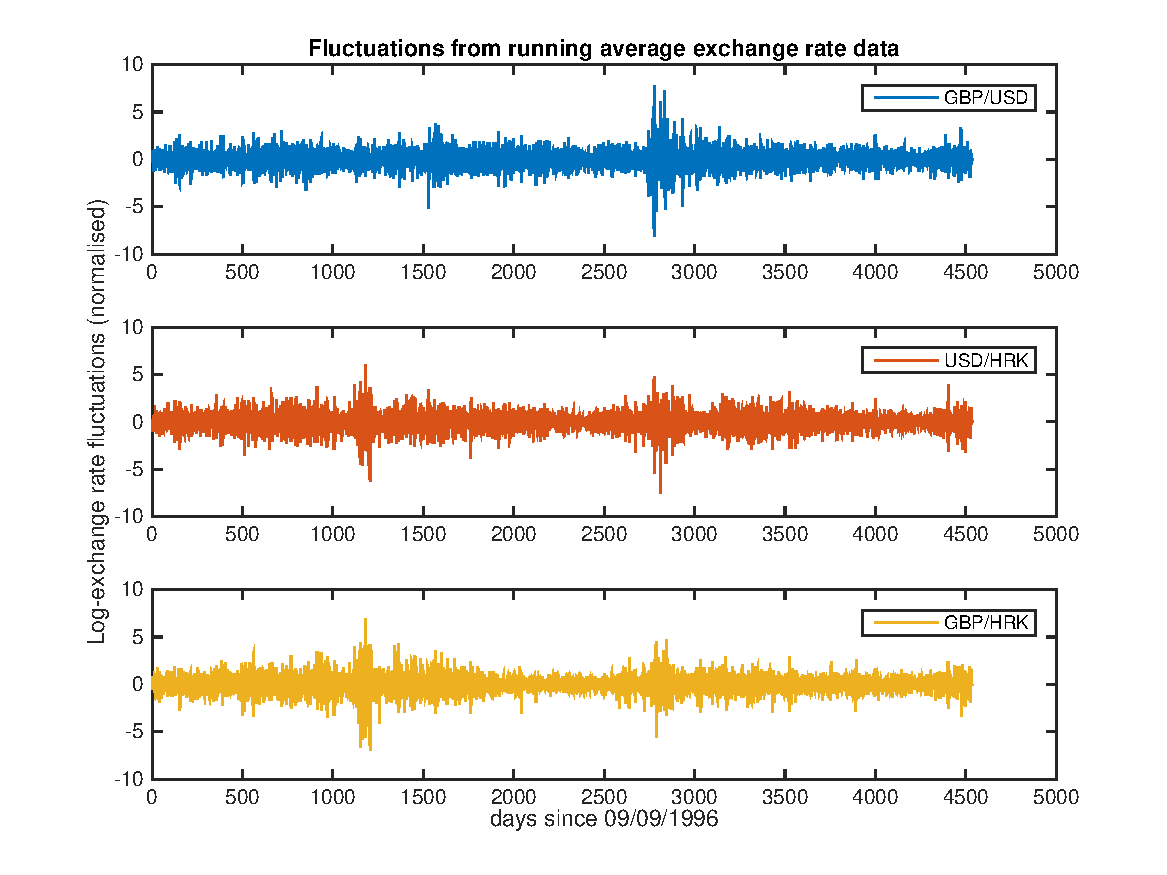
\includegraphics[width=\textwidth]{LancasterBootstrap/code/figures/real_data_example2_fluctuations.pdf}
  \caption{Fluctuation time series for data in Example 6.}
  \label{fig:ex5_fluctuations}
\end{figure}

For the output of the code when run on these datasets, see the appendix. For both sets of processed data, all of the tests reject the null hypothesis (ie they detect that the distribution does not factorise and thus the variables are all dependent).


\subsection{Discussion of results}

%\begin{itemize}
%\item Lancaster can detect dependence in some circumstances for which HSIC-based test fails
%\item When dependence is pairwise, HSIC is better
%\item The false positive rate for Lancaster is harder to control. This may account for some of the fact that HSIC is better, as this may just be a consequence of the increased specificity implying a decreased specificity (power).
%\item Naive correction is better than holm bonferroni.
%\item Looking at the real data, we see the same story. In example 4, the HSIC based test picks up on dependence that the Lancaster test is not able to detect. Note however though that Lancaster works on example 5. Observe that in example 5, any two exchange rates should determine the third because of arbitrage - thus there is very strong 3-way dependence that is not present in example 4.
%\item we should however take the analysis of the real data with a pinch of salt, particularly the normalised data as we cannot know whether the data fulfill the requirements of the wild bootstrap.
%\end{itemize}

Let us note first that the Lancaster test can detect dependence in some circumstances for which the HSIC-based tests fail to detect dependence, such as in Example 2. This is an example of a situation in which $Z$ is weakly dependent on $X$ and $Y$ separately, but strongly dependent on the pair $(X,Y)$. 

In cases for which the pairwise dependence is strong, it appears that the HSIC-based tests have a better power than the Lancaster test, as demonstrated by Example 1.

There is a confounding factor here though - as demonstrated by Example 3, the Type I error of the Lancaster test has a much cruder bound than those for Pairwise HSIC and 3-way HSIC. It may be possible that the lower power of the Lancaster test is due, at least in part, to the fact that we are setting our thresholds for the p-values to be too low with the result that we fail to reject too many cases in which the null hypothesis in fact does not hold.

Examples 1, 2 and 3 together serve to demonstrate that the `naive' multiple testing correction is better than the previously proposed Holm-Bonferroni correction in \cite{sejdinovic2013kernel}. This improvement should hold in the \emph{iid} case considered in \cite{sejdinovic2013kernel} too.

Looking at the real data analysed in Examples 5 and 6, we see that the Lancaster test did not allow us to draw any conclusions beyond what we learned from the HSIC-based tests, however it is possible that it may be useful beyond HSIC in other circumstances. One `problem' with financial data is that there are many confounding factors, and so it is in general quite hard to find pairs of variables that are marginally independent of one another (or weakly dependent) and yet (strongly) dependent via a third - these are the situations in which the Lancaster test is particularly useful. 

It is worth nothing that the Lancaster test performs well on the data in Example 6 - here there are good reasons to believe that there is a very strong 3-way dependence between the three random variables under consideration, beyond the dependence found between pairs of variables. Indeed, since the three variables cover all exchange rates between three currencies, any two should determine the third (since trading, for example, GBP $\longrightarrow$ USD  $\longrightarrow$ HRK  $\longrightarrow$ GBP should result in no net loss or gain, else there would be opportunity for arbitrage).

It should be noted that it is not clear whether the time series used in Examples 5 and 6 satisfy the conditions required of the Wild Bootstrap. `By eye' inspection suggests that stationarity does not hold in the normalised time series. Whether or not the $\beta$- and $\tau$-mixing conditions hold in either the normalised time series or the fluctation timeseries is unclear.

\newpage
\section{Conclusions and directions for further research}

In this thesis we present a kernel statistical test of dependence between three stationary random processes that satisfy $\beta$- and $\tau$-mixing assumptions. The null hypothesis of this test is that the joint distribution $\mathbb{P}_{XYZ}$ factorises in some way, so that rejection of the null implies that $\mathbb{P}_{XYZ}$ does not factorise. This uses the Lancaster interaction as its test statistic, and uses the Wild Bootstrap to resample the statistic under the null distribution. 

In order to show that use of the Wild Bootstrap results in samples from the correct null distribution, we prove that the normalised Lancaster statistic is a degenerate V-statistic under the null hypothesis. This is the main contribution of this thesis. The same proof idea is used to give a new proof that the Wild Bootstrap can be used with HSIC when the observations are drawn from random processes satisfying the same conditions as stated above.

When performing the Lancaster statistical test, we test multiple hypotheses and so consider multiple testing corrections. A minor contribution of this thesis is to show that the existing corrections used were more conservative than necessary, and a new, better correction is provided resulting in a greater test power.

Comparing the performance of the Lancaster test with HSIC-based tests on artificial data shows that, when the three variables interact weakly when considered pairwise, but strongly when considered all together, the Lancaster test outperforms the HSIC-based tests. However, when strong pairwise interactions are present, the HSIC-based tests considered are more able to identify joint dependence. An interesting finding that may account for some of the relatively-better-power of the HSIC-based tests was that even with the better multiple testing correction, the empirical bound on the Type I errors was found to be very severe. Thus, some power of the Lancaster test may be lost due to in practice having a more extreme test statistic threshold than necessary for any given Type I error bound.

Moving forward, there are many questions that this research has raised. We list some here.

\begin{itemize}
\item Recall that the statement of the theorem of the Wild Bootstrap lists three sets of conditions. They concern: (1) Conditions on the observations; (2) Conditions on the test statistic; (3) Conditions on the bootstrapping process. In this thesis we have proved that the Lancaster and HSIC test statistics satisfy (2), but what about the other two conditions? How can we tell if observations satisfy (1)? What happens if we choose a different bootstrap process satisfying (3)?
\item Recall that we use a Hilbert space Central Limit Theorem for random processes in our proof. Currently we assume that they are $\beta$-mixing, in addition to the $\tau$-mixing already needed for the wild bootstrap. Is it possible to relax the conditions on the processes? 
\item Experiment 3 shows that we are bounding the Type I error rate too severely, possibly at the expense of test power. Can we better understand how to bound the false positive rate?
\item When we fail to reject the null hypothesis of the Lancaster test, we cannot conclude anything about the distribution. This is because the Lancaster statistic can be zero \emph{even when the joint distribution does not factorise}. Better understanding these `counterexamples' and possibly even characterising them might help us to create a consistent test of joint dependence on three variables.
\end{itemize}



\newpage
\section{Appendix}

\subsection{Proofs}

\begin{claim}\label{claim:HSICT}
Using the same setup as in Claim \ref{claim:HSICinvariant},

$T(\phi, \psi, \mathcal{D}) = \frac{1}{n^2} (K\circ L)_{++} - \frac{2}{n^3} (KL)_{++} + \frac{1}{n^2} K_{++}L_{++}$
\end{claim}

There are two ways to prove this. The first relies on the Lancaster paper \cite{sejdinovic2013kernel}, and is relatively short. The second is from direct manipulation of the definition of $T$ and is only straightforward, but extremely tedious, algebra.

\begin{claimproof}(i) \emph{Using the results from Lancaster paper}
Noting first by definition of $T$, and then by \emph{Section 4.1} in \cite{sejdinovic2013kernel},

\begin{align*}
T(\phi,\psi,\omega,\mathcal{D}) & = \frac{1}{n^2}(\tilde{K} \circ \tilde{L})_{++}\\
& = \| \hat{P}_{XY} - \hat{P}_X \hat{P}_Y \|_{k\otimes l }^2\\
& = \langle \hat{P}_{XY} ,\hat{P}_{XY} \rangle - 2 \langle \hat{P}_{XY} , \hat{P}_X \hat{P}_Y \rangle + \langle \hat{P}_X \hat{P}_Y, \hat{P}_X \hat{P}_Y\rangle
\end{align*}

Each of these inner products can be expressed in terms of the Gram matrices $K$ and $L$. \emph{Table 1} in \cite{sejdinovic2013kernel}, which has been exactly copied here as Table \ref{tab: 2vartab} for convenience, gives us each of these expressions. Substituting yields the desired result.

\begin{table}
\caption{\label{tab: 2vartab}{\footnotesize $V$-statistic estimates of $\left\langle \left\langle \nu,\nu'\right\rangle \right\rangle _{k\otimes l}$
in the two-variable case. Note that this table has been copied exactly from \cite{sejdinovic2013kernel}, and is not the original work of the author of this thesis}}


\centering{}{\small }%
\begin{tabular}{|c|c|c|}
\hline 
{\small $\nu\backslash\nu'$} & {\small $P_{XY}$} & {\small $P_{X}P_{Y}$}\tabularnewline
\hline 
\hline 
{\small $P_{XY}$} & {\small $\frac{1}{n^{2}}\left(K\circ L\right)_{++}$} & {\small $\frac{1}{n^{3}}\left(KL\right)_{++}$}\tabularnewline
\hline 
{\small $P_{X}P_{Y}$} &  & {\small $\frac{1}{n^{4}}K_{++}L_{++}$}\tabularnewline
\hline 
\end{tabular}
\end{table}

\end{claimproof}


\begin{claimproof} (ii) \emph{A direct proof}
\begin{align*}
& T(\phi, \psi, \mathcal{D})\\
 &=\frac{1}{n^2} \mathlarger{\mathlarger{\sum_{ij}}} \mathlarger{\mathlarger{\langle}} \phi(X_i) - \frac{1}{n}\sum_k \phi(X_k), \phi(X_j) - \frac{1}{n}\sum_k \phi(X_k) \mathlarger{\mathlarger{\rangle}} \\&\quad\quad\quad\quad\quad\quad \times\mathlarger{\mathlarger{\langle}} \psi(Y_i) - \frac{1}{n}\sum_k \psi(Y_k), \psi(Y_j) - \frac{1}{n}\sum_k \psi(Y_k) \mathlarger{\mathlarger{\rangle}} \\
& = \frac{1}{n^2} \mathlarger{\mathlarger{\sum_{ij}}} \mathlarger{\mathlarger{\{}} \langle \phi(X_i),\phi(X_j)\rangle - \frac{1}{n} \sum_k \langle \phi(X_i),\phi(X_k)\rangle\\&\quad\quad\quad\quad\quad\quad - \frac{1}{n} \sum_k \langle \phi(X_k),\phi(X_j)\rangle +\frac{1}{n^2} \sum_{kl} \langle \phi(X_k),\phi(X_l)\rangle   \mathlarger{\mathlarger{\}}} \\
& \quad \times \mathlarger{\mathlarger{\{}} \langle \psi(Y_i),\psi(Y_j)\rangle - \frac{1}{n} \sum_k \langle \psi(Y_i),\psi(Y_k)\rangle - \frac{1}{n} \sum_k \langle \psi(Y_k),\psi(Y_j)\rangle +\frac{1}{n^2} \sum_{kl} \langle \psi(Y_k),\psi(Y_l)\rangle   \mathlarger{\mathlarger{\}}} \\
& = \frac{1}{n^2} \mathlarger{\mathlarger{\sum_{ij}}} \mathlarger{\mathlarger{\{}} K_{ij} - \frac{1}{n} K_{i+} - \frac{1}{n}K_{+j} +\frac{1}{n^2} K_{++}   \mathlarger{\mathlarger{\}}} \mathlarger{\mathlarger{\{}} L_{ij} - \frac{1}{n} L_{i+} - \frac{1}{n}L_{+j} +\frac{1}{n^2} L_{++}   \mathlarger{\mathlarger{\}}} \\ 
& = \frac{1}{n^2} \mathlarger{\mathlarger{\sum_{ij}}} \mathlarger{\mathlarger{\{}} K_{ij} L_{ij} - \frac{1}{n} K_{ij} L_{i+} - \frac{1}{n}K_{ij} L_{+j} +\frac{1}{n^2} K_{ij} L_{++}  \\
& - \frac{1}{n} K_{i+}L_{ij} + \frac{1}{n^2} K_{i+}L_{i+} + \frac{1}{n^2}K_{i+}L_{+j} - \frac{1}{n^3} K_{i+}L_{++}\\
& -  \frac{1}{n}K_{+j}L_{ij} + \frac{1}{n^2}K_{+j} L_{i+} + \frac{1}{n^2}K_{+j} L_{+j} -\frac{1}{n^3} K_{+j} L_{++}\\
& + \frac{1}{n^2} K_{++}L_{ij} - \frac{1}{n^3}K_{++} L_{i+} - \frac{1}{n^3}K_{++}L_{+j} +\frac{1}{n^4}K_{++} L_{++}\\ \\
\end{align*}
\begin{align*}
=& \frac{1}{n^2} \mathlarger{\mathlarger{\{}} 
\sum_{ij} K_{ij}L_{ij} - \frac{1}{n} \sum_i K_{i+}L_{i+} - \frac{1}{n} \sum_j K_{+j}L_{+j} + \frac{1}{n^2}K_{++}L_{++} \\
& \textcolor{blue}{- \frac{1}{n} \sum_i K_{i+}L_{i+} + \frac{1}{n} \sum_iK_{i+}L_{i+}} \textcolor{red}{+ \frac{1}{n^2}K_{++}L_{++} - \frac{1}{n^2} K_{++}L_{++}}\\
& \textcolor{blue}{-  \frac{1}{n}\sum_j K_{+j}L_{+j}} \textcolor{red}{+ \frac{1}{n^2}K_{++} L_{++}}  \textcolor{blue}{+\frac{1}{n}\sum_j K_{+j} L_{+j}} \textcolor{red}{ -\frac{1}{n^2} K_{++} L_{++}}\\
&\textcolor{red}{ + \frac{1}{n^2} K_{++}L_{++} - \frac{1}{n^2}K_{++} L_{++} - \frac{1}{n^2}K_{++}L_{++} + \frac{1}{n^2}K_{++} L_{++}} \mathlarger{\mathlarger{\}}}\\ \\
& = \frac{1}{n^2} (K\circ L)_{++} - \frac{2}{n^3} (KL)_{++} + \frac{1}{n^2} K_{++}L_{++}
\end{align*}
where the last equality follows due to the coloured terms cancelling and the middle two black terms being equal by symmetry of $K$ and $L$.
\end{claimproof}

\begin{claim}\label{claim:LancasterT}
Using the same setup as in Claim \ref{claim:Lancasterinvariant},

\begin{alignat*}{3}
T(\phi,\psi,\omega,\mathcal{D}) &= \frac{1}{n^2}(K \circ L\circ M)_{++} && -
\frac{2}{n^3}((K\circ L) M)_{++} && - 
\frac{2}{n^3}((K \circ M) L)_{++} \\ & - 
\frac{2}{n^3}((M \circ L) K)_{++} && + 
\frac{1}{n^4}(K \circ L)_{++} M_{++} && + 
\frac{1}{n^4}(K \circ M)_{++} L_{++} \\ & + 
\frac{1}{n^4}(L \circ M)_{++} K_{++} && + 
\frac{2}{n^4}(MKL)_{++} && + 
\frac{2}{n^4}(KLM)_{++} \\& + 
\frac{2}{n^4}(KML)_{++} && + 
\frac{4}{n^4}tr(K_+ \circ L_+ \circ M_+) && -
\frac{4}{n^5}(K L)_{++} M_{++} \\ & - 
\frac{4}{n^5}(KM)_{++}L_{++} && - 
\frac{4}{n^5}(LM)_{++} K_{++} && +
\frac{4}{n^6}K_{++} L_{++} M_{++}
\end{alignat*}
\end{claim}


There are two ways to prove this. The first relies on the Lancaster paper \cite{sejdinovic2013kernel}, and is relatively short. The second is from direct manipulation of the definition of $T$ and is only straightforward, but extremely tedious, algebra. The second proof is included to demonstrate that the result \emph{can} be derived from `first principles', without the need for advanced theory, though the author would recommend that the first proof is a much better way of thinking about the problem.

\begin{claimproof}(i) \emph{Using Lancaster interaction paper}

Noting first by definition of $T$, and then by \emph{Proposition 3} in \cite{sejdinovic2013kernel},

\begin{align*}
T(\phi,\psi,\omega,\mathcal{D}) & = \frac{1}{n^2}(\tilde{K} \circ \tilde{L}\circ \tilde{M})_{++}\\
& = \| \Delta_L \hat{P} \|_{k\otimes l \otimes m}^2
\end{align*}


Next, expanding  $ \Delta_L \hat{P}$ in terms of empirical embeddings of various factorisations of the joint, as in equation $(2)$ of \cite{sejdinovic2013kernel} yields

\begin{align*}
\| \Delta_L \hat{P} \|_{k\otimes l \otimes m}^2 &= \| \hat{P}_{XYZ} - \hat{P}_{XY}\hat{P}_{Z} - \hat{P}_{YZ}\hat{P}_{X} - \hat{P}_{XZ}\hat{P}_{Y} + 2\hat{P}_{X}\hat{P}_{Y}\hat{P}_{Z}\|_{k\otimes l \otimes m}^2 \\
& = 
\langle \hat{P}_{XYZ} , \hat{P}_{XYZ} \rangle - 
\langle \hat{P}_{XYZ} , \hat{P}_{XY}\hat{P}_{Z}\rangle - 
\langle \hat{P}_{XYZ} , \hat{P}_{YZ}\hat{P}_{X} \rangle \\ & \quad- 
\langle \hat{P}_{XYZ} , \hat{P}_{XZ}\hat{P}_{Y}\rangle +
2 \langle \hat{P}_{XYZ} ,\hat{P}_{X}\hat{P}_{Y}\hat{P}_{Z} \rangle \\& -
\langle \hat{P}_{XY}\hat{P}_{Z} , \hat{P}_{XYZ} \rangle +
\langle \hat{P}_{XY}\hat{P}_{Z} , \hat{P}_{XY}\hat{P}_{Z}\rangle + 
\langle \hat{P}_{XY}\hat{P}_{Z} , \hat{P}_{YZ}\hat{P}_{X} \rangle \\ & \quad + 
\langle \hat{P}_{XY}\hat{P}_{Z} , \hat{P}_{XZ}\hat{P}_{Y}\rangle -
2 \langle \hat{P}_{XY}\hat{P}_{Z} ,\hat{P}_{X}\hat{P}_{Y}\hat{P}_{Z} \rangle \\& -
\langle \hat{P}_{YZ}\hat{P}_{X} , \hat{P}_{XYZ} \rangle + 
\langle \hat{P}_{YZ}\hat{P}_{X} , \hat{P}_{XY}\hat{P}_{Z}\rangle + 
\langle \hat{P}_{YZ}\hat{P}_{X} , \hat{P}_{YZ}\hat{P}_{X} \rangle \\ & \quad +
\langle \hat{P}_{YZ}\hat{P}_{X} , \hat{P}_{XZ}\hat{P}_{Y}\rangle -
2 \langle \hat{P}_{YZ}\hat{P}_{X} ,\hat{P}_{X}\hat{P}_{Y}\hat{P}_{Z} \rangle \\& -
\langle \hat{P}_{XZ}\hat{P}_{Y} , \hat{P}_{XYZ} \rangle + 
\langle \hat{P}_{XZ}\hat{P}_{Y} , \hat{P}_{XY}\hat{P}_{Z}\rangle +
\langle \hat{P}_{XZ}\hat{P}_{Y} , \hat{P}_{YZ}\hat{P}_{X} \rangle \\ & \quad + 
\langle \hat{P}_{XZ}\hat{P}_{Y} , \hat{P}_{XZ}\hat{P}_{Y}\rangle -
2 \langle \hat{P}_{XZ}\hat{P}_{Y} ,\hat{P}_{X}\hat{P}_{Y}\hat{P}_{Z} \rangle \\& +
2\langle \hat{P}_{X}\hat{P}_{Y}\hat{P}_{Z} , \hat{P}_{XYZ} \rangle - 
2\langle \hat{P}_{X}\hat{P}_{Y}\hat{P}_{Z} , \hat{P}_{XY}\hat{P}_{Z}\rangle - 
2\langle \hat{P}_{X}\hat{P}_{Y}\hat{P}_{Z} , \hat{P}_{YZ}\hat{P}_{X} \rangle \\ & \quad- 
2\langle \hat{P}_{X}\hat{P}_{Y}\hat{P}_{Z} , \hat{P}_{XZ}\hat{P}_{Y}\rangle +
4 \langle \hat{P}_{X}\hat{P}_{Y}\hat{P}_{Z} ,\hat{P}_{X}\hat{P}_{Y}\hat{P}_{Z} \rangle \\& 
\end{align*}

Each of these inner products can be expressed in terms of the Gram matrices $K$, $L$ and $M$. \emph{Table 2} in \cite{sejdinovic2013kernel}, which has been exactly copied here as Table \ref{tab: 3vartab} for convenience, gives us each of these expressions. Substituting yields the desired result.


\begin{table}
\caption{\label{tab: 3vartab}{\footnotesize $V$-statistic estimates of $\left\langle \left\langle \nu,\nu'\right\rangle \right\rangle _{k\otimes l\otimes m}$
in the three-variable case. Note that this table has been copied exactly from \cite{sejdinovic2013kernel}, and is not the original work of the author of this thesis}}


\centering{}\textbf{\scriptsize }%
\begin{tabular}{|c|c|c|c|c|c|}
\hline 
{\scriptsize $\nu\backslash\nu'$} & \textbf{\scriptsize $nP_{XYZ}$} & \textbf{\scriptsize $n^{2}P_{XY}P_{Z}$} & \textbf{\scriptsize $n^{2}P_{XZ}P_{Y}$} & \textbf{\scriptsize $n^{2}P_{YZ}P_{X}$} & \textbf{\scriptsize $n^{3}P_{X}P_{Y}P_{Z}$}\tabularnewline
\hline 
\hline 
\textbf{\scriptsize $nP_{XYZ}$} & \textbf{\scriptsize $\left(K\circ L\circ M\right)_{++}$} & \textbf{\scriptsize $\left(\left(K\circ L\right)M\right)_{++}$} & \textbf{\scriptsize $\left(\left(K\circ M\right)L\right)_{++}$} & \textbf{\scriptsize $\left(\left(M\circ L\right)K\right)_{++}$} & \textbf{\scriptsize $tr(K_{+}\circ L_{+}\circ M_{+})$}\tabularnewline
\hline 
\textbf{\scriptsize $n^{2}P_{XY}P_{Z}$} &  & \textbf{\scriptsize $\left(K\circ L\right)_{++}M_{++}$} & \textbf{\scriptsize $\left(MKL\right)_{++}$} & \textbf{\scriptsize $\left(KLM\right)_{++}$} & \textbf{\scriptsize $(KL)_{++}M_{++}$}\tabularnewline
\hline 
\textbf{\scriptsize $n^{2}P_{XZ}P_{Y}$} &  &  & \textbf{\scriptsize $\left(K\circ M\right)_{++}L_{++}$} & \textbf{\scriptsize $\left(KML\right)_{++}$} & \textbf{\scriptsize $(KM)_{++}L_{++}$}\tabularnewline
\hline 
\textbf{\scriptsize $n^{2}P_{YZ}P_{X}$} &  &  &  & \textbf{\scriptsize $\left(L\circ M\right)_{++}K_{++}$} & \textbf{\scriptsize $(LM)_{++}K_{++}$}\tabularnewline
\hline 
\textbf{\scriptsize $n^{3}P_{X}P_{Y}P_{Z}$} &  &  &  &  & \textbf{\scriptsize $K_{++}L_{++}M_{++}$}\tabularnewline
\hline 
\end{tabular}
\end{table}
\end{claimproof}

\begin{claimproof}(ii) \emph{A direct proof (not recommended!)}
\begin{align*}
T(\phi,\psi,\omega,\mathcal{D}) &=
\frac{1}{n^2}\mathlarger{\sum}_{i,j}\mathlarger{\langle} \phi(X_i) - \frac{1}{n}\sum_k \phi(X_k), \phi(X_j) - \frac{1}{n}\sum_k \phi(X_k)  \mathlarger{\rangle}\\ & \quad \quad \times \mathlarger{\langle} \psi(Y_i) - \frac{1}{n}\sum_k \psi(Y_k), \psi(Y_j) - \frac{1}{n}\sum_k \psi(Y_k) \mathlarger{\rangle} \\ & \quad \quad  \times \mathlarger{\langle} \omega(Z_i) - \frac{1}{n}\sum_k \omega(Z_k), \omega(Z_j) - \frac{1}{n}\sum_k \omega(Z_k) \mathlarger{\rangle} \\
& = \frac{1}{n^2} \mathlarger{\mathlarger{\sum_{ij}}} \mathlarger{\mathlarger{\{}} \langle \phi(X_i),\phi(X_j)\rangle - \frac{1}{n} \sum_k \langle \phi(X_i),\phi(X_k)\rangle \\&\quad \quad \quad \quad- \frac{1}{n} \sum_k \langle \phi(X_k),\phi(X_j)\rangle +\frac{1}{n^2} \sum_{kl} \langle \phi(X_k),\phi(X_l)\rangle   \mathlarger{\mathlarger{\}}} \\
& \quad\quad \times \mathlarger{\mathlarger{\{}} \langle \psi(Y_i),\psi(Y_j)\rangle - \frac{1}{n} \sum_k \langle \psi(Y_i),\psi(Y_k)\rangle \\&\quad\quad\quad\quad- \frac{1}{n} \sum_k \langle \psi(Y_k),\psi(Y_j)\rangle +\frac{1}{n^2} \sum_{kl} \langle \psi(Y_k),\psi(Y_l)\rangle   \mathlarger{\mathlarger{\}}} \\
& \quad \times \mathlarger{\mathlarger{\{}} \langle \omega(Z_i),\omega(Z_j)\rangle - \frac{1}{n} \sum_k \langle \omega(Z_i),\omega(Z_k)\rangle \\&\quad\quad\quad\quad - \frac{1}{n} \sum_k \langle \omega(Z_k),\omega(Z_j)\rangle +\frac{1}{n^2} \sum_{kl} \langle \omega(Z_k),\omega(Z_l)\rangle   \mathlarger{\mathlarger{\}}} \\
\end{align*}
\begin{align*}
& = \frac{1}{n^2} \mathlarger{\mathlarger{\sum_{ij}}} \mathlarger{\mathlarger{\{}} K_{ij} - \frac{1}{n} K_{i+} - \frac{1}{n}K_{+j} +\frac{1}{n^2} K_{++}   \mathlarger{\mathlarger{\}}} \\
& \quad \times \mathlarger{\mathlarger{\{}} L_{ij} - \frac{1}{n} L_{i+} - \frac{1}{n}L_{+j} +\frac{1}{n^2} L_{++}   \mathlarger{\mathlarger{\}}} \\ 
& \quad \times \mathlarger{\mathlarger{\{}} M_{ij} - \frac{1}{n} M_{i+} - \frac{1}{n}M_{+j} +\frac{1}{n^2} M_{++}   \mathlarger{\mathlarger{\}}} \\ 
&= \frac{1}{n^2} \mathlarger{\mathlarger{\sum_{ij}}} \mathlarger{\mathlarger{\{}}    K_{ij}  L_{ij}  M_{ij}
- \frac{1}{n}  K_{ij}  L_{ij}  M_{i+}
- \frac{1}{n}  K_{ij}  L_{ij}  M_{+j}
+ \frac{1}{n^2}  K_{ij}  L_{ij}  M_{++}
\\&
- \frac{1}{n}  K_{ij}  L_{i+}  M_{ij}
+ \frac{1}{n^2}  K_{ij}  L_{i+}  M_{i+}
+ \frac{1}{n^2}  K_{ij}  L_{i+}  M_{+j}
- \frac{1}{n^3}  K_{ij}  L_{i+}  M_{++}
\\&
- \frac{1}{n}  K_{ij}  L_{+j}  M_{ij}
+ \frac{1}{n^2}  K_{ij}  L_{+j}  M_{i+}
+ \frac{1}{n^2}  K_{ij}  L_{+j}  M_{+j}
- \frac{1}{n^3}  K_{ij}  L_{+j}  M_{++}
\\&
+ \frac{1}{n^2}  K_{ij}  L_{++}  M_{ij}
- \frac{1}{n^3}  K_{ij}  L_{++}  M_{i+}
- \frac{1}{n^3}  K_{ij}  L_{++}  M_{+j}
+ \frac{1}{n^4}  K_{ij}  L_{++}  M_{++}
\\&
- \frac{1}{n}  K_{i+}  L_{ij}  M_{ij}
+ \frac{1}{n^2}  K_{i+}  L_{ij}  M_{i+}
+ \frac{1}{n^2}  K_{i+}  L_{ij}  M_{+j}
- \frac{1}{n^3}  K_{i+}  L_{ij}  M_{++}
\\&
+ \frac{1}{n^2}  K_{i+}  L_{i+}  M_{ij}
- \frac{1}{n^3}  K_{i+}  L_{i+}  M_{i+}
- \frac{1}{n^3}  K_{i+}  L_{i+}  M_{+j}
+ \frac{1}{n^4}  K_{i+}  L_{i+}  M_{++}
\\&
+ \frac{1}{n^2}  K_{i+}  L_{+j}  M_{ij}
- \frac{1}{n^3}  K_{i+}  L_{+j}  M_{i+}
- \frac{1}{n^3}  K_{i+}  L_{+j}  M_{+j}
+ \frac{1}{n^4}  K_{i+}  L_{+j}  M_{++}
\\&
- \frac{1}{n^3}  K_{i+}  L_{++}  M_{ij}
+ \frac{1}{n^4}  K_{i+}  L_{++}  M_{i+}
+ \frac{1}{n^4}  K_{i+}  L_{++}  M_{+j}
- \frac{1}{n^5}  K_{i+}  L_{++}  M_{++}
\\&
- \frac{1}{n}  K_{+j}  L_{ij}  M_{ij}
+ \frac{1}{n^2}  K_{+j}  L_{ij}  M_{i+}
+ \frac{1}{n^2}  K_{+j}  L_{ij}  M_{+j}
- \frac{1}{n^3}  K_{+j}  L_{ij}  M_{++}
\\&
+ \frac{1}{n^2}  K_{+j}  L_{i+}  M_{ij}
- \frac{1}{n^3}  K_{+j}  L_{i+}  M_{i+}
- \frac{1}{n^3}  K_{+j}  L_{i+}  M_{+j}
+ \frac{1}{n^4}  K_{+j}  L_{i+}  M_{++}
\\&
+ \frac{1}{n^2}  K_{+j}  L_{+j}  M_{ij}
- \frac{1}{n^3}  K_{+j}  L_{+j}  M_{i+}
- \frac{1}{n^3}  K_{+j}  L_{+j}  M_{+j}
+ \frac{1}{n^4}  K_{+j}  L_{+j}  M_{++}
\\&
- \frac{1}{n^3}  K_{+j}  L_{++}  M_{ij}
+ \frac{1}{n^4}  K_{+j}  L_{++}  M_{i+}
+ \frac{1}{n^4}  K_{+j}  L_{++}  M_{+j}
- \frac{1}{n^5}  K_{+j}  L_{++}  M_{++}
\\&
+ \frac{1}{n^2}  K_{++}  L_{ij}  M_{ij}
- \frac{1}{n^3}  K_{++}  L_{ij}  M_{i+}
- \frac{1}{n^3}  K_{++}  L_{ij}  M_{+j}
+ \frac{1}{n^4}  K_{++}  L_{ij}  M_{++}
\\&
- \frac{1}{n^3}  K_{++}  L_{i+}  M_{ij}
+ \frac{1}{n^4}  K_{++}  L_{i+}  M_{i+}
+ \frac{1}{n^4}  K_{++}  L_{i+}  M_{+j}
- \frac{1}{n^5}  K_{++}  L_{i+}  M_{++}
\\&
- \frac{1}{n^3}  K_{++}  L_{+j}  M_{ij}
+ \frac{1}{n^4}  K_{++}  L_{+j}  M_{i+}
+ \frac{1}{n^4}  K_{++}  L_{+j}  M_{+j}
- \frac{1}{n^5}  K_{++}  L_{+j}  M_{++}
\\&
+ \frac{1}{n^4}  K_{++}  L_{++}  M_{ij}
- \frac{1}{n^5}  K_{++}  L_{++}  M_{i+}
- \frac{1}{n^5}  K_{++}  L_{++}  M_{+j}
+ \frac{1}{n^6}  K_{++}  L_{++}  M_{++}
\end{align*}

Summing over the indices (taking care that if an index is not present in a term, summing over this multiplies the term by a factor of $n$) and cancelling equal terms yields the required result.

\end{claimproof}

\subsubsection*{Proof of Claim \ref{claim:covarianceip}}
\begin{claimproof}\label{proof:gram2cov}
To illustrate the symmetry, we used $u,v$ and $w$ and $U, V$ and $W$ in the statement of the claim. However, for notational ease we will prove the claim here using $X,Y,Z$ etc.



\begin{align*}
(i) && \frac{1}{n}(K\circ L \circ M)_{++} &= \frac{1}{n} \sum_{ij} \langle \bar{\phi}(X_i),\bar{\phi}(X_j) \rangle  \langle \bar{\psi}(Y_i),\bar{\psi}(Y_j) \rangle  \langle \bar{\omega}(Z_i),\bar{\omega}(Z_j) \rangle\\
&&& =\frac{1}{n} \sum_{ij} \langle \bar{\phi}(X_i)\otimes\bar{\psi}(Y_i) \otimes  \bar{\omega}(Z_i),\bar{\phi}(X_j)\otimes \bar{\psi}(Y_j) \otimes \bar{\omega}(Z_j) \rangle\\
&&& = n  \mathlarger{\langle} \frac{1}{n} \sum_{i}\bar{\phi}(X_i)\otimes\bar{\psi}(Y_i) \otimes  \bar{\omega}(Z_i),\frac{1}{n}\sum_{j}\bar{\phi}(X_j)\otimes \bar{\psi}(Y_j) \otimes \bar{\omega}(Z_j) \mathlarger{\rangle}\\
&&& = n\langle \bar{C}_{XYZ},\bar{C}_{XYZ} \rangle\\
\end{align*}

\begin{align*}
(ii) && \frac{1}{n^2}((K\circ L)M)_{++} &= \frac{1}{n^2} \sum_{ijk} \langle \bar{\phi}(X_i),\bar{\phi}(X_j) \rangle  \langle \bar{\psi}(Y_i),\bar{\psi}(Y_j) \rangle  \langle \bar{\omega}(Z_j),\bar{\omega}(Z_k) \rangle\\
&&& =\frac{1}{n^2} \sum_{ijk} \langle \bar{\phi}(X_j)\otimes\bar{\psi}(Y_j) \otimes  \bar{\omega}(Z_j),\bar{\phi}(X_i)\otimes \bar{\psi}(Y_i) \otimes \bar{\omega}(Z_k) \rangle\\
&&& = n  \mathlarger{\langle} \frac{1}{n} \sum_{j}\bar{\phi}(X_j)\otimes\bar{\psi}(Y_j) \otimes  \bar{\omega}(Z_j),\\&&&\quad\quad\quad\quad[\frac{1}{n}\sum_{i}\bar{\phi}(X_i)\otimes \bar{\psi}(Y_i)] \otimes [\frac{1}{n} \sum_k \bar{\omega}(Z_k)]\mathlarger{\rangle}\\
&&& = n\langle \bar{C}_{XYZ},\bar{C}_{XY}\otimes \bar{\mu}_Z \rangle\\
\end{align*}

\begin{align*}
(iii) && \frac{1}{n^3}(K\circ L)_{++}M_{++} &= \frac{1}{n^3} \sum_{ijkl} \langle \bar{\phi}(X_i),\bar{\phi}(X_j) \rangle  \langle \bar{\psi}(Y_i),\bar{\psi}(Y_j) \rangle  \langle \bar{\omega}(Z_k),\bar{\omega}(Z_l) \rangle\\
&&& =\frac{1}{n^3} \sum_{ijkl} \langle \bar{\phi}(X_i)\otimes\bar{\psi}(Y_j) \otimes  \bar{\omega}(Z_k),\bar{\phi}(X_j)\otimes \bar{\psi}(Y_j) \otimes \bar{\omega}(Z_l) \rangle\\
&&& = n  \mathlarger{\langle} [\frac{1}{n} \sum_{i}\bar{\phi}(X_i)\otimes\bar{\psi}(Y_i)] \otimes [\frac{1}{n} \sum_k \bar{\omega}(Z_k)],\\&&&\quad\quad\quad\quad[\frac{1}{n}\sum_{j}\bar{\phi}(X_j)\otimes \bar{\psi}(Y_j)] \otimes [\frac{1}{n} \sum_l \bar{\omega}(Z_l)]\mathlarger{\rangle}\\
&&& = n\langle \bar{C}_{XY}\otimes \bar{\mu}_Z,\bar{C}_{XY}\otimes \bar{\mu}_Z \rangle\\
\end{align*}

\begin{align*}
(iv) && \frac{1}{n^3}(KLM)_{++} &= \frac{1}{n^3} \sum_{ijkl} \langle \bar{\phi}(X_i),\bar{\phi}(X_j) \rangle  \langle \bar{\psi}(Y_j),\bar{\psi}(Y_k) \rangle  \langle \bar{\omega}(Z_k),\bar{\omega}(Z_l) \rangle\\
&&& =\frac{1}{n^3} \sum_{ijkl} \langle \bar{\phi}(X_j)\otimes\bar{\psi}(Y_j) \otimes  \bar{\omega}(Z_l),\bar{\phi}(X_i)\otimes \bar{\psi}(Y_k) \otimes \bar{\omega}(Z_k) \rangle\\
&&& = n  \mathlarger{\langle} [\frac{1}{n} \sum_{j}\bar{\phi}(X_j)\otimes\bar{\psi}(Y_j)] \otimes [\frac{1}{n} \sum_l \bar{\omega}(Z_l)],\\&&&\quad\quad\quad\quad[\frac{1}{n}\sum_{i}\bar{\phi}(X_i)]\otimes  [\frac{1}{n} \sum_k \bar{\psi}(Y_k) \otimes \bar{\omega}(Z_k)]\mathlarger{\rangle}\\
&&& = n\langle \bar{C}_{XY}\otimes \bar{\mu}_Z,\bar{\mu}_X \otimes \bar{C}_{YZ} \rangle\\
\end{align*}

\begin{align*}
(v) && \frac{1}{n^3}tr(K_{+} \circ L_{+} \circ M_{+})_{++} &= \frac{1}{n^3} \sum_{ijkl} \langle \bar{\phi}(X_i),\bar{\phi}(X_j) \rangle  \langle \bar{\psi}(Y_i),\bar{\psi}(Y_k) \rangle  \langle \bar{\omega}(Z_i),\bar{\omega}(Z_l) \rangle\\
&&& =\frac{1}{n^3} \sum_{ijkl} \langle \bar{\phi}(X_i)\otimes\bar{\psi}(Y_i) \otimes  \bar{\omega}(Z_i),\bar{\phi}(X_j)\otimes \bar{\psi}(Y_k) \otimes \bar{\omega}(Z_l) \rangle\\
&&& = n  \mathlarger{\langle} [\frac{1}{n} \sum_{i}\bar{\phi}(X_i)\otimes\bar{\psi}(Y_i) \otimes  \bar{\omega}(Z_i)],\\&&&\quad\quad\quad\quad[\frac{1}{n}\sum_{j}\bar{\phi}(X_j)]\otimes  [\frac{1}{n} \sum_k \bar{\psi}(Y_k)] \otimes[\frac{1}{n} \sum_l  \bar{\omega}(Z_l)]\mathlarger{\rangle}\\
&&& = n\langle \bar{C}_{XYX},\bar{\mu}_X \otimes \bar{\mu}_Y  \otimes\bar{\mu}_Z  \rangle\\
\end{align*}

\begin{align*}
(vi) && \frac{1}{n^4}(KL)_{++}M_{++} &= \frac{1}{n^4} \sum_{ijklp} \langle \bar{\phi}(X_i),\bar{\phi}(X_j) \rangle  \langle \bar{\psi}(Y_j),\bar{\psi}(Y_k) \rangle  \langle \bar{\omega}(Z_l),\bar{\omega}(Z_p) \rangle\\
&&& =\frac{1}{n^4} \sum_{ijklp} \langle \bar{\phi}(X_j)\otimes\bar{\psi}(Y_j) \otimes  \bar{\omega}(Z_l),\bar{\phi}(X_i)\otimes \bar{\psi}(Y_k) \otimes \bar{\omega}(Z_p) \rangle\\
&&& = n  \mathlarger{\langle} [\frac{1}{n} \sum_{j}\bar{\phi}(X_j)\otimes\bar{\psi}(Y_j)] \otimes  [\frac{1}{n} \sum_{l} \bar{\omega}(Z_l)],\\&&&\quad\quad\quad\quad[\frac{1}{n}\sum_{i}\bar{\phi}(X_i)]\otimes  [\frac{1}{n} \sum_k \bar{\psi}(Y_k)] \otimes[\frac{1}{n} \sum_p  \bar{\omega}(Z_p)]\mathlarger{\rangle}\\
&&& = n\langle \bar{C}_{XY}\otimes \bar{\mu}_Z,\bar{\mu}_X \otimes \bar{\mu}_Y  \otimes\bar{\mu}_Z  \rangle\\
\end{align*}


\begin{align*}
(vii) && \frac{1}{n^5}K_{++}L_{++}M_{++} &= \frac{1}{n^5} \sum_{ijklpq} \langle \bar{\phi}(X_i),\bar{\phi}(X_j) \rangle  \langle \bar{\psi}(Y_k),\bar{\psi}(Y_l) \rangle  \langle \bar{\omega}(Z_p),\bar{\omega}(Z_q) \rangle\\
&&& =\frac{1}{n^5} \sum_{ijklpq} \langle \bar{\phi}(X_i)\otimes\bar{\psi}(Y_k) \otimes  \bar{\omega}(Z_p),\bar{\phi}(X_j)\otimes \bar{\psi}(Y_l) \otimes \bar{\omega}(Z_q) \rangle\\
&&& = n  \mathlarger{\langle} [\frac{1}{n} \sum_{i}\bar{\phi}(X_i)]\otimes[\frac{1}{n} \sum_{k}\bar{\psi}(Y_k)] \otimes  [\frac{1}{n} \sum_{p} \bar{\omega}(Z_p)], \\
&&& \quad \quad \quad [\frac{1}{n}\sum_{j}\bar{\phi}(X_j)]\otimes  [\frac{1}{n} \sum_l \bar{\psi}(Y_l)] \otimes[\frac{1}{n} \sum_q  \bar{\omega}(Z_q)]\mathlarger{\rangle}\\
&&& = n\langle \bar{\mu}_X \otimes \bar{\mu}_Y  \otimes\bar{\mu}_Z ,\bar{\mu}_X \otimes \bar{\mu}_Y  \otimes\bar{\mu}_Z  \rangle\\
\end{align*}

\end{claimproof}


\newpage

\subsection{Code output from Example 5}
\subsubsection{Output for normalised timeseries}

\begin{verbatim}
Lancaster test results
----------------------
x not independent of (y,z) [the distribution does not factorise]
      p-value: 0
y not independent of (x,z) [the distribution does not factorise]
      p-value: 0
z not independent of (x,y) [the distribution does not factorise]
      p-value: 0
total independence rejected [the distribution does not factorise]
      p-value: 0


Pairwise HSIC test results
----------------------
x and y are dependent [the distribution does not factorise]
      p-value: 0
x and z are dependent [the distribution does not factorise]
      p-value: 0
y and z are dependent [the distribution does not factorise]
      p-value: 0


Threeway HSIC test results
----------------------
(X,Y) and Z are dependent [the distribution does not factorise]
      p-value: 0
(X,Z) and Y are dependent [the distribution does not factorise]
      p-value: 0
(Y,Z) and X are dependent [the distribution does not factorise]
      p-value: 0

Lancaster Performing Holm-Bonferroni correction
----------------------
Reject null hypothesis: Joint distribution does not factorise

Lancaster: Performing "Naive" (but better) correction
----------------------
Reject null hypothesis: Joint distribution does not factorise

Performing pairwise HSIC joint factorisation test 
with Holm-Bonferroni multiple correction
----------------------
Reject null hypothesis: Joint distribution does not factorise

3 way HSIC: Performing Holm-Bonferroni correction
----------------------
Reject null hypothesis: Joint distribution does not factorise

3 way HSIC: Performing "Naive" (but better) correction
----------------------
Reject null hypothesis: Joint distribution does not factorise

\end{verbatim}


\subsubsection{Output for fluctuation timeseries}

\begin{verbatim}
Lancaster test results
----------------------
x independence of (y,z) cannot be rejected
      p-value: 0.168
y independence of (x,z) cannot be rejected
      p-value: 0.142
z independence of (x,y) cannot be rejected
      p-value: 0.128
total independence cannot be rejected
      p-value: 0.168


Pairwise HSIC test results
----------------------
x and y are dependent [the distribution does not factorise]
      p-value: 0
x and z are dependent [the distribution does not factorise]
      p-value: 0.018
y and z are dependent [the distribution does not factorise]
      p-value: 0


Threeway HSIC test results
----------------------
(X,Y) and Z are dependent [the distribution does not factorise]
      p-value: 0
(X,Z) and Y are dependent [the distribution does not factorise]
      p-value: 0
(Y,Z) and X are dependent [the distribution does not factorise]
      p-value: 0

Lancaster Performing Holm-Bonferroni correction
----------------------
Cannot reject null hypothesis: joint distribution may or may not factorise

Lancaster: Performing "Naive" (but better) correction
----------------------
Cannot reject null hypothesis: joint distribution may or may not factorise

Performing pairwise HSIC joint factorisation test 
with Holm-Bonferroni multiple correction
----------------------
Reject null hypothesis: Joint distribution does not factorise

3 way HSIC: Performing Holm-Bonferroni correction
----------------------
Reject null hypothesis: Joint distribution does not factorise

3 way HSIC: Performing "Naive" (but better) correction
----------------------
Reject null hypothesis: Joint distribution does not factorise

\end{verbatim}

\newpage
\subsection{Code output from Example 6}
\subsubsection{Output for normalised timeseries}

\begin{verbatim}

Lancaster test results
----------------------
x not independent of (y,z) [the distribution does not factorise]
      p-value: 0
y not independent of (x,z) [the distribution does not factorise]
      p-value: 0
z not independent of (x,y) [the distribution does not factorise]
      p-value: 0
total independence rejected [the distribution does not factorise]
      p-value: 0


Pairwise HSIC test results
----------------------
x and y are dependent [the distribution does not factorise]
      p-value: 0
x and z are dependent [the distribution does not factorise]
      p-value: 0
y and z are dependent [the distribution does not factorise]
      p-value: 0


Threeway HSIC test results
----------------------
(X,Y) and Z are dependent [the distribution does not factorise]
      p-value: 0
(X,Z) and Y are dependent [the distribution does not factorise]
      p-value: 0
(Y,Z) and X are dependent [the distribution does not factorise]
      p-value: 0

Lancaster Performing Holm-Bonferroni correction
----------------------
Reject null hypothesis: Joint distribution does not factorise

Lancaster: Performing "Naive" (but better) correction
----------------------
Reject null hypothesis: Joint distribution does not factorise

Performing pairwise HSIC joint factorisation test 
with Holm-Bonferroni multiple correction
----------------------
Reject null hypothesis: Joint distribution does not factorise

3 way HSIC: Performing Holm-Bonferroni correction
----------------------
Reject null hypothesis: Joint distribution does not factorise

3 way HSIC: Performing "Naive" (but better) correction
----------------------
Reject null hypothesis: Joint distribution does not factorise

\end{verbatim}


\subsubsection{Output for fluctuation timeseries}

\begin{verbatim}
Lancaster test results
----------------------
x not independent of (y,z) [the distribution does not factorise]
      p-value: 0
y not independent of (x,z) [the distribution does not factorise]
      p-value: 0
z not independent of (x,y) [the distribution does not factorise]
      p-value: 0
total independence rejected [the distribution does not factorise]
      p-value: 0


Pairwise HSIC test results
----------------------
x and y are dependent [the distribution does not factorise]
      p-value: 0
x and z are dependent [the distribution does not factorise]
      p-value: 0
y and z are dependent [the distribution does not factorise]
      p-value: 0


Threeway HSIC test results
----------------------
(X,Y) and Z are dependent [the distribution does not factorise]
      p-value: 0
(X,Z) and Y are dependent [the distribution does not factorise]
      p-value: 0
(Y,Z) and X are dependent [the distribution does not factorise]
      p-value: 0

Lancaster Performing Holm-Bonferroni correction
----------------------
Reject null hypothesis: Joint distribution does not factorise

Lancaster: Performing "Naive" (but better) correction
----------------------
Reject null hypothesis: Joint distribution does not factorise

Performing pairwise HSIC joint factorisation test 
with Holm-Bonferroni multiple correction
----------------------
Reject null hypothesis: Joint distribution does not factorise

3 way HSIC: Performing Holm-Bonferroni correction
----------------------
Reject null hypothesis: Joint distribution does not factorise

3 way HSIC: Performing "Naive" (but better) correction
----------------------
Reject null hypothesis: Joint distribution does not factorise

\end{verbatim}

\newpage
%\nocite{*}
%\section{Bibliography}
\addcontentsline{toc}{section}{References} 
\printbibliography

\end{document}


